\documentclass[submit]{ipsj}
%\documentclass{ipsj}


\usepackage[dvipdfmx]{graphicx}
\usepackage{latexsym}
\usepackage{url}
\usepackage{listings}
\usepackage{multirow}
\usepackage{xcolor}
\usepackage{colortbl}
\usepackage{amsmath}

\newcommand{\todo}[1]{\colorbox{yellow}{{\bf TODO}:}{\color{red} {\textbf{[#1]}}}}
\newcommand{\change}[1]{\colorbox{green}{{\bf CHANGE}:}{\color{blue} {\textbf{[#1]}}}}
\newcommand{\new}[1]{\colorbox{cyan}{{\bf NEW}:}{\color{black} {\textbf{[#1]}}}}
\newcommand{\rqone}{従来手法の予測性能はリリースまでの期間内でどの程度変化するか?}
\newcommand{\rqtwo}{開発状況に関する説明変数を用いることで,予測性能はリリースまでの期間によってどの程度変化するか?}

%ここからソースコードの表示に関する設定
\definecolor{darkgray}{rgb}{.4,.4,.4}
\definecolor{purple}{rgb}{0.65, 0.12, 0.82}

\lstdefinelanguage{JavaScript}{
  keywords={typeof, new, true, false, catch, function, return, null, catch, switch, var, if, in, while, do, else, case, break},
  keywordstyle=\color{blue}\bfseries,
  ndkeywords={class, export, boolean, throw, implements, import, this},
  ndkeywordstyle=\color{darkgray}\bfseries,
  identifierstyle=\color{black},
  sensitive=false,
  comment=[l]{//},
  morecomment=[s]{/*}{*/},
  commentstyle=\color{purple}\ttfamily,
  stringstyle={\small\ttfamily},
  morestring=[b]',
  morestring=[b]"
}

\lstset{
  basicstyle={\ttfamily},
  identifierstyle={\small},
  commentstyle={\smallitshape},
  keywordstyle={\small\bfseries},
  ndkeywordstyle={\small},
  stringstyle={\small\ttfamily},
  frame={tb},
  breaklines=true,
  columns=[l]{fullflexible},
  numbers=left,
  xrightmargin=0zw,
  xleftmargin=3zw,
  numberstyle={\scriptsize},
  stepnumber=1,
  numbersep=1zw,
  lineskip=-0.5ex
}
%ここまでソースコードの表示に関する設定

\def\Underline{\setbox0\hbox\bgroup\let\\\endUnderline}
\def\endUnderline{\vphantom{y}\egroup\smash{\underline{\box0}}\\}
\def\|{\verb|}

\setcounter{巻数}{59}
\setcounter{号数}{1}
\setcounter{page}{1}


\受付{2016}{3}{4}
\再受付{2015}{7}{16}   %省略可能
\再再受付{2015}{7}{20} %省略可能
\再再受付{2015}{11}{20} %省略可能
\採録{2016}{8}{1}




\begin{document}


\title{リリースまでの期間に応じて優先的に検証/導入\\されるコードレビューチケットの特定}

\etitle{Prioritized Identification of Reviewed or Merged\\Review Tickets for Each Period before Release}

\affiliate{WA}{和歌山大学システム工学部\\
Wakayama University, Faculty of Systems Engineering, Sakaedani 930, Wakayama-city 640-8510, Japan}


\author{上中 瑞稀}{Mizuki Uenaka}{WA}[uenaka.mizuki@g.wakayama-u.jp]
\author{伊原 彰紀}{Akinori Ihara}{WA}[ihara@wakayama-u.ac.jp]

\begin{abstract}
オープンソースソフトウェア (OSS) 開発において,変更提案されたソースコードの可読性や欠陥の有無を評価するコードレビューは,ソフトウェアの品質維持のために重要な役割を担っている.しかし,コードレビューはソフトウェア開発プロセスの一連の作業において,時間,作業量ともに高いコストを要する作業であるため,昨今ではオンラインコードレビューサービスを導入することで,コードレビュー作業の効率化を図るプロジェクトが増加している.オンラインコードレビューサービスを導入するOSS開発では,日々多くのコードレビューを依頼するコードレビューチケットが提出され,検証者は優先的にコードレビューするチケットを選択する.従来研究では,チケット報告時に得られる特徴に基づき,検証者らが優先的に検証するチケットを特定する手法を提案しており,報告時期によって優先順位の変動が小さい変更内容に関するチケットに対して有用な手法となっている.しかし,本研究の事前分析において,複数プロジェクトでリリースまでの期間に応じて優先的に検証/導入されるコードレビューチケットの特徴量に違いがあることを明らかにした.このような結果から,従来研究の予測モデルはリリースまでの期間などの開発状況に応じて優先度が日々変動するチケットの優先順位の決定には適していないと考えられる.

本論文では,従来手法と同様にチケットおよび開発者の特徴を説明変数とする予測モデルと,追加で開発状況を説明変数として学習することで優先度が日々変動するチケットに対応した予測モデルの2種類のモデルを構築する.ウィンドウサイズを2週間とするスライディングウィンドウを定義し,1日ごとに学習またはテストを行うことで,両モデルの予測性能を算出する.本研究では,OpenStackの6つのコアコンポーネントプロジェクトのチケットデータをケーススタディとして2つのリサーチクエスチョン (RQ) を検証した.RQ1では,従来手法と同様にチケットおよび開発者の特徴を説明変数とする予測モデルの予測性能がリリースまでの期間内でどの程度変化するかを分析した.結果として,従来手法の予測性能の変動幅は,レビューが開始されるチケットの予測において0.16〜0.53,マージされるチケットの予測において0.11〜0.95であり,リリースまでの期間内で大きく変化することを明らかにした.また,RQ2では,追加で開発状況を説明変数とする予測モデルの予測性能がリリースまでの期間によってどの程度変化するかを分析した.結果として,提案モデルのF値はベースラインモデルと比べて,レビューが開始されるチケットの予測で0.02〜0.09,マージされるチケットの予測で0.07〜0.14向上した.また,提案モデルで予測性能が向上した期間において,提案モデルのみで正しく判別できたチケットの特徴量重要度を分析した結果,多数のプロジェクトにおいて開発状況に関する説明変数は予測における重要度が高いことを明らかにした.

本論文で明らかにしたリリースまでの期間などの開発状況による予測性能への影響より,優先度が日々変動するチケットの優先順位の決定に将来的に寄与できると考える.
\end{abstract}


\begin{jkeyword}
コードレビュー,機械学習,ソフトウェアリポジトリマイニング,OSS開発
\end{jkeyword}

\begin{eabstract}
hogehoge
\end{eabstract}

\begin{ekeyword}
hogehoge
\end{ekeyword}

\maketitle

%%%%%%%%%%%%%%%%%%%%%%
\section{はじめに}
%%%%%%%%%%%%%%%%%%%%%%

オープンソースソフトウェア (OSS : Open Source Software) は,ソースコードが無償で公開されているソフトウェアであり,利用,拡張,修正,再配布といった行為を誰でも行うことができる.OSS開発において,変更提案されたソースコードの可読性や欠陥の有無を評価するコードレビューの作業は,ソフトウェアの品質維持のために重要な役割を担っている~\cite{quality1}\cite{quality2}.特にOSSにおけるコードレビューでは,複数人のレビュアがソースコードをレビューし,ソースコードを実装した開発者と共にソースコード変更の妥当性について合意形成を図り,必要に応じて修正を繰り返す.

コードレビューはソフトウェア開発プロセスの一連の作業において,時間,作業量ともに高いコストを要する作業である\cite{cost}.そこで,昨今ではGitHub,Gerrit,Review Boardなどのオンラインコードレビューサービスを利用した方式(モダンコードレビュー\cite{quality1})を導入することで,コードレビュー作業の効率化を図るプロジェクトが増加している.モダンコードレビューでは,オンラインコードレビューサービスによってソースコードの変更提案をコードレビューチケット(チケット)として保存・管理することで,ソースコードの変更履歴やコードレビューの議論を一元的に記録し,過去のレビュー内容を参照しながら開発の品質向上や知識共有を促進する.OSS開発プロジェクトでは,日々膨大な変更提案が報告されており,レビュアは変更提案の内容や緊急性から日々変動する各チケットの優先度を見積もり,優先的にレビューするチケットを選択している\cite{integrator}.

従来研究では,チケット報告時に得られる特徴(変更行数や変更ファイル数など)に基づき,レビュアが優先的にレビューするチケットを機械学習アルゴリズムを用いて特定する手法を提案している\cite{prioritizer}\cite{review_prioritize_pineapple}.ソフトウェア利用者に悪影響を与えるセキュリティ関連のソースコード変更は,報告時期によって優先順位の変動が小さい変更内容に関するチケットであり,このようなチケットに対して従来研究の手法は有用である.
一方で,レビューする優先順位が日々変動するチケットも存在する.Kononenkoらは,レビュアへのインタビューにおいて,直近のリリースにマージするチケットの優先順位はリリースまでの期間によって異なることを明らかにしている\cite{release_merge}.また,様々な従来研究において,ドメインシフト(学習データとテストデータの分布が異なることで予測性能が低下する)問題に対応した予測モデルが構築されている\cite{domain1}\cite{domain2}.ソフトウェア開発においても,優先的にレビュー/マージされるチケットがリリースまでの期間などの開発状況によって異なるドメインシフト問題が発生し,優先的にレビュー/マージされるチケットの予測性能が低下することが従来研究\cite{release_merge}に基づき示唆される.本研究の事前分析として,リリースまでの期間を3期間(前期,中期,後期)に分割し,それぞれの期間で優先的にレビュー/マージされたコードレビューチケットの特徴量を分析した結果,複数プロジェクトでリリースまでの期間に応じて優先的にレビュー/マージされるコードレビューチケットの特徴量に違いがあることを明らかにした.
このような結果から,従来手法はリリースまでの期間などの開発状況に応じて優先度が日々変動するチケットの優先順位の決定には適していないと考えられる.

本研究では,開発状況を説明変数として学習することで優先度が日々変動するチケットに対応した予測モデルと対応していない予測モデルの予測性能をそれぞれ算出し,比較することでリリースまでの期間に応じた予測性能の変化を明らかにする.
本研究では,コードレビューツールGerritを使用するクラウド基盤ソフトウェアOpenStackの6つのコアコンポーネントプロジェクトのチケットデータをケーススタディとして2つのリサーチクエスチョン (RQ) を検証する.

\noindent\textbf{RQ1: \rqone}\\
従来研究\cite{prioritizer}では各予測における評価指標の平均を予測性能として算出する手法が採用されており,リリースまでの期間内で予測性能がどのように変化するかについては明らかにされていない.そこでRQ1では,従来研究\cite{prioritizer}のようなチケットおよび開発者の特徴からチケットの優先順位を予測するモデルを構築し,リリースまでの期間内で予測性能がどの程度変化するかを明らかにする.具体的には,従来研究\cite{prioritizer}で提案されているチケットや開発者の特徴(7種類)と従来研究\cite{release_merge}\cite{review1}の知見から有用と示唆されるチケットや開発者の特徴(5種類)を説明変数とするモデルをベースラインモデルとして構築する.優先的にレビューが開始されるか否か,もしくはマージされるか否かを目的変数とし,ベースラインモデルの予測性能を1日ごとに算出することで,リリースまでの期間内でモデルの予測性能がどの程度変化するかを明らかにする.

\noindent\textbf{RQ2: \rqtwo}\\
RQ2では,時系列で変化する特徴として,従来研究\cite{integrator}\cite{release_merge}の知見から開発状況の特徴(3種類)を定義し,ベースラインモデルで用いた12種類の説明変数に追加したモデルを提案モデルとして構築する.提案モデルの予測性能とベースラインモデルの予測性能を比較し,開発状況に関する説明変数を用いることで予測性能はリリースまでの期間によってどの程度変化するかを明らかにする.

以降,本論文では,\ref{sec:intro}章でOSS開発におけるコードレビュープロセスと従来研究について述べる.その後,\ref{sec:pre_analysis}章で事前分析の分析手法および結果を述べる.そして,\ref{sec:analysis_method}章でRQ1,RQ2の分析手法を述べ,\ref{sec:rq1}章でRQ1,\ref{sec:rq2}章でRQ2の結果および考察を述べる.そして,\ref{sec:disc}章で妥当性の脅威について述べ,\ref{sec:fig-tab-exp}章でまとめる.

%%%%%%%%%%%%%%%%%%%%%%
\section{ソフトウェア開発におけるコードレビュープロセス}\label{sec:intro}
%%%%%%%%%%%%%%%%%%%%%%

\section{コードレビュープロセス}
図\ref{fig:codereviewprocess}はコードレビュー作業の一連の流れを説明する概略図を示す.レビュアは,開発者が報告したコードレビューチケットのソースコードに対してコードレビューを行うことで,ソースコードの可読性やバグの混入有無等を評価する.コードレビュープロセスでは,複数人のレビュアが行ったコードレビューの結果に基づいて,変更提案に対するマージ判断(マージ,却下,修正要求)を決定する.マージ判断のうち,マージはコードレビューチケットのソースコードをリポジトリにマージし,却下はソースコードをマージすることなくコードレビューチケットを閉じる.また修正要求は,コードレビューチケットを報告した開発者に,コードレビューに基づいたソースコードの改修を依頼する.ソフトウェア開発では,このようなコードレビュープロセスを設けることで,ソフトウェアの品質を維持しつつ,不具合修正やさらなる機能拡張を効率的に行っている.

コードレビューはソフトウェア開発に多大な貢献をもたらす一方で,膨大なコストがかかる作業でもある.1つのコードレビューチケットの確認に数日から数ヶ月の期間を要することもあり,1週間で平均6時間程度をコードレビューに費やすプロジェクトも多い\cite{review2}.特に,大規模なオープンソースソフトウェア (OSS) 開発では,膨大なチケットを受け付けるため,レビュアは変更提案の内容や緊急性を考慮して,優先的にレビューするチケットを選択している\cite{integrator}.

%-----------------------
\begin{figure}[h]
\begin{center}
\scalebox{0.9}{
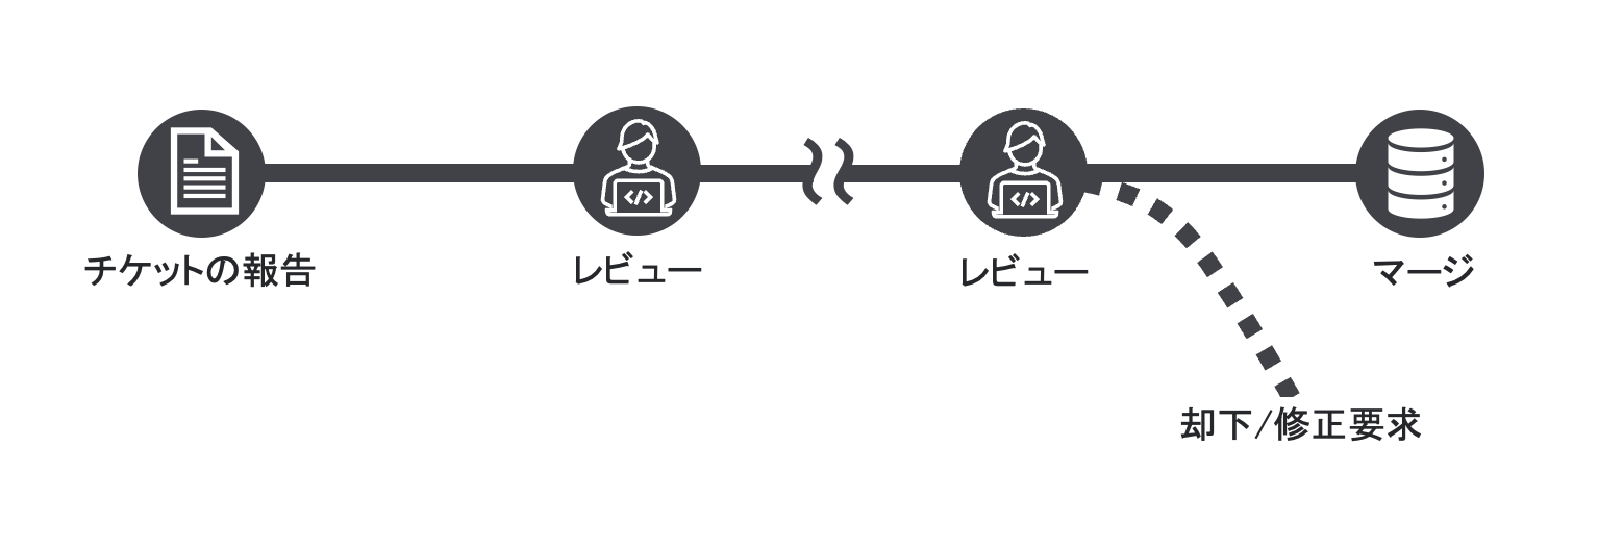
\includegraphics[width=1.0\linewidth]{Uenaka_fig/code_review_process.pdf}
}
\caption{コードレビュープロセス}
\label{fig:codereviewprocess}
\end{center}
\end{figure}
%-----------------------

\section{関連研究}
\subsection{コードレビューチケットの優先順位付け}
Veen\cite{prioritizer}らは,OSS開発を対象にコードレビューの優先順位付け手法を提案している.従来研究では,機械学習アルゴリズムを用いて,変更内容や開発者の特徴などの14種類の特徴を説明変数とし,コードレビューチケットに翌日までにレビュー結果が投稿されるか否かを予測する手法を提案している.当該研究ではリリースまでの期間などの開発状況によって日々優先順位が変動するような変更提案のチケットに対して誤った優先順位を算出することが示唆される.また,他にも様々な従来研究\cite{review_prioritize_pineapple}\cite{prioritize_azeem}\cite{prioritize_fan}において優先順位付けモデルが提案されているが,いずれの研究もリリースまでの期間に焦点を当てていない.そのため,本研究ではリリースまでの期間などの開発状況を説明変数に用いた予測モデルを構築し,開発状況を説明変数に用いていない予測モデルと予測性能を比較する.また,これらの研究\cite{prioritizer}\cite{review_prioritize_pineapple}\cite{prioritize_azeem}\cite{prioritize_fan}では各予測における評価指標の平均を予測性能として算出するため,リリースまでの期間内で予測性能がどのように変化するかについては明らかにされていない.そのため,本研究ではリリースまでの期間内におけるモデルの予測性能を1日ごとに算出することで,モデルの予測性能がどのように変化するかを明らかにする.

\subsection{開発者の貢献量がチケットのレビュー/マージ判断にもたらす影響}
Bosu\cite{review1}らは,OSS開発における開発者の貢献量がチケットのレビュー/マージ判断に影響するのか否かを明らかにするために,OSS開発に積極的に貢献する開発者と消極的な開発者がそれぞれ報告したソースコードのレビュープロセスの違いを調査した.8つのOSSプロジェクトからマージもしくは却下と判断されたチケットのコードレビューデータを調査した結果,積極的に貢献する開発者のチケットほど,レビュー開始までの時間やマージもしくは却下までの時間が短く,マージされる確率が高いことが明らかとなった.その結果から本研究では,開発者の貢献量を捉えるために,従来研究\cite{prioritizer}の説明変数であるマージ実績(開発者が過去に報告したチケットのマージ率)だけでなく,報告実績(開発者が過去に報告したチケット数),直近マージ実績(開発者が過去に報告したチケットの3ヶ月以内のマージ率),直近報告実績(開発者が過去3ヶ月以内に報告したチケット数)を説明変数に加え,優先的にレビュー/マージされるチケットを予測する.

\subsection{コードレビューにかかる時間およびマージ判断に影響を与える要因}
Kononenko\cite{release_merge}らは,コードレビューにかかる時間やマージ判断に影響を与える要因を明らかにするためにコードレビューチケットを調査し,定性的分析としてレビュアへのインタビューを行った.レビュアへのインタビュー内容を調査した結果,一部のレビュアの意見から,レビューにかかる時間は変更内容(バグ修正,リファクタリング等)によって異なることが明らかとなった.そのため,本研究では変更内容によってレビュー判断が異なると考え,従来研究\cite{bug}\cite{refactoring}において定義された正規表現をチケットのタイトルと概要に適用することで得られる特徴量を,バグ修正確信度とリファクタリングとして説明変数に加え,優先的にレビュー/マージされるチケットを予測する.
また,マージ判断はリリースまでの期間によって異なることが明らかとなった.本研究ではこの知見をキーアイデアとし,リリースまでの期間に焦点を当てた研究を実施する.

\section{本研究の動機}
ソフトウェア開発において,リリースまでの期間などの開発状況によって,優先的にレビュー/マージされるチケットの予測モデルの性能が低下することが従来研究\cite{release_merge}に基づき示唆される.
しかし,従来の優先順位付けの研究\cite{prioritizer}\cite{review_prioritize_pineapple}\cite{prioritize_azeem}\cite{prioritize_fan}は,リリースまでの期間による優先順位の変化を考慮しておらず,時期に関係なくバージョン間で共通の優先基準が存在することを前提とした研究である.
そのため,本研究では,時期ごとにバージョン間で共通の優先基準が存在し,その基準に応じてチケットが優先される場合と優先されなくなる場合があると考え,リリースまでの期間に焦点を当てた研究を行う.

本研究では,事前分析として,リリースまでの期間別にレビュー/マージされるコードレビューチケットの特徴が異なるかを分析する.また,RQ1では,従来研究\cite{prioritizer}のようなチケットおよび開発者の特徴からチケットの優先順位を予測するモデルをベースラインモデルとして構築し,リリースまでの期間内での予測性能の変化を分析する.RQ2では,時系列で変化する特徴として,従来研究\cite{integrator}\cite{release_merge}の知見から開発状況の特徴(3種類)を定義し,ベースラインモデルで用いた12種類の説明変数に追加したモデルを提案モデルとして構築し,両モデルの予測性能を比較する.

% また,データセットとして利用しているプロジェクトの検証者にアンケート調査を行うことで,分析結果を考察する.


%%%%%%%%%%%%%%%%%%%%%%
\section{事前分析:リリースまでの期間に応じた優先されるチケットの変化の有無の調査}\label{sec:pre_analysis}
%%%%%%%%%%%%%%%%%%%%%%

\section{概要}
本研究では,時期ごとにバージョン間で共通の優先基準が存在し,その基準に応じてチケットが優先される場合と優先されなくなる場合があると考える.そこで事前分析では,優先的にレビュー/マージされるコードレビューチケットの特徴量がリリースまでの期間によって異なるかを明らかにする.具体的には,図\ref{fig:labeling}に示すようにリリースまでの期間を前期,中期,後期に3分割する.そして,それぞれの期間においてチケットをレビュー開始済/非レビューやマージ済/非マージの2クラスに分類(\ref{sec:bunrui}項で後述)し,各クラスのチケット群の特徴量を計測(\ref{sec:metrics}項で後述)し,各クラスのチケット群の特徴量の有意差を算出し,各期間で比較する(\ref{sec:compare}項で後述)ことで,優先的にレビュー/マージされたチケットの特徴量の期間ごとの違いを分析する.

\section{優先されるチケットと優先されないチケットの特徴量比較}
\subsection{コードレビューチケットの分類}\label{sec:bunrui}
\textbf{(レビュー)} 本研究では各期間において,レビュアからのコメントや評価が投稿されたチケットを優先的にレビューされるチケットと捉え「レビュー開始済」に分類し,チケットの報告以降,レビュアからのコメントや評価が投稿されていないチケットを優先的にレビューされないチケットと捉え「非レビュー」に分類する.本研究では,レビューされていないチケットの中で,優先的にレビューを要すると判断されるチケットの時期に応じた特徴の違いを明らかにするため,レビューが開始されたチケットは,次の期間以降から分析対象外とする.
図\ref{fig:labeling}のチケットを例に説明すると,対象チケットは前期に報告されているものの,前期においてまだレビューされていないため,前期では「非レビュー」に分類する.また,中期においてレビューが開始されたため,中期では「レビュー開始済」に分類し,後期以降は分析対象外とする.

\textbf{(マージ)} 本研究では各期間において,GitHubリポジトリにマージされたチケットを優先的にマージされるチケットと捉え「マージ済」に分類し,チケットが報告されてからリポジトリにマージされていないチケットを優先的にマージされないチケットと捉え「非マージ」に分類する.また,レビューと同じく,「マージ済」のチケットは,次の期間以降から分析対象外とする.
図\ref{fig:labeling}のチケットを例に説明すると,対象チケットは前期に報告されているものの,前期や中期においてマージされていないため,前期や中期では「非マージ」に分類する.また,後期においてリポジトリにマージされたため,後期では「マージ済」に分類し,以降は分析対象外とする.

%-----------------------
\begin{figure}[h]
\begin{center}
\scalebox{1.2}{
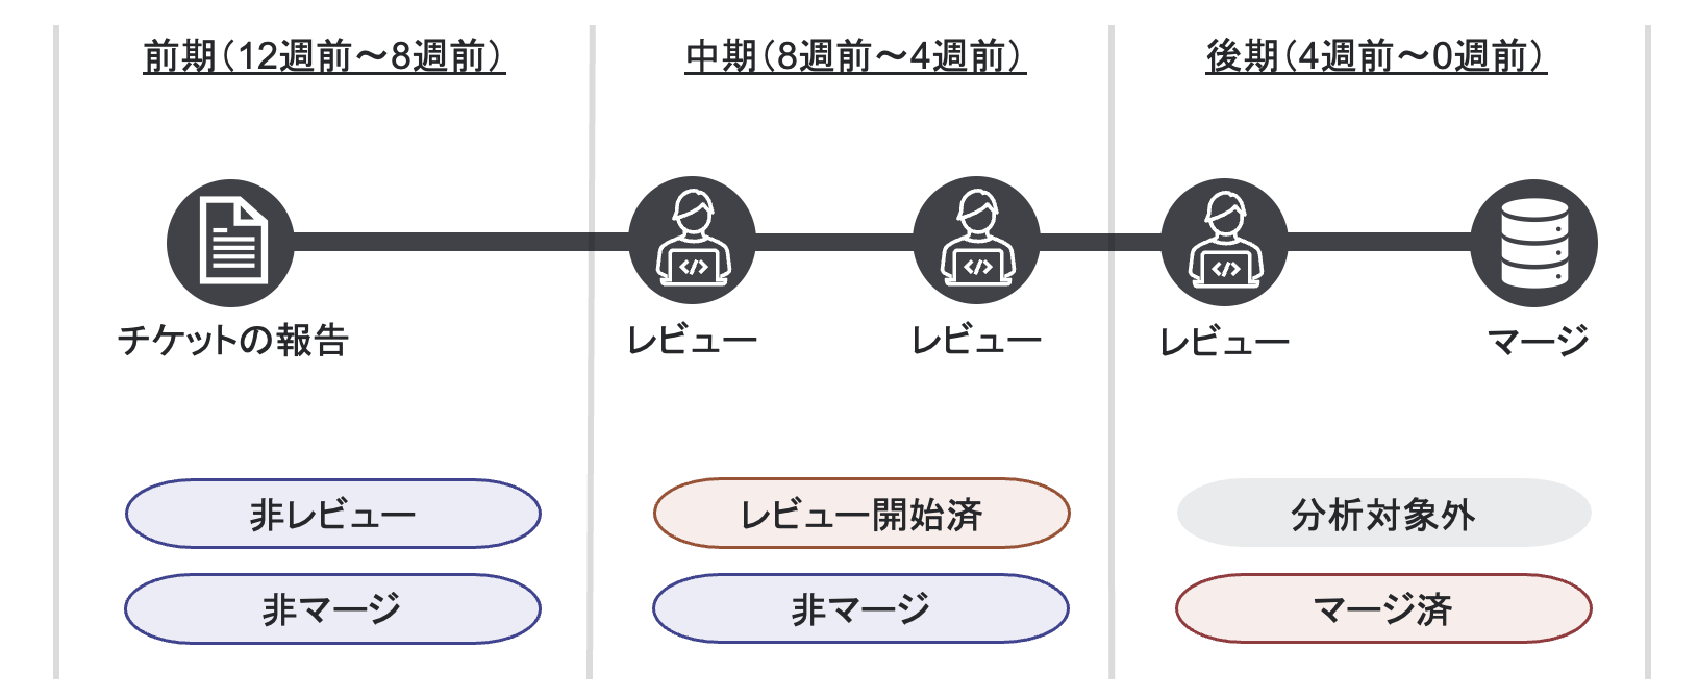
\includegraphics[width=0.8\linewidth]{Uenaka_fig/classification_method.pdf}
}
\caption{チケットの分類例}
\label{fig:labeling}
\end{center}
\end{figure}
%-----------------------


\subsection{コードレビューチケットの特徴量の計測}\label{sec:metrics}
事前分析では,\ref{sec:bunrui}項において2クラスに分類したチケットから特徴量を計測する.本分析では,時系列によって値が変化する特徴量を用いているため,同一の変更提案でもリリースまでの期間ごとに特徴量を再計測する.そのため特徴量の計測タイミングは2種類あり,期間内に報告されたチケットは報告時点の特徴量を計測し,既に報告されていたチケットは各期間の開始時点の特徴量を計測する.図\ref{fig:labeling}のチケットを例に説明すると,対象チケットは前期に報告されているため,前期では報告時点の特徴量を計測し,中期や後期では各期間の開始時点の特徴量を計測する.
具体的に事前分析で用いる特徴量について説明する.事前分析では,表\ref{table:metrics}に示す12種類の特徴量を\ref{sec:bunrui}項において2クラスに分類したチケットから計測する.12種類の特徴量は,従来研究\cite{prioritizer}において用いられていた特徴量や,従来研究\cite{release_merge}\cite{review1}の知見から有用と示唆される特徴量である.ただし,従来研究\cite{prioritizer}において用いられていた特徴量のうち,コミット数のようなGitHub特有の特徴量は計測対象外とする.
従来研究\cite{release_merge}\cite{review1}の知見から有用と示唆される特徴量のうち,バグ修正確信度は従来研究\cite{bug}において利用されていた正規表現をチケットのタイトルと概要に適用することで,チケットがバグである確度を3クラスに分類した特徴量である.
%なお,本研究では報告実績等の時系列によって値が変化する特徴量を用いているため,同一の変更提案でもリリースまでの期間ごとに再計測する.

%-----------------------
\begin{table}[h]
  \caption{事前分析に用いる12種類の特徴量}
  \label{table:metrics}
  \centering
  \vspace{0.5zh}
    \scalebox{1.02}{
  \begin{tabular}{l|l|l}
    \hline \hline
    \multicolumn{1}{c|}{特徴量}  & \multicolumn{1}{c|}{説明}  & \multicolumn{1}{c}{従来研究}  \\
    \hline
    報告実績  & 開発者が過去に報告したチケット数  & \cite{review1} \\
    直近報告実績  & 開発者が過去3ヶ月以内に報告したチケット数  & \cite{review1} \\
    マージ実績  & 開発者が過去に報告したチケットのマージ率  & \cite{review1},\cite{prioritizer} \\
    直近マージ実績  & 開発者が過去3ヶ月以内に報告したチケットのマージ率  & \cite{review1} \\
    追加行数  &  チケットで追加されている変更行数  & \cite{prioritizer},\cite{diff} \\
    削除行数  & チケットで削除されている変更行数  & \cite{prioritizer},\cite{diff}  \\
    ファイル数  & チケットで変更されているファイル数  & \cite{prioritizer} \\
    リビジョン数  & チケットの分析時点のリビジョン数  & \cite{prioritizer} \\
    経過時間  & チケットが報告されてからの経過時間  & \cite{prioritizer} \\
    テストコード含有  & 変更ファイルにテストが含まれているか  & \cite{prioritizer} \\
    バグ修正確信度  &  バグ修正の変更提案である確度  & \cite{bug},\cite{release_merge} \\
    リファクタリング  & リファクタリングの変更提案か否か  & \cite{refactoring},\cite{release_merge} \\
    \hline
  \end{tabular}
  }
\end{table}
%-----------------------

\subsection{コードレビューチケットの特徴量の比較}\label{sec:compare}
前期,中期,後期の3期間において優先的にレビュー/マージされるコードレビューチケットの特徴量を分析する.具体的には,各期間におけるレビュー開始済チケットと非レビューチケット間や,マージ済チケットと非マージチケット間の各特徴量の統計的有意差を算出する.統計検定手法として,比例尺度の特徴量に対してはマンホイットニーのU検定,名義尺度の特徴量に対してはカイ2乗検定を用いてP値を算出することで,統計的有意差の有無を明らかにする.有意差がある場合,当該期間における2クラス(レビュー開始済チケットと非レビューチケット,もしくはマージ済チケットと非マージチケット)間の特徴量に違いがあることを示す.

また,リリースまでの期間による各特徴量の有意差の違いを分析することで,リリースまでの期間によって優先的にレビュー/マージされるチケットの特徴量が異なるかを明らかにする.具体的には,前期では統計的有意差の無い特徴量Aに,後期では統計的有意差がある場合,特徴量Aは前期ではチケットのレビュー/マージ判断に影響しない一方で,後期ではチケットのレビュー/マージ判断に影響することが示唆される.つまり,リリースまでの期間によってレビュー/マージ判断における特徴量Aの重要度が変化すると解釈する.


\section{データセット}\label{sec:dataset}
本研究では,OpenStackプロジェクトのうち,コアコンポーネント6プロジェクト(Nova,Neutron,Cinder,Keystone,Swift,Glance)を分析対象とし,各プロジェクトの変更提案の中で,立ち上げ時から2022年9月までにマージもしくは却下されたコードレビューチケットを収集した.変更提案のチケットの特徴量を計測するために,OpenStackがコードレビュー管理システムとして使用するGerrit\footnote{Gerrit: \url{https://review.opendev.org}}から,コードレビュー履歴を収集した.また各バージョンのリリース日を特定するために,Gitから各バージョンのリリース履歴を収集した.各チケットがマージされたリリースを特定するために,Gitから各プロジェクトのコミット履歴を収集し,コミットの親子関係を追跡した.

本研究では,各プロジェクトで5つのバージョンリリースまでにレビュー/マージされたコードレビューチケットの変更提案を対象とする.分析対象プロジェクトのリリース間隔が約3ヶ月であるため,特にリリース直前の3ヶ月にマージされたチケット数上位5バージョンを分析対象とすることで,「マージ済」に分類されるチケットの多いバージョンを対象とした分析を行う.表\ref{table:release}は分析対象とする各プロジェクトのバージョンを示す.また,長期間に渡り放置される変更提案は,短期的な優先順位の決定には関与しないため,リリース直前の6ヶ月以内に提出されたチケットを分析対象とする.

%------------------------
\begin{table*}[h]
\centering
  \caption{プロジェクトごとの対象リリースバージョン}
  \vspace{0.5zh}
  \label{table:release}
  \scalebox{0.80}{
  \begin{tabular}{l|r|l}  \hline \hline
    プロジェクト & チケット数 & \multicolumn{1}{c}{バージョン(リリース3ヶ月以内にマージされたチケット数 )}\\ \hline 
    Nova & 39,870 & 13.0.0.0b3(529),14.0.0.0b1(475),16.0.0.0b2(451),17.0.0.0b1(410),20.0.0.0rc1(392)\\ 
    Neutron & 24,467 & 7.0.0.0b1(326),8.0.0.0b1(400),9.0.0.0b1(296),11.0.0.0b1(286),16.0.0.0b1(186)\\ 
    Cinder & 17,155 & 8.0.0.0b1(249),8.0.0.0rc1(249),9.0.0.0b2(249),11.0.0.0b2(249),12.0.0.0b2(235)\\ 
    Keystone & 10,764 & 8.0.0a0(182),9.0.0.0b3(211),10.0.0.0b2(220),11.0.0.0b1(167),15.0.0.0rc1(165)\\ 
    Swift & 8,737 & 1.9.2(180),2.4.0(154),2.7.0(117),2.17.0(105),2.27.0(101)\\ 
    Glance & 6,248 & 11.0.0a0(70),12.0.0.0b1(83),12.0.0.0b3(72),13.0.0.0b1(64),17.0.0.0b1(73)\\ \hline
  \end{tabular}
  }
\end{table*}
%------------------------

\section{リリースまでの期間に応じた優先されるチケットの変化}
事前分析では,リリースまでの期間(前期,中期,後期)に応じて,レビュー開始済/非レビューのチケットやマージ済/非マージのチケットの特徴量の間の統計的有意差を算出することで,チケットの特徴量を比較する.結果の表では,P値が0.01未満は***,0.01〜0.05は**,0.05〜0.1は*で表記する.

%--------------------
\begin{table*}[h]
\caption{レビュー開始済チケットと非レビューチケットの特徴量の検定結果}
\label{table:review_notreview_prepare}
\centering
\vspace{0.5zh}
\scalebox{0.72}{
\begin{tabular}{l|ccc|ccc|ccc|ccc|ccc|ccc}
    \hline \hline
    \multirow{2}{*}{特徴量} & \multicolumn{3}{c|}{Nova} & \multicolumn{3}{c|}{Neutron} & \multicolumn{3}{c|}{Cinder} & \multicolumn{3}{c|}{Keystone} & \multicolumn{3}{c|}{Swift} & \multicolumn{3}{c}{Glance} \\ \cline{2-19}
    & 前 & 中 & 後 & 前 & 中 & 後 & 前 & 中 & 後 & 前 & 中 & 後 & 前 & 中 & 後 & 前 & 中 & 後 \\ \hline
    マージ実績 & *** & *** & *** & *** & *** & *** &  & * & *** &  & ** & *** &  &  &  & *** & *** & *** \\
    直近マージ実績 & *** & *** & *** & *** & *** & *** &  & * & *** & * &  & *** &  & *** & *** & *** & ** & *** \\
    報告実績 &  &  &  &  &   & *** & ** & *** &  & *** & *** &   &  & * & *** & ** &  &  \\
    直近報告実績 &  & ** & *** & ** &   & *** & * & ** &  & *** & *** &   & * &  & ** &  &  &  \\
    追加行数 & *** & *** & *** & *** & *** & *** & * & *** & *** & *** & *** & *** & *** & *** & *** & *** & *** & *** \\
    削除行数 & * &  &  & *** & * &  &  &  & ** &  &  &  & ** & *** &  &  &   &  \\
    ファイル数 & *** & *** & *** & *** & *** & *** &  & ** & * & *** & * & *** & *** & *** & *** & *** & *** & *** \\
    リビジョン数 & *** & *** & *** & *** & *** & *** & *** & *** & *** & *** & *** & *** & *** & *** & *** & *** & *** & *** \\
    経過時間 & *** & *** & *** & *** & *** & *** & ** & * & *** & *** & *** & *** & *** & *** & *** & *** & *** & *** \\
    テストコード含有 & *** & *** &  &  &  & ** &  &  & * & *** &   & * &  &  &  &  & * &  \\
    バグ修正確信度 & *** & *** & *** & *** & *** & *** & *** & *** & *** & ** &   & * &  &  &  & *** & ** & *** \\
    リファクタリング &  &  &  &  & * &  &  & ** & ** & ** &   &  &  &   &  &    &   &  \\ \hline
\end{tabular}}


\vspace{2mm}
\caption{マージ済チケットと非マージチケットの特徴量の検定結果}
\label{table:merge_notmerge_prepare}
\centering
\vspace{0.5zh}
\scalebox{0.72}{
\begin{tabular}{l|ccc|ccc|ccc|ccc|ccc|ccc}
    \hline \hline
    \multirow{2}{*}{特徴量} & \multicolumn{3}{c|}{Nova} & \multicolumn{3}{c|}{Neutron} & \multicolumn{3}{c|}{Cinder} & \multicolumn{3}{c|}{Keystone} & \multicolumn{3}{c|}{Swift} & \multicolumn{3}{c}{Glance} \\ \cline{2-19}
    & 前 & 中 & 後 & 前 & 中 & 後 & 前 & 中 & 後 & 前 & 中 & 後 & 前 & 中 & 後 & 前 & 中 & 後 \\ \hline
    マージ実績 & *** & *** & *** & *** & *** & *** & *** & *** & *** & *** & *** & *** & *** & *** & *** & *** & *** & *** \\
    直近マージ実績 & * & *** & *** & *** & *** & *** & * & * & *** & *** & *** & *** & *** & ** & *** & * & ** &  \\
    報告実績 & *** & *** & *** & *** & *** & *** & *** & *** & *** & *** & *** & *** & * &  &  & *** & * &  \\
    直近報告実績 &  &  & *** &  &  & *** & ** &  & * & *** & *** & *** & *** & *** & *** &  &  &  \\
    追加行数 & *** & *** & *** & *** & *** & *** & *** & *** & *** & * & *** & *** & *** & *** & *** & * & *** & *** \\
    削除行数 &   &  &  & ** &  &   &  & ** &  &   &   &   &   &    & * &  &  & ** \\
    ファイル数 & *** &  &  & ** & * & ** &  &  &  &  &  &  & * & * &  & ** &  &  \\
    リビジョン数 &  &  & *** & * &  & *** &  &  &  &  &  &  &  & ** & * & *** &  &  \\
    経過時間 &  & *** & *** & *** & *** &  &  & ** & *** &  & ** & *** &  & *** &  & *** & * & ** \\
    テストコード含有 & *** & *** & *** & *** & *** & *** &  & *** &  & *** & *** & ** &  & * & ** & *** & ** &    \\
    バグ修正確信度 & *** & *** & *** & *** & *** & *** & *** & *** &  &  & *** & * &  & ** &  & * & ***  & *** \\
    リファクタリング & *** &   & ** &  &  &  & ** &   &   &   &   &  & * &   & ** & ** & * & * \\ \hline
\end{tabular}}
\end{table*}
%--------------------

\textbf{(レビュー)} 表\ref{table:review_notreview_prepare}は,各プロジェクトの前期,中期,後期におけるレビュー開始済チケットと非レビューチケット間の特徴量の検定結果を示す.表\ref{table:review_notreview_prepare}の結果から,多くのプロジェクトにおいて追加行数,リビジョン数,経過時間の特徴量はいずれの期間でもレビュー開始済/非レビューのチケット間で統計的に有意な差があることを確認した.したがって,追加行数,リビジョン数,経過時間はどの時期でもチケットのレビュー判断に影響することが示唆される.次に,マージ実績はCinderプロジェクトやKeystoneプロジェクトにおいて,前期では統計的有意差を確認できなかったが,中期や後期それぞれでは統計的有意差を確認できた.したがって,CinderプロジェクトやKeystoneプロジェクトにおいて,マージ実績は前期ではチケットのレビュー判断に影響しない一方で,中期や後期ではチケットのレビュー判断に影響する,つまりリリースまでの期間によってレビュー判断におけるマージ実績の重要度が変化することが示唆される.マージ実績の他にも,報告実績,テストコード含有などの特徴量は,複数プロジェクトにおいて統計的有意差の有無が変化したため,レビュー判断において重要度が変化することが示唆される.
図\ref{fig:review_notreview}は,統計的有意差の有無が変化した特徴量の一例として,Cinderプロジェクトのレビュー開始済チケットと非レビューチケットのマージ実績の分布を示す.横軸はリリースまでの期間,縦軸はマージ実績を表し,各期間における箱髭図は左がレビュー開始済チケット,右が非レビューチケットにおけるマージ実績を表している.図\ref{fig:review_notreview}の結果から,後期におけるレビュー開始済チケットと非レビューチケットをそれぞれ報告した開発者のマージ実績(中央値の差)は,前期や中期に比べて大きく,後期にはマージ実績の高い開発者が報告したチケットが優先的にレビューされていることが示唆される.したがって,リリースまでの期間に応じてレビューされるチケットの特徴には違いがあることが示唆された.


%-----------------------
\begin{figure}[h]
\begin{center}
\scalebox{0.95}{
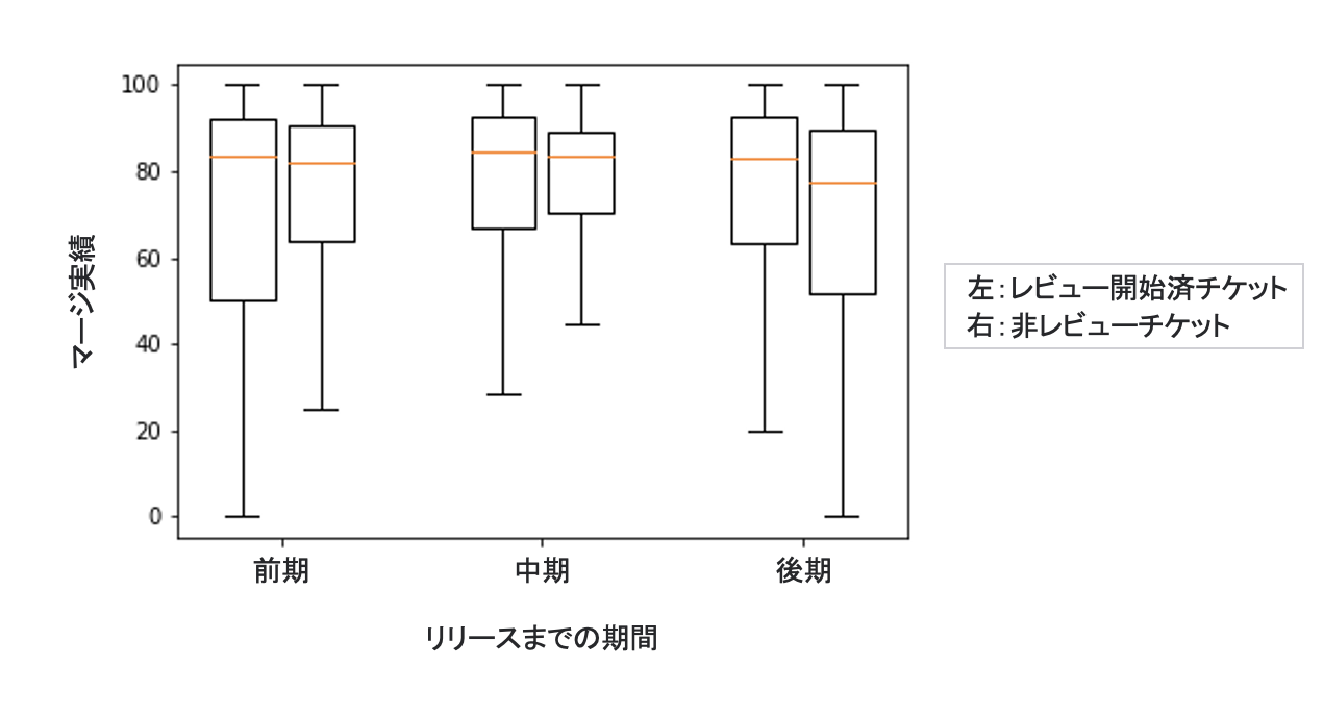
\includegraphics[width=0.8\linewidth]{Uenaka_fig/review_notreview.pdf}
}
\caption{Cinderプロジェクトにおけるレビュー開始済/非レビューのチケットのマージ実績の分布}
\label{fig:review_notreview}
\end{center}
\end{figure}
%-----------------------

\textbf{(マージ)} 表\ref{table:merge_notmerge_prepare}は各プロジェクトの前期,中期,後期におけるマージ済チケットと非マージチケット間の特徴量の検定結果を示す.表\ref{table:merge_notmerge_prepare}の結果から,マージ実績,追加行数の特徴量は全てのプロジェクトの全期間において,マージ済/非マージのチケット間で統計的に有意な差があった.この結果から,マージ実績,追加行数はどの時期でもチケットのマージ判断に影響することが示唆される.
次に,経過時間はNova,Cinder,Keystoneプロジェクトにおいて,前期では統計的有意差を確認できなかったが,中期や後期それぞれでは統計的有意差を確認できた.したがって,Nova,Cinder,Keystoneプロジェクトにおいて,経過時間は前期ではチケットのマージ判断に影響しない一方で,中期や後期ではチケットのマージ判断に影響する,つまりリリースまでの期間によってマージ判断における経過時間の重要度が変化することが示唆される.また,Neutron,Swift,Glanceプロジェクトにおいても前述の3プロジェクトとは異なったリリースまでの期間において統計的有意差の有無が変化したため,これらの3プロジェクトでもリリースまでの期間によってマージ判断における経過時間の重要度が変化することが示唆される.経過時間の他にも,直近マージ実績,バグ修正確信度などの特徴量は,複数プロジェクトにおいて統計的有意差の有無が変化したため,マージ判断において重要度が変化することが示唆される.
図\ref{fig:merge_age}は,統計的有意差の有無が変化した特徴量の一例として,Keystoneプロジェクトのマージ済チケットと非マージチケットの経過時間の分布を示す.横軸はリリースまでの期間,縦軸は経過時間を表し,各期間における箱髭図は左がマージ済チケット,右が非マージチケットにおける経過時間を表している.図\ref{fig:merge_age}の結果から,後期におけるマージ済チケットと非マージチケットの経過時間(中央値の差)は,前期や中期に比べて大きく,後期には経過時間の短いチケットが優先的にマージされていることが示唆される.したがって,リリースまでの期間に応じてマージされるチケットの特徴には違いがあることが示唆された.

%-----------------------
\begin{figure}[h]
\begin{center}
\scalebox{0.85}{
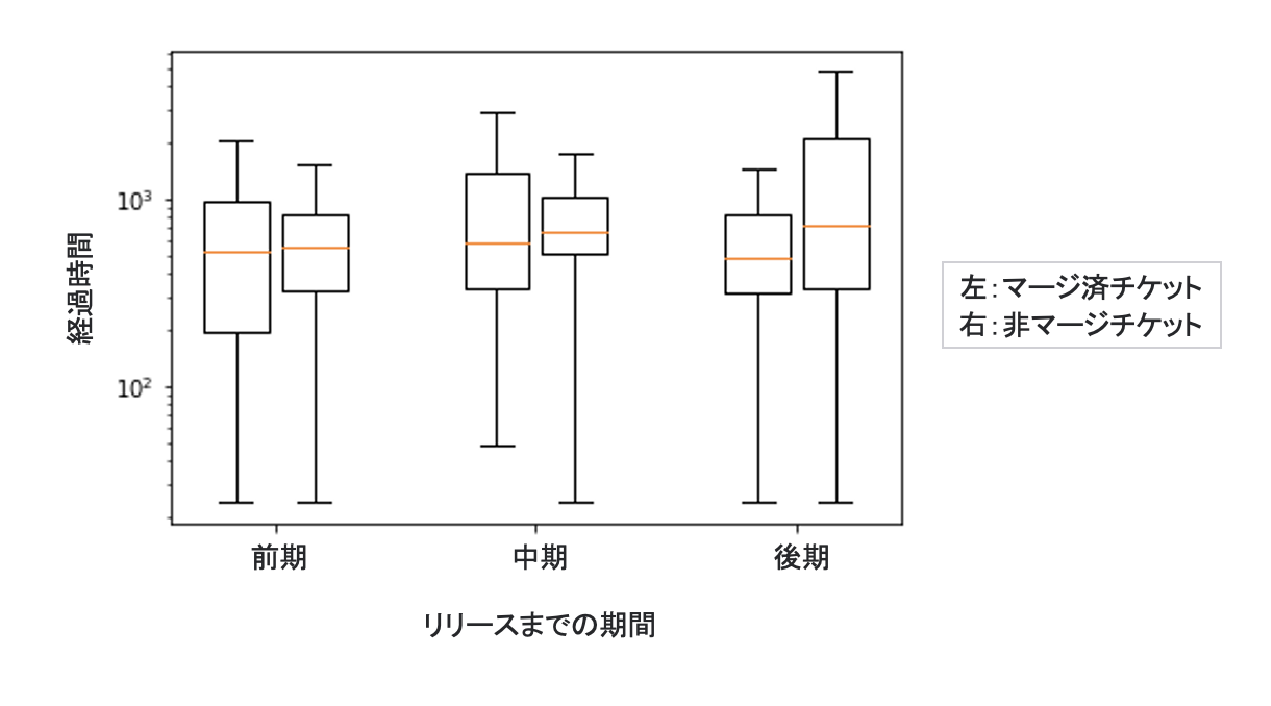
\includegraphics[width=0.8\linewidth]{Uenaka_fig/merge_age.pdf}
}
\caption{Keystoneプロジェクトにおけるマージ済/非マージのチケットの経過時間の分布}
\label{fig:merge_age}
\end{center}
\end{figure}
%-----------------------

\fbox{\parbox{0.95\linewidth}{\textbf{(結果のまとめ)} 複数プロジェクトにおいて,リリースまでの期間に応じてレビュー/マージされるチケットの特徴には違いがある.また,各リリースまでの期間において,プロジェクトによって優先的にレビュー/マージされるチケットの特徴は異なる.}}


%%%%%%%%%%%%%%%%%%%%%%%%%%%%%%%%%
\section{開発状況に基づく優先的にレビュー/マージされるコードレビューチケットの特定手法と評価方法}\label{sec:analysis_method}
%%%%%%%%%%%%%%%%%%%%%%%%%%%%%%%%%

RQ1では,従来手法と同様にチケットおよび開発者の特徴を説明変数とするモデル(ベースラインモデル)を構築し,リリースまでの期間内においてベースラインモデルの予測性能がどの程度変化するかを明らかにする.また,RQ2では,開発状況の特徴を追加で説明変数とするモデル(提案モデル)を構築し,開発状況に関する説明変数を用いることで,リリースまでの期間内で予測性能がどの程度変化するかを明らかにする.
具体的には,ウィンドウサイズを2週間とするスライディングウィンドウを定義し,1日ずつずらしながら予測モデルの学習およびテストを行うことでモデルの予測性能の変化を時系列的に分析し,予測性能を比較することでRQを検証する.
\ref{sec:koutiku}節で予測モデルの構築方法,\ref{sec:kenshou}節で予測モデルの検証方法,\ref{sec:hyoka}節で予測モデルの評価方法を述べる.


\section{予測モデルの構築}\label{sec:koutiku}

\subsection{説明変数の計測}\label{sec:setumeihensuu}
本分析では,\ref{sec:metrics}節で計測したチケットおよび開発者の特徴量のみを説明変数とするモデル(ベースラインモデル)と,時系列で変化する特徴を追加で説明変数とするモデル(提案モデル)の2種類のモデルを構築する.本分析では,従来研究\cite{integrator}\cite{release_merge}の知見から,リリースまでの残り時間,レビュアの抱えているタスク,レビュアが対応できるレビュー上限の3種類を時系列で変化する特徴として定義する.時系列で変化する特徴を表\ref{table:metrics_kaihatujoukyou}に示す3種類の開発状況の特徴に置き換えることで,提案モデルの説明変数として計測する.
なお,本分析ではウィンドウサイズを2週間とするスライディングウィンドウを定義し,1日ずつずらしながら予測モデルの学習を行うため,各ウィンドウでチケットから説明変数を計測する.このとき,ウィンドウの期間内に報告されたチケットは報告時点の説明変数を計測し,ウィンドウの期間前に報告されていたチケットはウィンドウの開始時点の説明変数を計測する.また,本分析では報告実績等の時系列によって値が変化する特徴量を説明変数に用いているため,同一の変更提案でも各ウィンドウで再度計測する.

本研究では,上記のような説明変数を学習させることで,ベースラインモデルとしてリリース期間全体を通してレビュー/マージされるチケットと類似した特徴を持つチケットを正しく判別できるモデルを構築する.また,提案モデルとしてリリース期間全体を通してレビュー/マージされるチケットと類似した特徴を持つチケットだけでなく,開発状況によってレビュー/マージされるか否かが変化するようなチケットを正しく判別できるモデルを構築する.

%-----------------------
\begin{table}[h]
  \caption{説明変数として計測する開発状況}
  \label{table:metrics_kaihatujoukyou}
  \centering
  \vspace{0.5zh}
    \scalebox{1.02}{
  \begin{tabular}{l|l|l}
    \hline \hline
    \multicolumn{1}{c|}{説明変数}  & \multicolumn{1}{c|}{説明}  & \multicolumn{1}{c}{従来研究}  \\
    \hline
    リリースまでの残り日数  & ウィンドウ内の最新日からリリース日までの日数  & \cite{release_merge} \\
    予測対象チケット数  & ウィンドウ内の予測対象であるチケット数  & \cite{integrator} \\
    レビュアのレビュー行数  & ウィンドウ内でレビューされた総行数  & \cite{integrator} \\
    \hline
  \end{tabular}
  }
\end{table}
%-----------------------

\subsection{目的変数の計測}
\textbf{(レビュー予測モデル)}本分析では,レビュー予測モデルとしてレビューが開始されるか否かを目的変数としたモデルを構築する.具体的には,報告されてから初めてレビュアからのコメントや評価が投稿された日をレビューが開始された日と定義し,ウィンドウ内の2週間においてレビューが開始されたチケットを正例クラス,レビューが開始されないチケットを負例クラスとして計測する.また,本分析ではレビューが開始されていないチケットの中で,優先的にレビューを要すると判断されるチケットの予測性能を明らかにするために,ウィンドウ内の2週間より前にレビューが開始されたチケットに関しては,既に優先されたチケットとみなし分類対象外とする.

\textbf{(マージ予測モデル)}本分析では,マージ予測モデルとして直近のリリースにマージされるか否かを目的変数としたモデルを構築する.具体的には,報告されてから初めてGitHubリポジトリにマージされた日をマージされた日と定義し,ウィンドウ内の2週間においてマージされたチケットを正例クラス,マージされないチケットを負例クラスとして計測する.また,本分析ではマージされていないチケットの中で,優先的にマージすべきであると判断されるチケットの予測性能を明らかにするために,ウィンドウ内の2週間より前にマージされたことのあるチケットに関しては,既に優先されたチケットとみなし分類対象外とする.また,OpenStackがコードレビュー管理システムとして使用しているGerritでは,一度もレビューされていないチケットはマージできない仕様となっている.そのため,マージされたことのないチケットの中でも,レビューが開始されていないチケットに関しては,マージされないことが確定しているチケットとみなし分類対象外とする.

\subsection{モデルの構築方法}
本分析では,レビューが開始されるか否か,直近のリリースにマージされるか否かをそれぞれ目的変数とする予測モデル(レビュー予測モデル,マージ予測モデル)を構築する.モデルの構築にあたっては,テストコード含有やリファクタリングか否かといった名義尺度の説明変数をダミー変数に変換した上で,\ref{sec:setumeihensuu}項で計測した説明変数をベースラインモデルでは12次元,提案モデルでは15次元のベクトルに変換して入力する.
レビュー予測モデルおよびマージ予測モデルの構築には,それぞれ機械学習アルゴリズムであるRandom Forestsモデル\cite{randomforest}を用いる.しかし,本分析では目的変数が不均衡なデータを扱うため,不均衡データに対応したBalanced Random Forestモデル\footnote{imblearn.ensemble.BalancedRandomForestClassifier: \url{https://imbalanced-learn.org/stable/references/generated/imblearn.ensemble.BalancedRandomForestClassifier.html}}を用いる.

\section{予測モデルの検証}\label{sec:kenshou}
本分析では,スライディングウィンドウを用いて1日ごとにモデルの予測性能を検証する.図\ref{fig:predict_schematic}は,予測モデルの検証方法の概略図を示す.本分析では,リリースの12週間前から1日ごとに2クラス分類モデル(提案モデル,ベースラインモデル)のテストを行う.具体的には,ウィンドウサイズを2週間とするスライディングウィンドウを定義し,ウィンドウ内のチケットを用いてテストを行うことで,各テストにおいて正例クラスのチケット(レビューが開始される/マージされるチケット)を一定数確保する.定義したウィンドウを1日ずつずらしながらテストを行うことで,リリースまでの期間内においてモデルの予測性能が変化するかを明らかにする.また,提案モデルとベースラインモデルの予測性能を比較し,開発状況に関する説明変数を用いることで,モデルの予測性能が変化するかを明らかにする.本研究では説明の都合上,以降は各ウィンドウをウィンドウN(最もリリースから遠いウィンドウはN=71,1日ずらすごとにN$-$1し,最もリリースに近いウィンドウはN=1)と定義する.

分析対象とするデータセットには\ref{sec:dataset}節で利用したOpenStackの6つのコアコンポーネントプロジェクトの5バージョンずつを用いる.具体的には,5バージョンのうち最も直近にリリースされたバージョンをテストデータとし,残りの4バージョンを学習データとして予測モデルを検証する.

%-----------------------
\begin{figure}[t]
\begin{center}
\scalebox{1.25}{
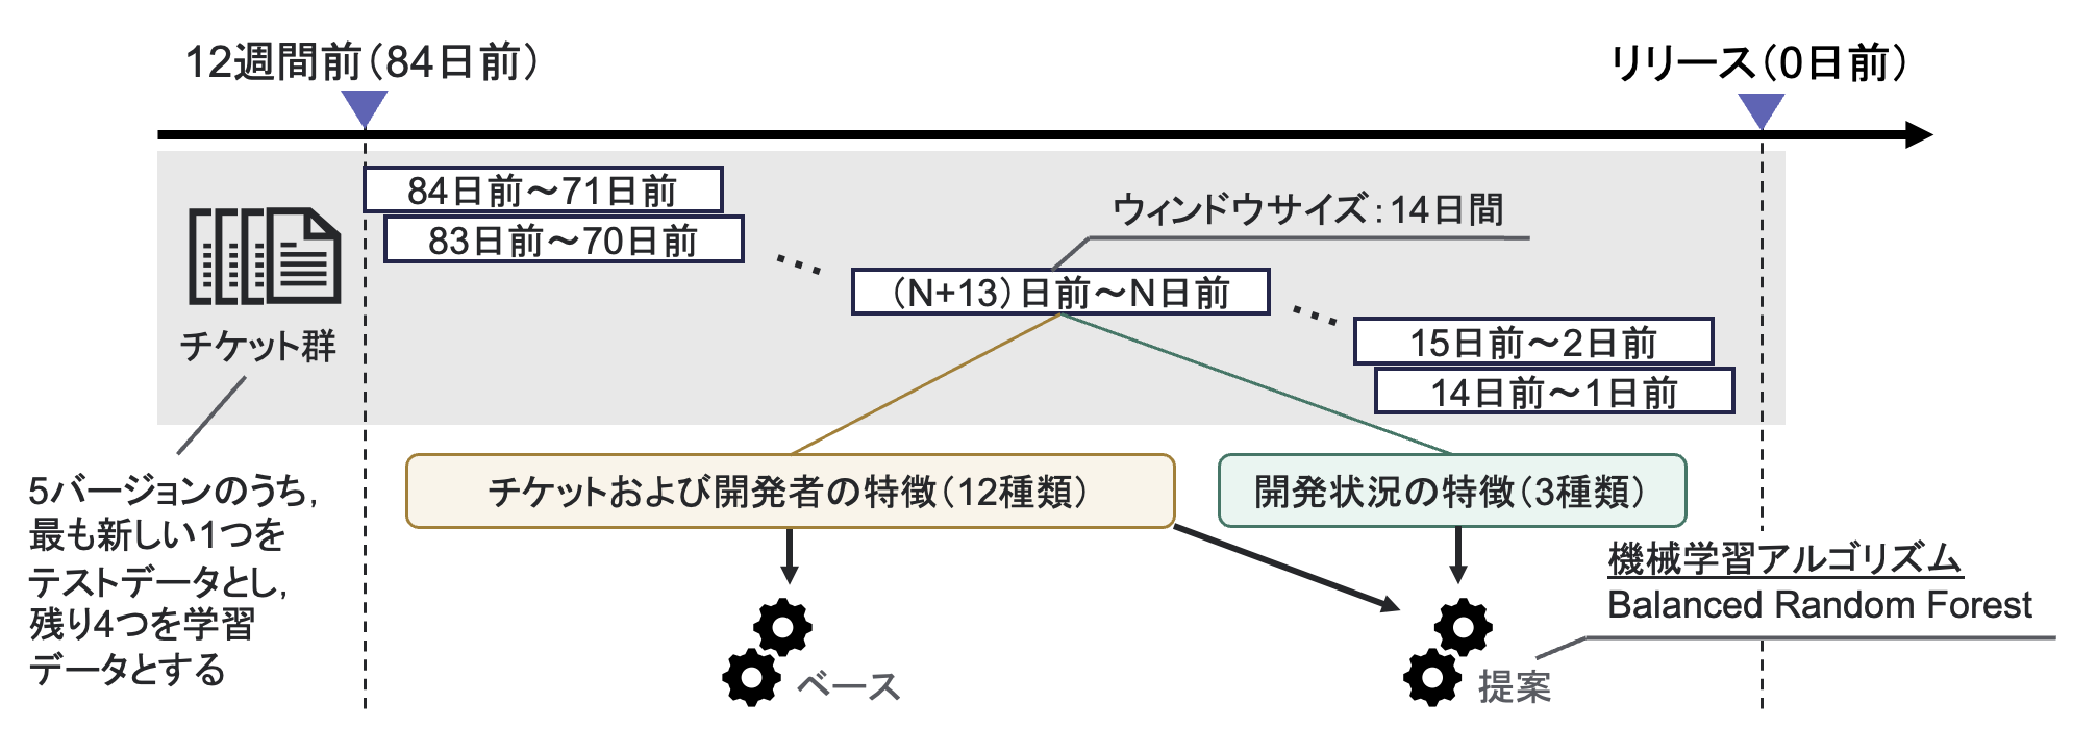
\includegraphics[width=0.8\linewidth]{Uenaka_fig/predict_schematic.pdf}
}
\caption{予測モデルの検証方法の概略図}
\label{fig:predict_schematic}
\end{center}
\end{figure}
%-----------------------


\section{予測モデルの評価}\label{sec:hyoka}
本分析では,提案モデルおよびベースラインモデルの予測性能の評価指標として適合率,再現率,F値を用いる.また,本研究では,時期ごとにバージョン間で共通の優先基準が存在し,その基準に応じてチケットが優先される場合と優先されなくなる場合があると考える.したがって,本分析では,適合率,再現率,F値に加え,優先されないチケットの予測性能の評価のために特異度を用いることで,両モデルの予測性能を比較する.
評価指標の算出にあたって,両モデルの予測結果を以下の4つに分類する.

%-----------------------
\begin{itemize}
  \item \textbf{True Positive(TP):}レビューが開始された/マージされたチケットに対して,レビューが開始された/マージされたと正しく予測するケース
  \item \textbf{False Positive(FP):}レビューが開始されない/マージされないチケットに対して,レビューが開始された/マージされたと誤って予測するケース
  \item \textbf{True Negative(TN):}レビューが開始されない/マージされないチケットに対して,レビューが開始されない/マージされないと正しく予測するケース
  \item \textbf{False Negative(FN):}レビューが開始された/マージされたチケットに対して,レビューが開始されない/マージされないと誤って予測するケース
\end{itemize}
%-----------------------

以上の4つに分類した両モデルの予測結果に基づいて,以下のように適合率,再現率,特異度,F値を算出する.

適合率は,式(\ref{precision})に示すように,レビューが開始された/マージされたとモデルが予測したチケットの中で,レビューが開始された/マージされたチケットの割合を表す.適合率は0から1の間で算出され,値が大きいほどモデルの予測の正確性が高いことを表す.

% %-----------------------
% \begin{equation}
%  適合率 = \frac{TP}{TP+FP} \label{precision}
% \end{equation}
% %-----------------------
% \vskip\baselineskip

再現率は,式(\ref{recall})に示すように,レビューが開始された/マージされたチケットの中で,レビューが開始された/マージされたとモデルが予測したチケットの割合を表す.再現率は0から1の間で算出され,値が大きいほどモデルの正例の網羅率が高いことを表す.

% %-----------------------
% \begin{equation}
%  再現率 = \frac{TP}{TP+FN} \label{recall}
% \end{equation}
% %-----------------------
% \vskip\baselineskip

特異度は,式(\ref{specificity})に示すように,レビューが開始されない/マージされないチケットの中で,レビューが開始されない/マージされないとモデルが予測したチケットの割合を表す.特異度は0から1の間で算出され,値が大きいほどモデルの負例の網羅率が高いことを表す.

%-----------------------
\begin{equation}
 \text{特異度} = \frac{TN}{TN+FP} \label{specificity}
\end{equation}
%-----------------------
\vskip\baselineskip

F値は,式(\ref{F1})に示すように,適合率と再現率の調和平均を表す.F値は0から1の間で算出され,値が大きいほどモデルの予測性能が高いことを表す.

% %-----------------------
% \begin{equation}
%  F値 = 2 * \frac{適合率*再現率}{適合率+再現率} \label{F1}
% \end{equation}
% %-----------------------
\vskip\baselineskip




%%%%%%%%%%%%%%%%%%%%%%%%%%%%%%%%%
\section{RQ1:\rqone}\label{sec:rq1}
%%%%%%%%%%%%%%%%%%%%%%%%%%%%%%%%%
RQ1では,従来手法と同様に,チケットおよび開発者の特徴を説明変数とするモデル(ベースラインモデル)を構築する.ベースラインモデルの予測性能を\ref{sec:kenshou}節の検証方法および\ref{sec:hyoka}節の評価方法に基づいて1日ごとに算出することで,従来手法の予測性能はリリースまでの期間内でどの程度変化するかを明らかにする.
\ref{sec:rq1_result}節で予測結果を述べ,\ref{sec:rq1_kousatu1}節および\ref{sec:rq1_kousatu2}節で結果について考察し,\ref{sec:rq1_matome}節でまとめる.

\section{予測結果}\label{sec:rq1_result}
\subsection{レビュー予測モデル}\label{sec:rq1_review}
図\ref{fig:review_base}は各プロジェクトにおけるベースラインモデルの予測性能を示す.図は横軸が各ウィンドウ,縦軸が予測性能を表しており,青の折れ線が適合率,緑の折れ線が再現率,紫の折れ線が特異度,赤の折れ線がF値を表す.図は左から右に向かってリリースに近いウィンドウ(最も左はウィンドウ71,最も右はウィンドウ1)での予測結果を表す.また,表\ref{table:review_hyoka_max}は各プロジェクトのレビュー予測モデルにおける予測性能の範囲(最小値〜最大値)および変動幅を示す.

表\ref{table:review_hyoka_max}における予測性能の変動幅から,リリースまでの期間内において,従来手法の予測の正確性(適合率)は0.31〜0.53,正例の網羅率(再現率)は0.19〜0.53,負例の網羅率(特異度)は0.29〜0.52,予測性能(F値)は0.16〜0.49の変動幅で変化するという結果が得られた.また,4プロジェクト (Neutron, Keystone, Swift, Glance) では全ての評価指標が0.30以上の変動幅であった一方,2プロジェクト (Nova, Cinder) では一部の評価指標が0.30未満と比較的小さい変動幅であった.予測性能の変動幅が0.30未満の評価指標のうち,Novaプロジェクトの特異度やCinderプロジェクトの再現率およびF値はいずれも予測性能の最小値が全プロジェクトの中で最も高いという結果が得られた.この結果から,Novaプロジェクトでは負例,Cinderプロジェクトでは正例の予測性能が高止まりしているために,比較的変動幅が小さくなったと考えられる.また,図\ref{fig:review_base}の結果から,プロジェクトによって予測性能が高くなる時期は異なるものの,同一プロジェクトのバージョン間で優先的にレビューが開始されるチケットのチケットおよび開発者の特徴には共通性があることが示唆される.詳細については\ref{sec:rq1_kousatu1}節および\ref{sec:rq1_kousatu2}節で考察する.

\vskip\baselineskip
\fbox{\parbox{0.95\linewidth}{\textbf{(結果のまとめ)}レビューが開始されるチケットの予測において,従来手法の予測性能の変動幅は0.16〜0.53であり,リリースまでの期間内で大きく変化する.また,予測性能が高止まりしているために,比較的変動幅が小さくなる評価指標も一部存在する.}}

%--------------------
\begin{table*}[h]
\caption{レビュー予測モデルにおける予測性能の範囲(最小値〜最大値)および変動幅}
\label{table:review_hyoka_max}
\scalebox{0.65}{
\centering
\vspace{0.5zh}
\begin{tabular}{l|c|c|c|c|c|c}
    \hline \hline
    評価指標 & Nova & Neutron & Cinder & Keystone & Swift & Glance \\ \hline
    予測の正確性(適合率) & 0.39〜0.78 (0.39) & 0.22〜0.71 (0.49) & 0.64〜0.95 (0.31) & 0.18〜0.71 (0.53) & 0.33〜0.81 (0.48) & 0.40〜0.93 (0.53) \\ \hline
    正例の網羅率(再現率) & 0.64〜0.85 (0.21) & 0.70〜1.0 (0.30) & 0.80〜0.99 (0.19) & 0.69〜1.0 (0.31) & 0.30〜0.83 (0.53) & 0.56〜1.0 (0.44) \\ \hline
    負例の網羅率(特異度) & 0.56〜0.85 (0.29) & 0.39〜0.71 (0.32) & 0.19〜0.71 (0.52) & 0.15〜0.53 (0.38) & 0.49〜0.87 (0.38) & 0.22〜0.67 (0.45) \\ \hline
    予測性能(F値) & 0.48〜0.78 (0.30) & 0.33〜0.80 (0.47) & 0.76〜0.92 (0.16) & 0.30〜0.79 (0.49) & 0.32〜0.77 (0.45) & 0.53〜0.95 (0.42) \\ \hline
\end{tabular}
}
\end{table*}
%--------------------

%-----------------------
\begin{figure}[t]
\begin{center}
    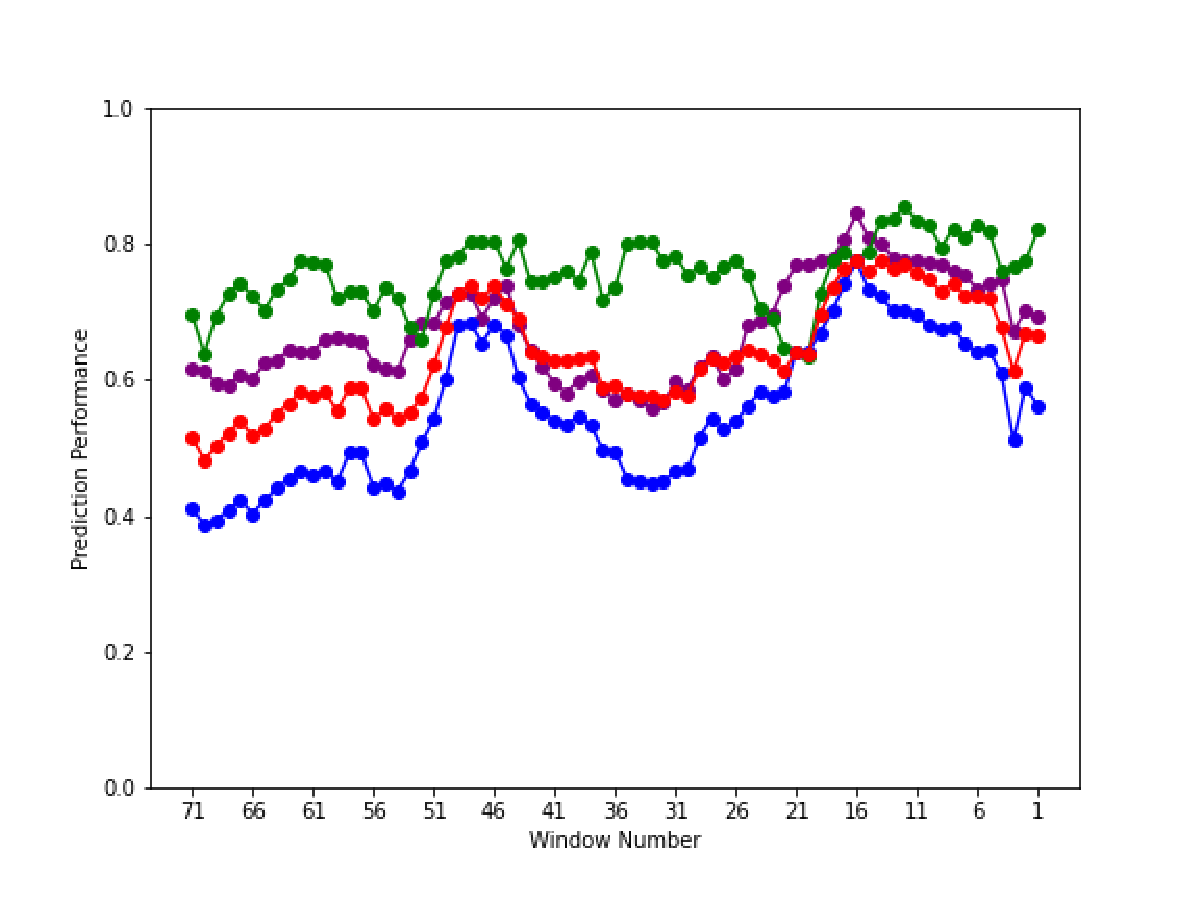
\includegraphics[width=0.495\textwidth]{Uenaka_fig/RQ1_result/review_Nova.pdf}
    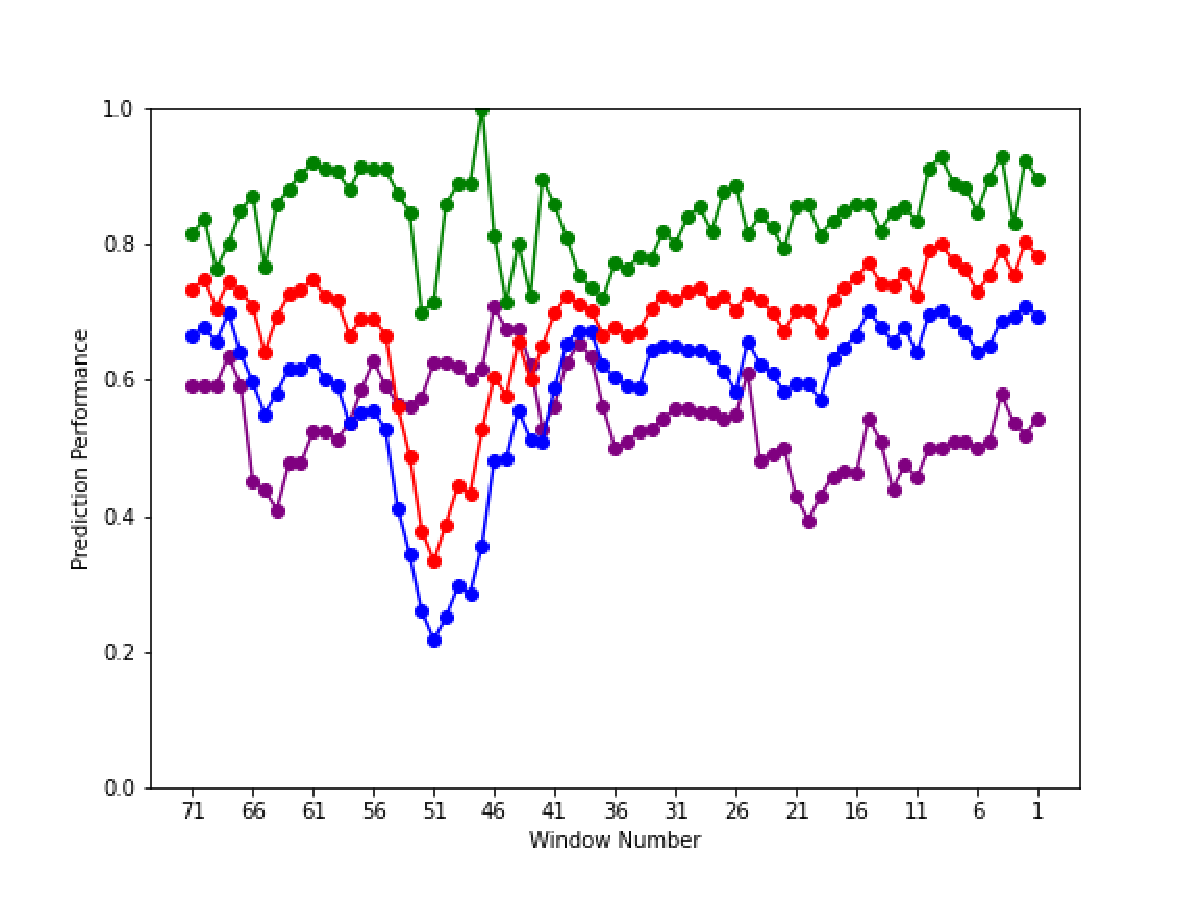
\includegraphics[width=0.495\textwidth]{Uenaka_fig/RQ1_result/review_Neutron.pdf}
    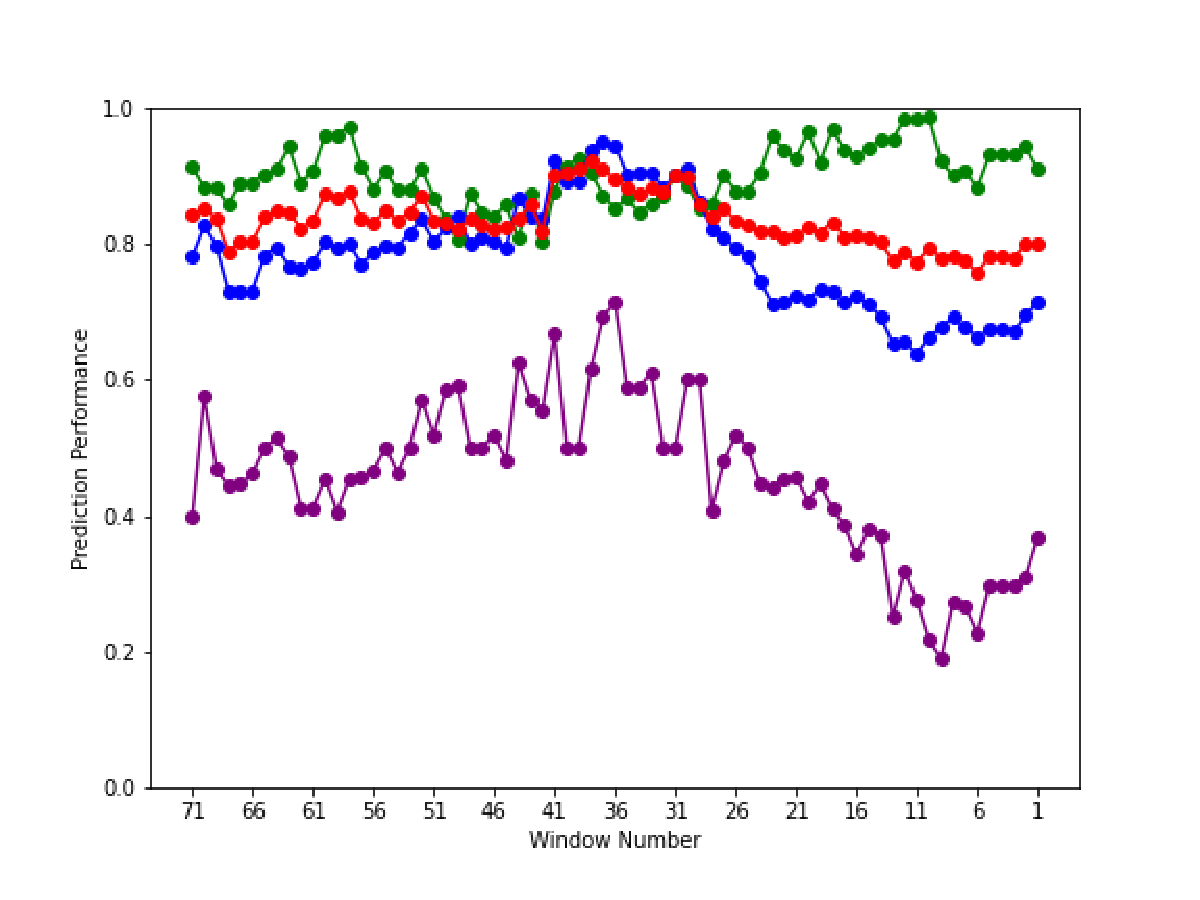
\includegraphics[width=0.495\textwidth]{Uenaka_fig/RQ1_result/review_Cinder.pdf}
    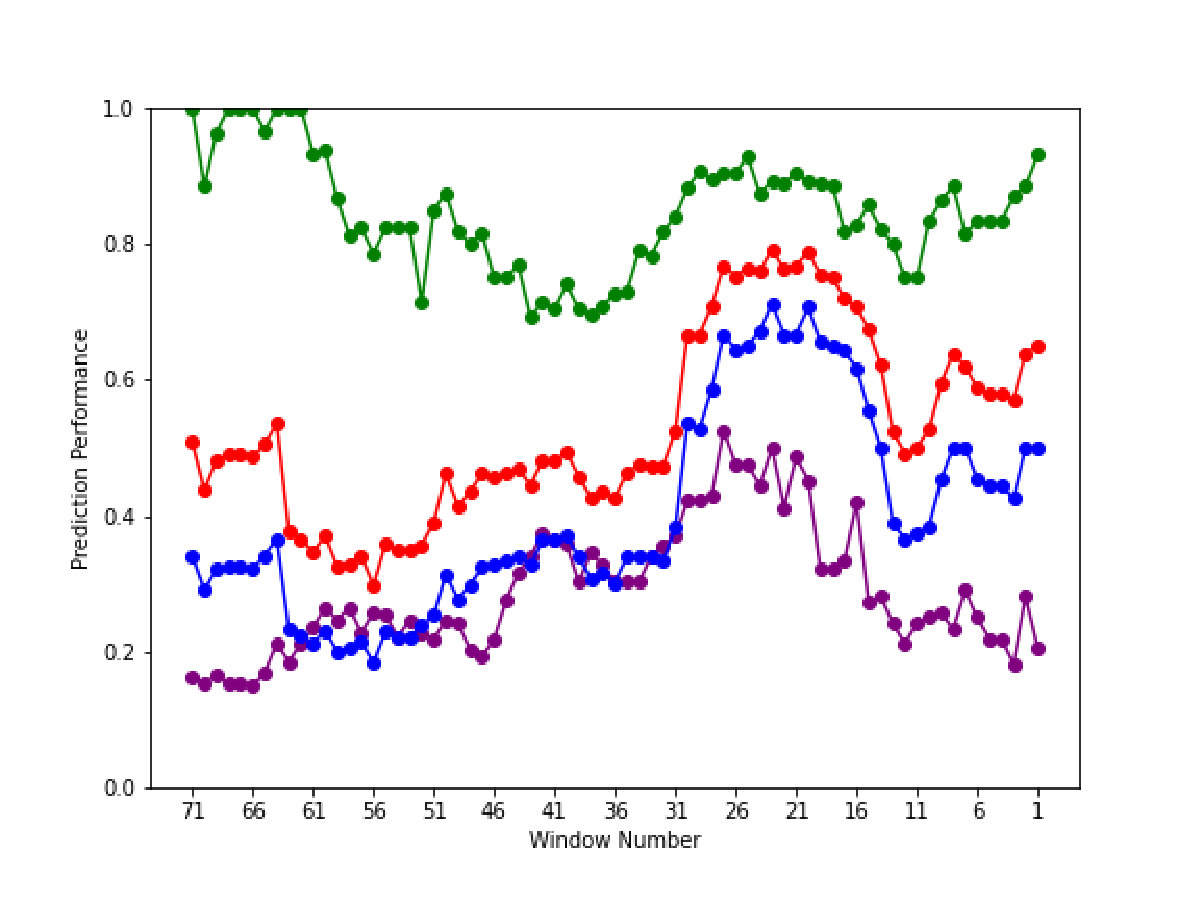
\includegraphics[width=0.495\textwidth]{Uenaka_fig/RQ1_result/review_Keystone.pdf}
    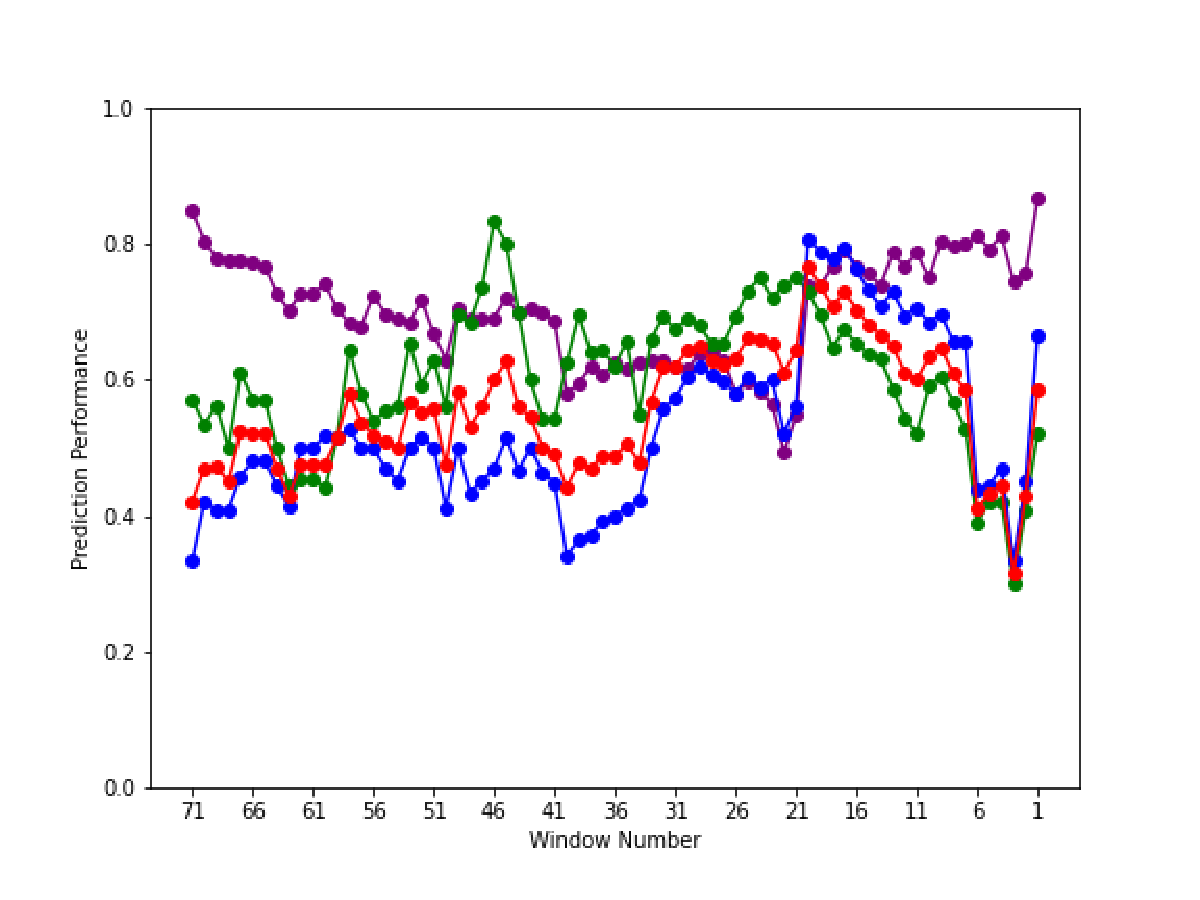
\includegraphics[width=0.495\textwidth]{Uenaka_fig/RQ1_result/review_Swift.pdf}
    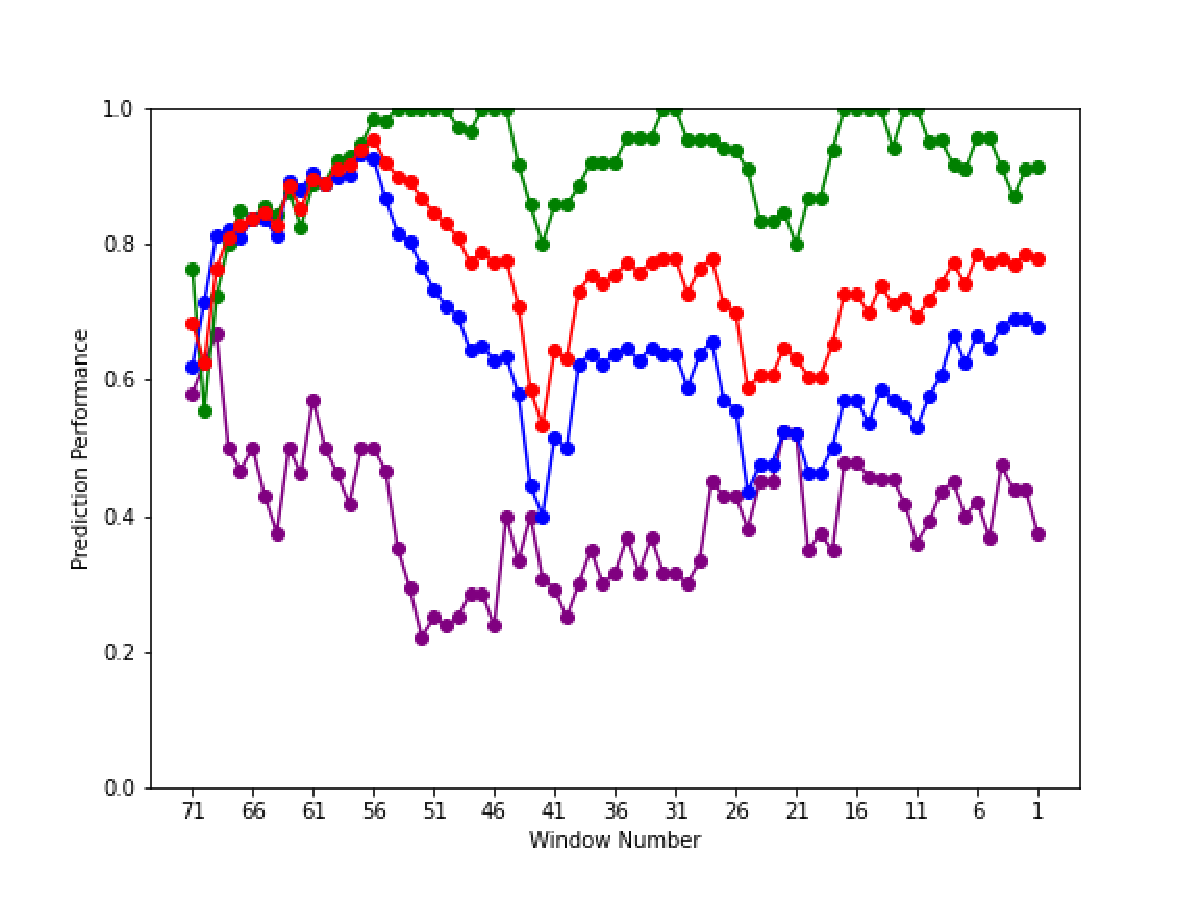
\includegraphics[width=0.495\textwidth]{Uenaka_fig/RQ1_result/review_Glance.pdf}
    \caption{レビュー予測モデルの予測性能(上段左:Nova,上段右:Neutron,中段左:Cinder,\\ 中段右:Keystone,下段左:Swift,下段右:Glance)(青:適合率,緑:再現率,紫:特異度,赤:F値)}
    \label{fig:review_base}
\end{center}
\end{figure}
%-----------------------


\subsection{マージ予測モデル}\label{sec:rq1_merge}
図\ref{fig:merge_base}は各プロジェクトにおけるベースラインモデルの予測性能を示す.図は横軸,縦軸や折れ線,図の配置は\ref{sec:rq1_review}項と同様である.なお,Glanceプロジェクトのウィンドウ71のみウィンドウ内の正例数が0であったため,本節における予測性能比較の対象外とする.また,表\ref{table:merge_hyoka_max}は各プロジェクトのマージ予測モデルにおける評価指標の範囲および差を示す.

表\ref{table:merge_hyoka_max}における予測性能の変動幅から,リリースまでの期間内において,従来手法の予測の正確性(適合率)は0.42〜0.83,正例の網羅率(再現率)は0.30〜0.95,負例の網羅率(特異度)は0.11〜0.16,予測性能(F値)は0.35〜0.48の変動幅で変化するという結果が得られた.次に評価指標ごとに結果を解釈する.

\textbf{(適合率)}0.42〜0.83の変動幅であるため,従来手法の適合率はリリースまでの期間内で大きく変化するという結果が得られた.

\textbf{(再現率およびF値)}Glanceプロジェクトを除き,それぞれ0.30〜0.43,0.35〜0.48の変動幅であり,最大値はそれぞれ0.33〜0.43,0.35〜0.48の低い水準で推移するという結果が得られた.

\textbf{(特異度)}0.11〜0.16と比較的小さい変動幅であり,最小値は0.81〜0.89と高止まりしているという結果が得られた.

本研究では,マージされるチケットとマージされないチケットの割合が不均衡であり,マージされないチケットが大半を占める.そのため,マージされるチケットの予測の正確性を評価する適合率はリリースまでの期間内で大きく変化し,マージされるチケットの網羅率を評価する再現率は低い水準で推移したと考えられる.これらの結果からF値に関しても低い水準で推移したと考えられる.また,マージされないチケットが大半を占めるデータセットであるため,マージされないチケットの網羅率を評価する特異度は高止まりしたと考えられる.
また,図\ref{fig:merge_base}の結果から,プロジェクトによって予測性能が高くなる時期は異なるものの,同一プロジェクトのバージョン間で優先的にマージされるチケットのチケットおよび開発者の特徴には共通性があることが示唆される.詳細については\ref{sec:rq1_kousatu1}節および\ref{sec:rq1_kousatu2}節で考察する.

\vskip\baselineskip
\fbox{\parbox{0.95\linewidth}{\textbf{(結果のまとめ)}マージされるチケットの予測において,従来手法の予測性能の変動幅は0.11〜0.95であり,リリースまでの期間内で大きく変化する.また,マージされるチケットとマージされないチケットの割合が不均衡であることが,予測性能に大きな影響を与えていると考えられる.}}

%--------------------
\begin{table*}[h]
\caption{マージ予測モデルにおける予測性能の範囲(最小値〜最大値)および変動幅}
\label{table:merge_hyoka_max}
\scalebox{0.65}{
\centering
\vspace{0.5zh}
\begin{tabular}{l|c|c|c|c|c|c}
    \hline \hline
    評価指標 & Nova & Neutron & Cinder & Keystone & Swift & Glance \\ \hline
    予測の正確性(適合率) & 0.02〜0.65 (0.63) & 0.0〜0.82 (0.82) & 0.0〜0.67 (0.67) & 0.17〜1.0 (0.83) & 0.0〜0.80 (0.80) & 0.08〜0.50 (0.42) \\ \hline
    正例の網羅率(再現率) & 0.14〜0.46 (0.32) & 0.0〜0.43 (0.43) & 0.0〜0.33 (0.33) & 0.03〜0.33 (0.30) & 0.0〜0.33 (0.33) & 0.05〜1.0 (0.95) \\ \hline
    負例の網羅率(特異度) & 0.85〜0.96 (0.11) & 0.83〜0.96 (0.13) & 0.85〜0.96 (0.11) & 0.89〜1.0 (0.11) & 0.82〜0.98 (0.16) & 0.81〜0.94 (0.13) \\ \hline
    予測性能(F値) & 0.04〜0.47 (0.43) & 0.0〜0.48 (0.48) & 0.0〜0.35 (0.35) & 0.05〜0.44 (0.39) & 0.0〜0.40 (0.40) & 0.07〜0.46 (0.39) \\ \hline
\end{tabular}
}
\end{table*}
%--------------------

%-----------------------
\begin{figure}[t]
\begin{minipage}{\textwidth}
\vspace{0.08\textheight}
\begin{center}
    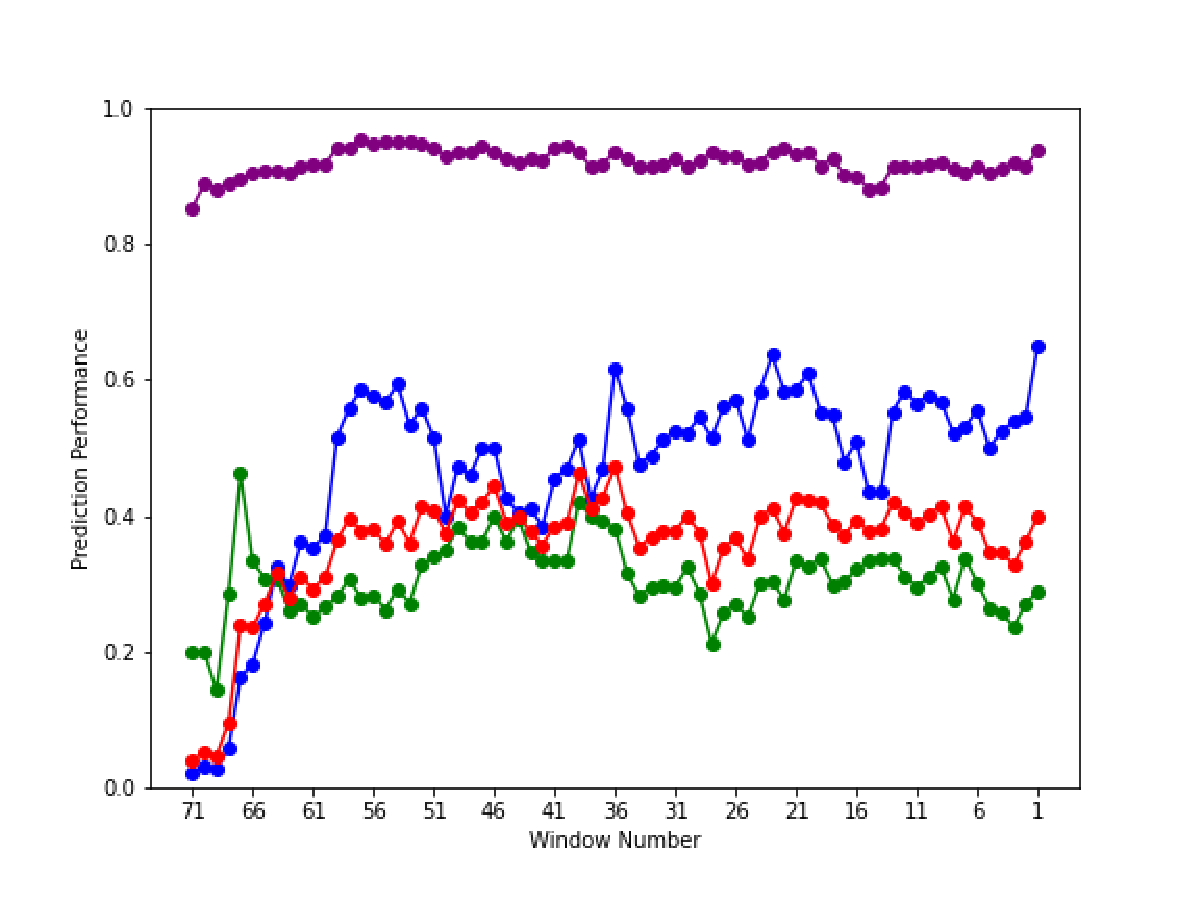
\includegraphics[width=0.495\textwidth]{Uenaka_fig/RQ1_result/merge_Nova.pdf}
    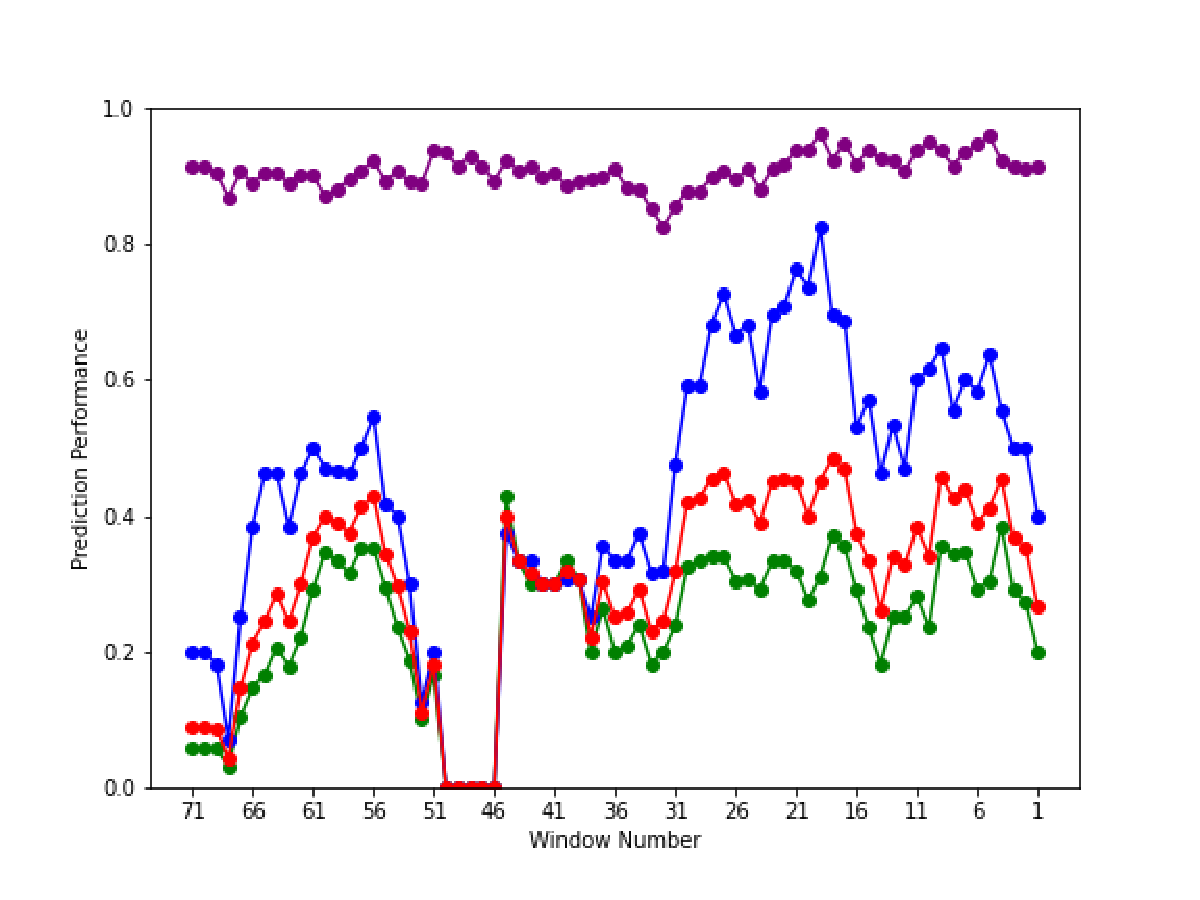
\includegraphics[width=0.495\textwidth]{Uenaka_fig/RQ1_result/merge_Neutron.pdf}
    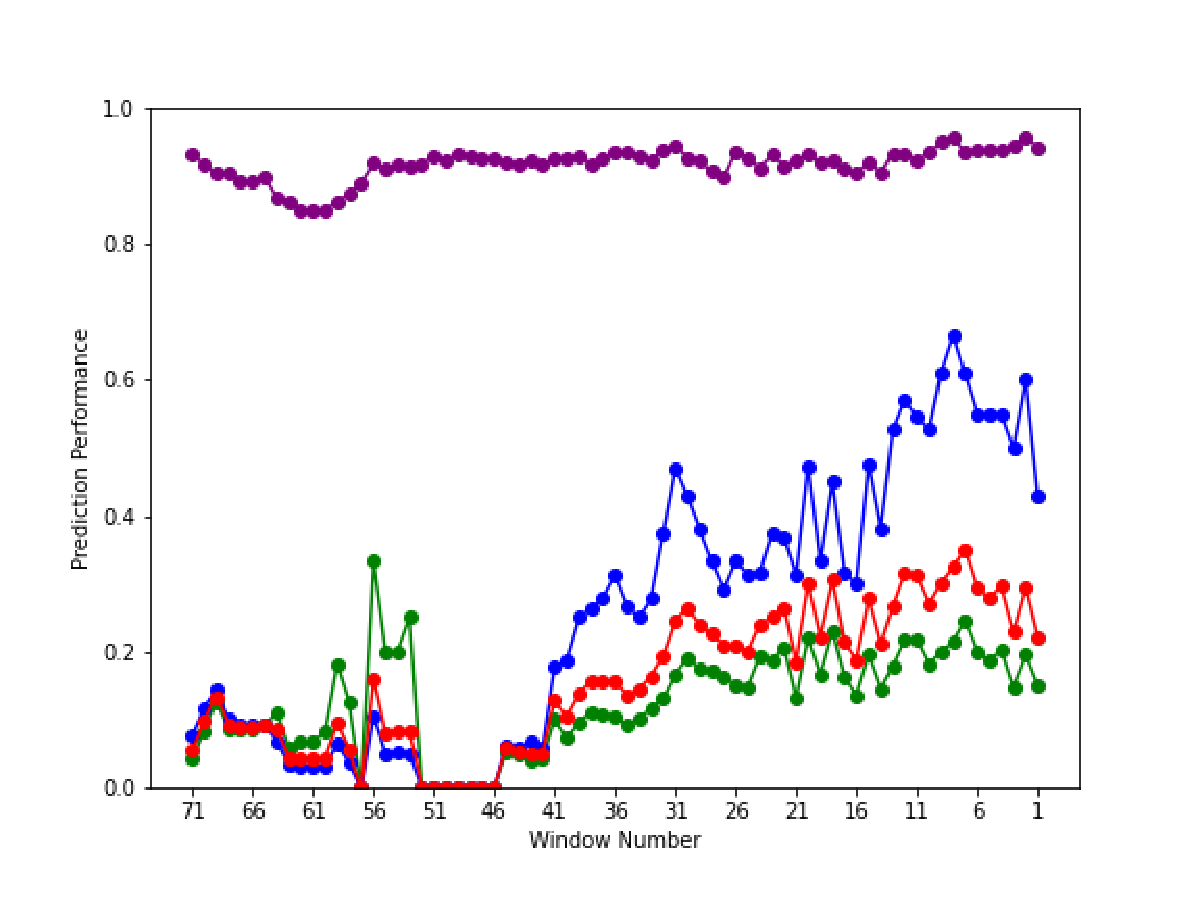
\includegraphics[width=0.495\textwidth]{Uenaka_fig/RQ1_result/merge_Cinder.pdf}
    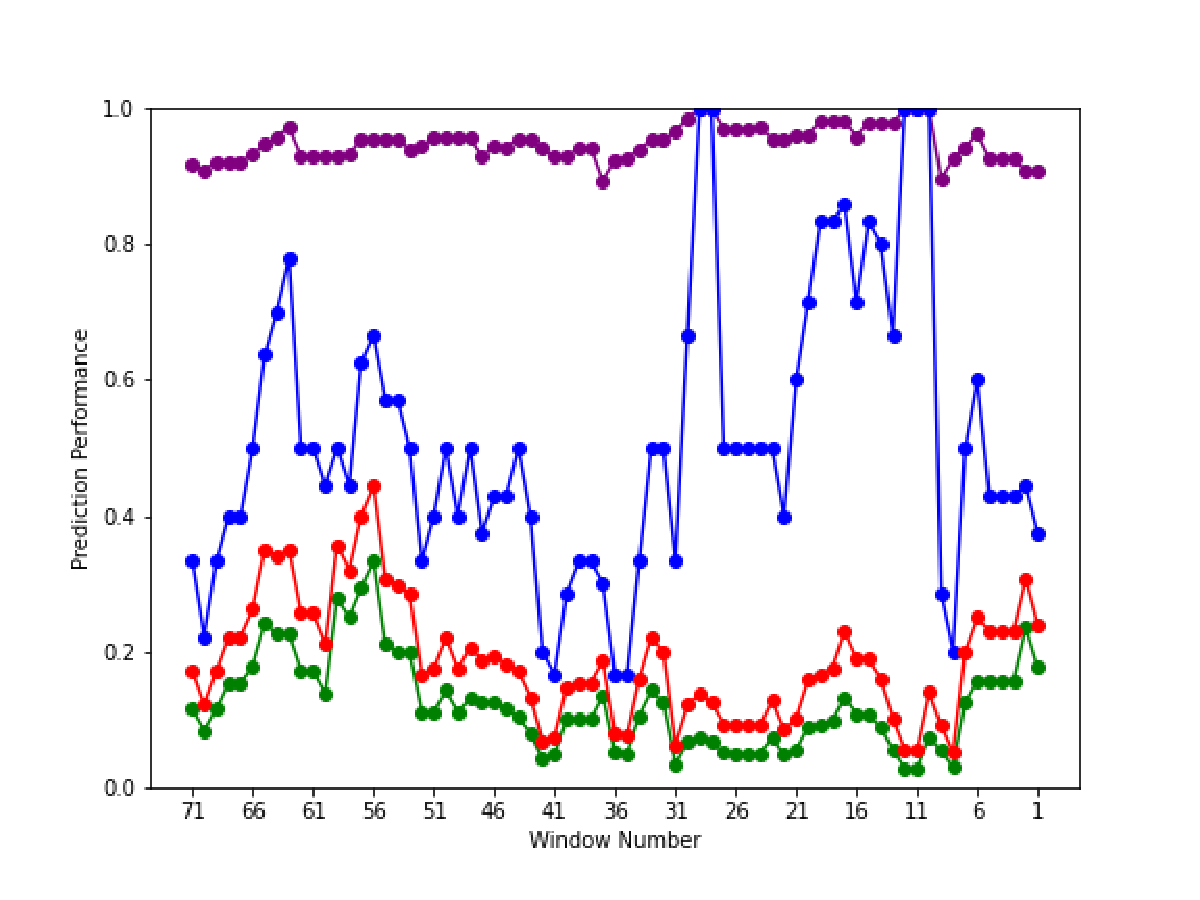
\includegraphics[width=0.495\textwidth]{Uenaka_fig/RQ1_result/merge_Keystone.pdf}
    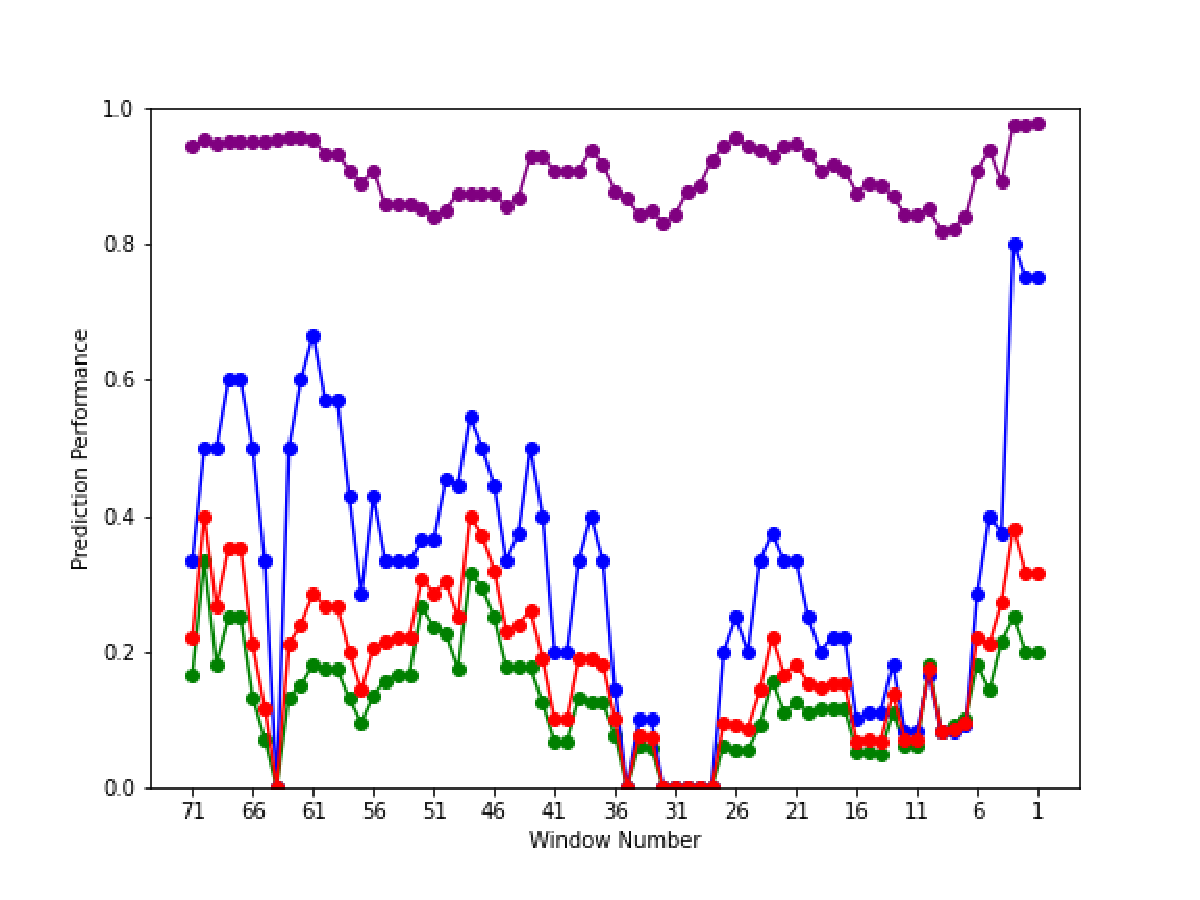
\includegraphics[width=0.495\textwidth]{Uenaka_fig/RQ1_result/merge_Swift.pdf}
    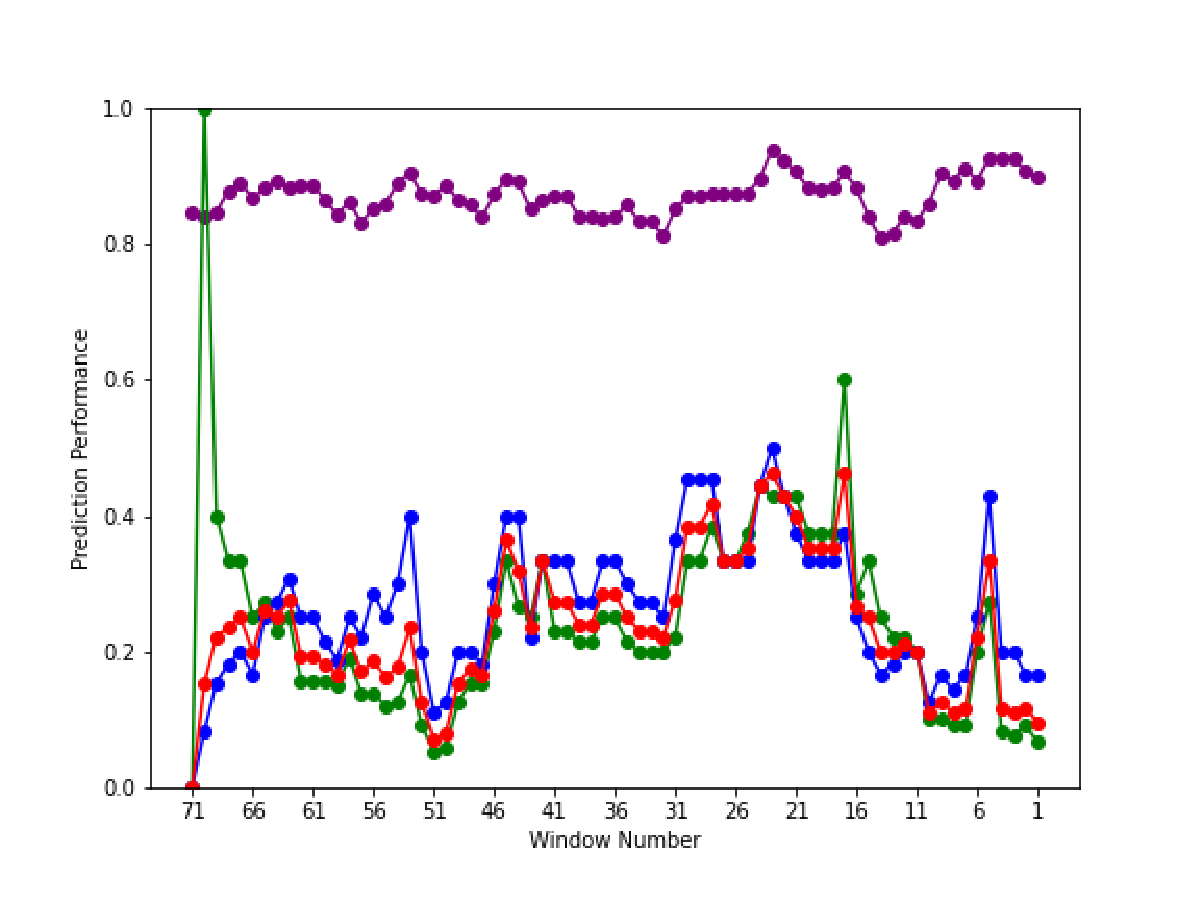
\includegraphics[width=0.495\textwidth]{Uenaka_fig/RQ1_result/merge_Glance.pdf}
    \caption{マージ予測モデルの予測性能(上段左:Nova,上段右:Neutron,中段左:Cinder,\\ 中段右:Keystone,下段左:Swift,下段右:Glance)(青:適合率,緑:再現率,紫:特異度,赤:F値)}
    \label{fig:merge_base}
\end{center}
\vspace{0.08\textheight}
\end{minipage}
\end{figure}
%-----------------------


\section{考察1:予測性能の時系列変化}\label{sec:rq1_kousatu1}
\ref{sec:rq1_result}節ではレビューが開始される/マージされるチケットの予測において,リリースまでの期間内でベースラインモデルの予測性能が大きく変化することを明らかにした.本節では,各評価指標について線形回帰分析を行うことで,リリースまでの期間内における予測性能の時系列変化から従来手法が有用となる時期を考察する.具体的には,各ウィンドウでの予測性能を$y$,各ウィンドウを$x$($x=72-N$)として回帰直線$y=a+bx$を計算することで回帰直線の傾き$b$(回帰係数)を求める.回帰係数が有意に増加または減少しているかに関してt検定を行い有意水準5\%で検定することで,各プロジェクトでのベースラインモデルの予測性能を以下の3つに分類する.

%-----------------------
\begin{itemize}
  \item \textbf{回帰係数が有意に増加する($b>0$,$P\text{値}<0.05$):}リリースが近づくにつれてベースラインモデルの予測性能が向上することを示す
  \item \textbf{回帰係数が有意に減少する($b<0$,$P\text{値}<0.05$):}リリースが近づくにつれてベースラインモデルの予測性能が低下することを示す
  \item \textbf{回帰係数が有意に増加および減少しない($P\text{値}>0.05$):}リリース時期によってベースラインモデルの予測性能が変化しない(一定である)ことを示す
\end{itemize}
%-----------------------

\subsection{レビュー予測モデル}
表\ref{table:review_seino_jikeiretsu}はベースラインモデルの予測性能の時系列変化の分析結果として,各プロジェクトのレビュー予測モデルにおける評価指標の回帰係数の分類を示す.表\ref{table:review_seino_jikeiretsu}において,回帰係数が有意に増加する場合は『$\nearrow$』,回帰係数が有意に減少する場合は『$\searrow$』,回帰係数が有意に増加および減少しない場合は『$\rightarrow$』で表す.

表\ref{table:review_seino_jikeiretsu}の結果から,共通の傾向をもつプロジェクトごとに結果を考察する.

\textbf{(全ての評価指標が向上もしくは一定)}Nova,Keystone,Swiftプロジェクトでは,ベースラインモデルの全ての評価指標がリリースが近づくにつれて向上もしくはリリース時期に関わらず一定であった.この結果から,これらのプロジェクトではリリースが近づくにつれて,チケットおよび開発者の特徴からチケットのレビューを開始するか否かを判断する傾向にあることが示唆される.
% 従来手法はリリースが近づくにつれて有用であると考えられる.このことから,

\textbf{ (正例の評価指標は向上もしくは一定であり,負例の評価指標は低下) }Neutronプロジェクトでは,ベースラインモデルの正例の評価指標はリリースが近づくにつれて向上もしくはリリース時期に関わらず一定であり,負例の評価指標は低下した.この結果から,Neutronプロジェクトでは,リリースが近づくにつれてチケットおよび開発者の特徴からレビューを開始するチケットを判断する傾向にあり,リリースが遠いほどチケットおよび開発者の特徴からレビューを開始しないチケットを判断する傾向にあることが示唆される.
% そのためNeutronプロジェクトでは,従来手法は正例の検出に関してはリリースが近づくにつれて有用であり,負例の検出に関してはリリースが遠いほど有用であると考えられる.

\textbf{(適合率およびF値が低下)}Cinder,Glanceプロジェクトでは,リリースが近づくにつれてベースラインモデルの適合率およびF値が低下した.この結果から,これらのプロジェクトではリリースが遠いほど,チケットおよび開発者の特徴からレビューを開始するチケットを判断する傾向にあることが示唆される.
% 従来手法はリリースが遠いほど有用であると考えられる.

これらの結果から,従来手法の予測性能の時系列変化の傾向は3種類に大別されることを明らかにした.\ref{sec:rq1_kousatu2}節では,これらの結果を踏まえ,ベースラインモデルで予測性能が高い時期のチケットの特徴量から予測性能が向上した理由を考察する.
% 従来手法が有用となる時期は複数の傾向に大別されることを明らかにした.


%--------------------
\begin{table*}[t]
\caption{各プロジェクトのレビュー予測モデルにおける評価指標の回帰係数の分類}
\label{table:review_seino_jikeiretsu}
\centering
\vspace{0.5zh}
\scalebox{0.9}{
\begin{tabular}{l|c|c|c|c|c|c}
    \hline \hline
    評価指標 & Nova & Neutron & Cinder & Keystone & Swift & Glance \\ \hline
    適合率 & $\nearrow$ & $\nearrow$ & $\searrow$ & $\nearrow$ & $\nearrow$ & $\searrow$ \\ \hline
    再現率 & $\nearrow$ & $\rightarrow$ & $\nearrow$ & $\rightarrow$ & $\rightarrow$ & $\nearrow$ \\ \hline
    特異度 & $\nearrow$ & $\searrow$ & $\searrow$ & $\nearrow$ & $\rightarrow$ & $\rightarrow$ \\ \hline
    F値 & $\nearrow$ & $\nearrow$ & $\searrow$ & $\nearrow$ & $\nearrow$ & $\searrow$ \\ \hline
\end{tabular}}
\end{table*}
%--------------------



\subsection{マージ予測モデル}
表\ref{table:merge_seino_jikeiretsu}はベースラインモデルの予測性能の時系列変化の分析結果として,各プロジェクトのマージ予測モデルにおける評価指標の回帰係数の分類を示す.表\ref{table:merge_seino_jikeiretsu}において,回帰係数の分類は表\ref{table:review_seino_jikeiretsu}と同様の矢印で表す.

表\ref{table:merge_seino_jikeiretsu}の結果から,共通の傾向をもつプロジェクトごとに結果を考察する.
% リリースが近づくにつれて,全ての評価指標は2プロジェクト (Neutron, Cinder) で向上し,2プロジェクト (Nova, Glance) で向上もしくは一定であるという結果が得られた.また,2プロジェクト (Keystone, Swift) では再現率およびF値が低下するという結果が得られた.

\textbf{(全ての評価指標が向上)}Neutron,Cinderプロジェクトでは,リリースが近づくにつれてベースラインモデルの全ての評価指標が向上した.この結果から,これらのプロジェクトではリリースが近づくにつれて,チケットおよび開発者の特徴からチケットをマージするか否かを判断する傾向にあることが示唆される.
% 従来手法はリリースが近づくにつれて有用であると考えられる.このことから,

\textbf{ (正例の評価指標は向上もしくは一定であり,負例の評価指標は一定) }Novaプロジェクトでは,ベースラインモデルの正例の評価指標はリリースが近づくにつれて向上もしくはリリース時期に関わらず一定であり,負例の評価指標はリリース時期に関わらず一定であった.この結果から,Novaプロジェクトでは,リリースが近づくにつれてチケットおよび開発者の特徴からマージするチケットを判断する傾向にあることが示唆される.
% そのため,Novaプロジェクトでは従来手法は,正例の検出に関してはリリースが近づくにつれて有用であると考えられる.

\textbf{ (負例の評価指標は向上し,正例の評価指標は一定である) }Glanceプロジェクトでは,リリースが近づくにつれてベースラインモデルの負例の評価指標は向上し,正例の評価指標はリリース時期に関わらず一定であった.この結果から,Glanceプロジェクトでは,リリースが近づくにつれてチケットおよび開発者の特徴からマージしないチケットを判断する傾向にあることが示唆される.
% そのため,Glanceプロジェクトでは従来手法は,負例の検出に関してはリリースが近づくにつれて有用であると考えられる.

\textbf{(再現率およびF値が低下)}Keystone,Swiftプロジェクトでは,リリースが近づくにつれてベースラインモデルの再現率およびF値が低下した.この結果から,これらのプロジェクトではリリースが遠いほど,チケットおよび開発者の特徴からマージするチケットを判断する傾向にあることが示唆される.
% 従来手法はリリースが遠いほど有用であると考えられる.

これらの結果から,従来手法の予測性能の時系列変化の傾向は4種類に大別されることを明らかにした.そこで,マージ予測モデルに関しても,\ref{sec:rq1_kousatu2}節で予測性能が向上した理由を考察する.

%--------------------
\begin{table*}[t]
\caption{各プロジェクトのマージ予測モデルにおける評価指標の回帰係数の分類}
\label{table:merge_seino_jikeiretsu}
\centering
\vspace{0.5zh}
\scalebox{0.9}{
\begin{tabular}{l|c|c|c|c|c|c}
    \hline \hline
    評価指標 & Nova & Neutron & Cinder & Keystone & Swift & Glance \\ \hline
    適合率 & $\nearrow$ & $\nearrow$ & $\nearrow$ & $\nearrow$ & $\searrow$ & $\rightarrow$ \\ \hline
    再現率 & $\rightarrow$ & $\nearrow$ & $\nearrow$ & $\searrow$ & $\searrow$ & $\rightarrow$ \\ \hline
    特異度 & $\rightarrow$ & $\nearrow$ & $\nearrow$ & $\nearrow$ & $\rightarrow$ & $\nearrow$ \\ \hline
    F値 & $\nearrow$ & $\nearrow$ & $\nearrow$ & $\searrow$ & $\searrow$ & $\rightarrow$ \\ \hline
\end{tabular}}
\end{table*}
%--------------------


\section{考察2:予測性能の向上理由}\label{sec:rq1_kousatu2}
本節では,ベースラインモデルの予測性能が高い時期における正例のチケットの特徴量を分析することで,ベースラインモデルの予測性能が向上した理由を考察する.具体的には,従来研究\cite{shap}で提案されたSHAP (SHapley Additive exPlanations) の中でも決定木ベースの機械学習モデル用に最適化されたTree SHAP(後の研究\cite{TreeSHAP}で詳細化)を用いて各説明変数の重要度を算出する.Tree SHAPでは,各テストケースの予測においてそれぞれの説明変数が正負どちらの方向にどの程度寄与したかを重要度として出力する.本節では正例のチケットに着目し,正の方向に寄与した説明変数の重要度を分析する.分析にあたっては,\ref{sec:rq1_kousatu1}節の表\ref{table:review_seino_jikeiretsu}および表\ref{table:merge_seino_jikeiretsu}におけるF値の結果を元に以下に示すウィンドウを抽出する.そして,当該ウィンドウの正例のチケットについて重要度を算出し,各チケットにおける重要度の平均をとることで,予測性能が高い時期の正例のチケットの予測において重要となった説明変数を明らかにする.

%-----------------------
\begin{itemize}
  \item \textbf{リリースが近づくにつれてF値が向上したプロジェクト:}リリース後半のウィンドウ(ウィンドウ1〜36)の中で最もF値の高いウィンドウ
  \item \textbf{リリースが近づくにつれてF値が低下したプロジェクト:}リリース前半のウィンドウ(ウィンドウ36〜71)の中で最もF値の高いウィンドウ
  \item \textbf{リリース時期に関わらずF値が一定であるプロジェクト:}全ウィンドウ(ウィンドウ1〜71)の中で最もF値の高いウィンドウ
\end{itemize}
%-----------------------

また,当該ウィンドウで重要度の高い説明変数について,正例/負例間に統計的有意差があるか否かを検定し,正例/負例間の説明変数の違いを分析することで,ベースラインモデルの予測性能が向上した理由を考察する.
統計検定手法には\ref{sec:pre_analysis}章同様,比例尺度の説明変数に対してはマンホイットニーのU検定,名義尺度の説明変数に対してはカイ2乗検定を用いてP値を算出することで,統計的有意差の有無を検定する.


\subsection{レビュー予測モデル}\label{sec:rq1_kousatu2_review}
表\ref{table:review_importance}は,各プロジェクトで抽出したウィンドウにおいて,レビューが開始されるチケットの予測で重要度の高い説明変数と重要度を示す.

表\ref{table:review_importance}から,全てのプロジェクトで経過時間が最も重要度の高い説明変数であるという結果が得られた.また,報告実績やマージ実績といった開発者の特徴や追加行数やバグ修正確信度といったチケットの特徴が経過時間の次に重要度の高い説明変数であるという結果が得られた.

\begin{table}[t]
\caption{レビューが開始されるチケットの予測において重要度の高い説明変数と重要度}
\label{table:review_importance}
\centering
\vspace{0.5zh}
\scalebox{0.88}{
\begin{tabular}{l|c|cc|cc|cc}
    \hline \hline
    \multirow{2}{*}{プロジェクト}   & \multicolumn{1}{l|}{\multirow{2}{*}{ウィンドウ}} & \multicolumn{2}{c|}{1位} & \multicolumn{2}{c|}{2位} & \multicolumn{2}{c}{3位}  \\ \cline{3-8}
    & \multicolumn{1}{c|}{}  & 説明変数名 & \multicolumn{1}{c|}{重要度} & 説明変数名 & \multicolumn{1}{c|}{重要度} & 説明変数名 & \multicolumn{1}{c}{重要度} \\ \hline
    Nova  & 16  & 経過時間  & 0.20 & 報告実績  & 0.03  & バグ修正確信度 & 0.03  \\
    Neutron  & 2  & 経過時間  & 0.15  & バグ修正確信度  & 0.06 & 追加行数 & 0.04  \\
    Cinder   & 37  & 経過時間  & 0.17  & バグ修正確信度  & 0.06  & 追加行数 & 0.05  \\
    Keystone & 23  & 経過時間  & 0.16  & バグ修正確信度  & 0.04  & 追加行数 & 0.04  \\
    Swift    & 20  & 経過時間  & 0.15  & 追加行数  & 0.05  & 報告実績 & 0.05  \\
    Glance   & 56  & 経過時間  & 0.10  & マージ実績  & 0.08  & 追加行数  & 0.06  \\ \hline
\end{tabular}}
\end{table}

表\ref{table:review_importance_yuisa}は,表\ref{table:review_importance}のそれぞれの説明変数についてレビューが開始されるチケット(正例)とレビューが開始されないチケット(負例)の間に有意差があるか(P値 $<$ 0.05)および有意差のある説明変数の正例と負例の違いを示す.説明変数の正例と負例の違いとして,比例尺度の説明変数に関しては,正例の方が値が大きくなる場合$\nearrow$,値が小さくなる場合$\searrow$で表す.また,名義尺度の説明変数(バグ修正確信度)に関しては,バグ修正確信度の高いチケットの割合が増加した場合$\nearrow$,バグ修正確信度の高いチケットの割合が減少した場合$\searrow$で表す.

表\ref{table:review_importance_yuisa}から,経過時間はKeystoneプロジェクト以外の全てのプロジェクトで正例と負例の間で有意差があり,正例の方が値が小さくなるという結果が得られた.この結果から,レビューが開始されるチケットの中でも経過時間の短いチケットに対して,正しくレビューが開始されると予測したことで従来手法の予測性能が向上したことが示唆される.

また,Nova,Neutronプロジェクトでは,経過時間の他にバグ修正確信度について,正例と負例の間で有意差があるという結果が得られた.それぞれの傾向として,Novaプロジェクトではバグ修正確信度の高いチケットの割合が減少し,Neutronプロジェクトではバグ修正確信度の高いチケットの割合が増加した.この結果から,Novaプロジェクトではバグ修正でないチケットをレビューする傾向にあり,レビューが開始されるチケットの中でもバグ修正でないチケットに対して,正しくレビューが開始されると予測したことで従来手法の予測性能が向上したことが示唆される.一方Neutronプロジェクトではバグ修正のチケットをレビューする傾向にあり,レビューが開始されるチケットの中でもバグ修正のチケットに対して,正しくレビューが開始されると予測したことで従来手法の予測性能が向上したことが示唆される.

また,Glanceプロジェクトでは,経過時間の他にマージ実績について,正例と負例の間で有意差があり,正例の方が値が大きくなるという結果が得られた.この結果から,レビューが開始されるチケットの中でもマージ実績の高い開発者の報告したチケットに対して,正しくレビューが開始されると予測したことで従来手法の予測性能が向上したことが示唆される.

% \vskip\baselineskip
% \fbox{\parbox{0.95\linewidth}{\textbf{(結果のまとめ)}レビューが開始されるチケットの予測において,全てのプロジェクトで経過時間が最も正例の判別に寄与した.また,経過時間の短いチケットについてレビューが開始されると予測したことで,従来手法の予測性能が向上したと考えられる.}}

\begin{table}[t]
\caption{レビュー予測モデルにおいて重要度の高い説明変数の正例と負例の有意差および違い}
\label{table:review_importance_yuisa}
\centering
\vspace{0.5zh}
\scalebox{0.73}{
\begin{tabular}{l|c|ccc|ccc|ccc}
    \hline \hline
    \multirow{2}{*}{プロジェクト} & \multicolumn{1}{l|}{\multirow{2}{*}{ウィンドウ}} & \multicolumn{3}{c|}{1位}  & \multicolumn{3}{c|}{2位}  & \multicolumn{3}{c}{3位} \\ \cline{3-11}
     & \multicolumn{1}{c|}{} & 説明変数名 & 有意差 & \multicolumn{1}{c|}{違い} & \multicolumn{1}{c}{説明変数名} & 有意差 & \multicolumn{1}{c|}{違い} & \multicolumn{1}{c}{説明変数名} & 有意差 & \multicolumn{1}{c}{違い} \\ \hline
    Nova & 16 & 経過時間  & 有  & $\searrow$  & 報告実績  & 無  & - & バグ修正確信度  & 有  & $\searrow$   \\
    Neutron & 2 & 経過時間  & 有  & $\searrow$ & バグ修正確信度  & 有 & $\nearrow$ & 追加行数  & 無  &  -  \\
    Cinder & 37 & 経過時間  & 有   & $\searrow$ & バグ修正確信度  & 無 & - & 追加行数  & 無 &  -   \\
    Keystone & 23 & 経過時間  & 無 & - & バグ修正確信度  & 無 & - & 追加行数  & 無 &  -   \\
    Swift & 20 & 経過時間  & 有 &  $\searrow$  & 追加行数  & 無 &  -  & 報告実績   & 無 &  -     \\
    Glance & 56 & 経過時間  & 有 & $\searrow$ & マージ実績  & 有 & $\nearrow$ & 追加行数  & 無 &  -   \\ \hline
\end{tabular}}
\end{table}


\subsection{マージ予測モデル}
表\ref{table:merge_importance}は,各プロジェクトで抽出したウィンドウにおいて,マージされるチケットの予測で重要度の高い説明変数と重要度を示す.

表\ref{table:merge_importance}から,マージされるチケットの予測に関しても,全てのプロジェクトで経過時間が最も重要度の高い説明変数であるという結果が得られた.また,Swiftプロジェクトを除く5プロジェクトでは追加行数が経過時間の次に重要度の高い説明変数であるという結果が得られ,Swiftプロジェクトにおいても報告実績の次に重要度の高い説明変数であった.その他には報告実績や直近報告実績,マージ実績といった開発者の特徴やバグ修正確信度といったチケットの特徴が重要度の高い説明変数であるという結果が得られた.

\begin{table}[t]
\caption{マージが開始されるチケットの予測において重要度の高い説明変数と重要度}
\label{table:merge_importance}
\centering
\vspace{0.5zh}
\scalebox{0.88}{
\begin{tabular}{l|c|cc|cc|cc}
    \hline \hline
    \multirow{2}{*}{プロジェクト}   & \multicolumn{1}{l|}{\multirow{2}{*}{ウィンドウ}} & \multicolumn{2}{c|}{1位} & \multicolumn{2}{c|}{2位} & \multicolumn{2}{c}{3位}  \\ \cline{3-8}
    & \multicolumn{1}{c|}{}  & 説明変数名 & \multicolumn{1}{c|}{重要度} & 説明変数名 & \multicolumn{1}{c|}{重要度} & 説明変数名 & \multicolumn{1}{c}{重要度} \\ \hline
    Nova  & 36  & 経過時間  & 0.12 & 追加行数  & 0.05  & 直近報告実績 & 0.04  \\
    Neutron  & 18  & 経過時間  & 0.08  & 追加行数  & 0.06 & マージ実績 & 0.03  \\
    Cinder   & 7  & 経過時間  & 0.10  & 追加行数  & 0.05  & 報告実績 & 0.05  \\
    Keystone & 56  & 経過時間  & 0.11  & 追加行数  & 0.04  & 報告実績 & 0.03  \\
    Swift    & 48  & 経過時間  & 0.12  & 報告実績  & 0.05  & 追加行数 & 0.03  \\
    Glance   & 23  & 経過時間  & 0.14  & 追加行数  & 0.06  & バグ修正確信度 & 0.05  \\ \hline
\end{tabular}}
\end{table}


表\ref{table:merge_importance_yuisa}は,表\ref{table:merge_importance}のそれぞれの説明変数についてマージされるチケット(正例)とマージされないチケット(負例)の間に有意差があるか(P値 $<$ 0.05)および有意差のある説明変数の正例と負例の違いを示す.説明変数の正例と負例の違いの表し方は\ref{sec:rq1_kousatu2_review}項と同様である.

表\ref{table:merge_importance_yuisa}から,経過時間はNeutronプロジェクト以外の全てのプロジェクトで正例と負例の間で有意差があり,正例の方が値が小さくなるという結果が得られた.この結果から,マージされるチケットの中でも経過時間の短いチケットに対して,正しくマージされると予測したことで従来手法の予測性能が向上したことが示唆される.

また,Nova,Neutronプロジェクトでは,経過時間の他に追加行数について,正例と負例の間で有意差があり,正例の方が追加行数が少なくなるという結果が得られた.この結果から,マージされるチケットの中でも追加行数の少ないチケットに対して,正しくマージされると予測したことで従来手法の予測性能が向上したことが示唆される.

また,Nova,Cinderプロジェクトでは,直近報告実績,報告実績のような開発者の特徴について,正例と負例の間で有意差があり,正例の方が値が大きくなるという結果が得られた.この結果から,マージされるチケットの中でも直近報告実績や報告実績の高い開発者の報告したチケットに対して,正しくマージされると予測したことで従来手法の予測性能が向上したことが示唆される.


\begin{table}[t]
\caption{マージ予測モデルにおいて重要度の高い説明変数の正例と負例の有意差および違い}
\label{table:merge_importance_yuisa}
\centering
\vspace{0.5zh}
\scalebox{0.73}{
\begin{tabular}{l|c|ccc|ccc|ccc}
    \hline \hline
    \multirow{2}{*}{プロジェクト} & \multicolumn{1}{l|}{\multirow{2}{*}{ウィンドウ}} & \multicolumn{3}{c|}{1位}  & \multicolumn{3}{c|}{2位}  & \multicolumn{3}{c}{3位} \\ \cline{3-11}
     & \multicolumn{1}{c|}{} & 説明変数名 & 有意差 & \multicolumn{1}{c|}{違い} & \multicolumn{1}{c}{説明変数名} & 有意差 & \multicolumn{1}{c|}{違い} & \multicolumn{1}{c}{説明変数名} & 有意差 & \multicolumn{1}{c}{違い} \\ \hline
    Nova & 36 & 経過時間  & 有 & $\searrow$ & 追加行数  & 有 & $\searrow$ & 直近報告実績 & 有 & $\nearrow$  \\
    Neutron & 18 & 経過時間  & 無 & - & 追加行数  & 有   & $\searrow$  & マージ実績  & 無   &  -  \\
    Cinder & 7 & 経過時間  & 有  & $\searrow$ & 追加行数  & 無   & - & 報告実績  & 有   &  $\nearrow$   \\
    Keystone & 56 & 経過時間  & 有   &  $\searrow$ & 追加行数  & 無 & - & 報告実績  & 無 &  -   \\
    Swift & 48 & 経過時間  & 有   &  $\searrow$  & 報告実績  & 無 &  -  & 追加行数   & 無   &  -     \\
    Glance & 23 & 経過時間  & 有 & $\searrow$ & 追加行数  & 無 & - & バグ修正確信度  & 無 &  -   \\ \hline
\end{tabular}}
\end{table}


\section{RQ1のまとめ}\label{sec:rq1_matome}
本節では,\ref{sec:rq1_result}節,\ref{sec:rq1_kousatu1}節,\ref{sec:rq1_kousatu2}節の結果からRQ1の結果をまとめる.

\ref{sec:rq1_result}節の結果から,従来手法の予測性能の変動幅は,レビューが開始されるチケットの予測において0.16〜0.53,マージされるチケットの予測において0.11〜0.95であり,リリースまでの期間内で大きく変化する.また,図\ref{fig:review_base}および図\ref{fig:merge_base}の結果から,プロジェクトによって予測性能が高くなる時期は異なるものの,同一プロジェクトのバージョン間で優先されるチケットのチケットおよび開発者の特徴には共通性があることが示唆された.

\ref{sec:rq1_kousatu1}節では考察として,予測性能の時系列変化を分析した.結果として,従来手法の予測性能の時系列変化の傾向は3種類から4種類に大別できる.そこで,\ref{sec:rq1_kousatu2}節では従来手法の予測性能が高い時期において重要度の高い特徴量を明らかにすることで,予測性能が向上した理由を考察した.結果として,レビュー予測モデル,マージ予測モデルともに全てのプロジェクトで経過時間が最も重要度が高く,負例のチケットに比べ正例のチケットの経過時間が短いことを明らかにした.この結果から,全てのプロジェクトにおいて,レビュアは経過時間の短いチケットの優先順位を高く見積もる傾向にあることが示唆される.
また,従来手法の予測性能が高い時期においては,経過時間の短い正例のチケットを正しく正例と判別することで従来手法の予測性能は向上したと考えられる.


%%%%%%%%%%%%%%%%%%%%%%%%%%%%%%%%%
\section{RQ2:\rqtwo}\label{sec:rq2}
%%%%%%%%%%%%%%%%%%%%%%%%%%%%%%%%%
RQ2では,提案モデルとベースラインモデルの予測性能を比較し,開発状況に関する説明変数を用いることで,予測性能はリリースまでの期間によってどの程度変化するかを明らかにする.

\section{予測結果}\label{sec:rq2_result}
\subsection{レビュー予測モデル}\label{sec:rq2_review}
レビュー予測モデルの予測結果として,図\ref{fig:review_p}は適合率,図\ref{fig:review_r}は再現率,図\ref{fig:review_spec}は特異度,図\ref{fig:review_f}はF値を示す.図は横軸が各ウィンドウ,縦軸が予測性能を表しており,赤の折れ線が提案モデルの予測性能,青の折れ線がベースラインモデルの予測性能を表す.また,図の左から右に向かってリリースに近いウィンドウ(最も左はウィンドウ71,最も右はウィンドウ1)での予測結果を表す.図\ref{fig:review_p}から図\ref{fig:review_f}までの各プロジェクトにおいて,7つ以上の連続したウィンドウ(3週間以上の期間)において提案モデルの予測性能がベースラインモデルの予測性能と比べて向上した期間(向上期間)を赤色,低下した期間(低下期間)を青色で表している.また,図\ref{fig:review_prepare_P}から図\ref{fig:review_prepare_F}は図\ref{fig:review_p}から図\ref{fig:review_f}の結果に基づき,各プロジェクトにおける向上期間を赤色,低下期間を青色の矢印で示している.また,各矢印上の数値は当該期間における提案モデルとベースラインモデルの予測性能の差の平均値を示し,右端にはリリースまでの全期間における提案モデルとベースラインモデルの予測性能の差の平均値を示す.また,結果の解釈のためにリリースまでの期間を3期間(前期,中期,後期)に区分している.

図\ref{fig:review_prepare_P}から図\ref{fig:review_prepare_F}の結果から,開発状況に関する説明変数を用いることで,リリースまでの全期間における予測性能の差の平均は適合率:-0.03〜+0.03,再現率:-0.05〜+0.02,特異度:-0.07〜+0.05,F値:-0.02〜+0.02程度の変化にとどまるという結果が得られた.この結果から,リリースまでの全期間においては,提案モデルの予測性能にはわずかな向上しか見られなかった.しかし,再現率以外の評価指標においては,全てのプロジェクトで向上期間が存在するため,ベースラインモデルよりも高い性能を示す期間を確認したが,性能が高くなる時期はプロジェクトによって異なる.そのため,プロジェクトごとに図\ref{fig:review_prepare_P}から図\ref{fig:review_prepare_F}における各評価指標の中でも特に特異度およびF値に着目し,向上期間の結果を解釈することで,各プロジェクトにおいて開発状況の説明変数が予測において有効に機能する時期を明らかにする.

\textbf{ (Nova) }特異度,F値はリリースまでの期間全体にわたって向上するという結果が得られた.また,図\ref{fig:review_prepare_P}から,適合率もリリースまでの期間全体にわたって向上したため,開発状況に関する説明変数を用いることで,リリースまでの期間全体で予測の正確性が向上した.
また,図\ref{fig:review_prepare_S},図\ref{fig:review_prepare_F}における特異度およびF値の差の平均値から,開発状況に関する説明変数を用いることで,リリースまでの期間の中でも特に前期ではレビュアによってレビューを開始すると判断されるチケットの予測性能が向上し,中期ではレビューを開始しないと判断されるチケットの予測性能が向上するという結果が得られた.
% 開発状況の説明変数はリリースまでの期間の中でも前期ではレビューが開始されるチケットの予測において有効に機能し,後期ではレビューが開始されないチケットの予測において有効に機能するという結果が得られた.
% 提案モデルはリリースまでの期間の中でも前期においてレビューが開始されるチケットの予測に有用であり,後期においてレビューが開始されないチケットの予測に有用であると考えられる.

\textbf{ (Neutron) }特異度は中期および後期において向上し,F値は前期において向上するという結果が得られた.また,図\ref{fig:review_r}から,F値の向上期間において再現率が向上していることが確認できる.そのため,開発状況に関する説明変数を用いることで,正例と負例で異なる期間において網羅率が向上した.
また,図\ref{fig:review_prepare_S},図\ref{fig:review_prepare_F}における特異度およびF値の差の平均値から,開発状況に関する説明変数を用いることで,リリースまでの期間の中でも特に前期ではレビュアによってレビューを開始すると判断されるチケットの予測性能が向上し,中期ではレビューを開始しないと判断されるチケットの予測性能が向上するという結果が得られた.
% 開発状況の説明変数はリリースまでの期間の中でも前期ではレビューが開始されるチケットの予測において有効に機能し,中期ではレビューが開始されないチケットの予測において有効に機能するという結果が得られた.
% 提案モデルはリリースまでの期間の中でも前期においてレビューが開始されるチケットの予測に有用であり,中期においてレビューが開始されないチケットの予測に有用であると考えられる.

\textbf{ (Cinder) }特異度,F値は前期から中期において向上するという結果が得られた.また,図\ref{fig:review_prepare_P}から,F値の向上期間において適合率が向上したため,開発状況に関する説明変数を用いることで,前期から中期において予測の正確性が向上した.
また,図\ref{fig:review_prepare_S},図\ref{fig:review_prepare_F}における特異度およびF値の差の平均値から,開発状況に関する説明変数を用いることで,リリースまでの期間の中でも特に前期および中期ではレビュアによってレビューを開始すると判断されるチケットの予測性能が向上し,前期ではレビューを開始しないと判断されるチケットの予測性能が向上するという結果が得られた.
% 開発状況の説明変数はリリースまでの期間の中でも前期ではレビューが開始されるチケットの予測において有効に機能し,前期および中期ではレビューが開始されないチケットの予測において有効に機能するという結果が得られた.
% 提案モデルはリリースまでの期間の中でも前期においてレビューが開始されるチケットの予測に有用であり,前期および中期においてレビューが開始されないチケットの予測に有用であると考えられる.

\textbf{ (Keystone) }特異度,F値は中期および後期の一部期間において向上するという結果が得られた.また,図\ref{fig:review_prepare_P}から,F値の向上期間において適合率が向上したため,開発状況に関する説明変数を用いることで,中期および後期の一部期間において予測の正確性が向上した.
また,図\ref{fig:review_prepare_S},図\ref{fig:review_prepare_F}における特異度およびF値の差の平均値から,開発状況に関する説明変数を用いることで,リリースまでの期間の中でも特に後期ではレビュアによってレビューを開始する/しないと判断されるチケットの予測性能が向上するという結果が得られた.
% 開発状況の説明変数はリリースまでの期間の中でも後期において有効に機能するという結果が得られた.
% 提案モデルはリリースまでの期間の中でも後期において有用であると考えられる.

\textbf{ (Swift) }特異度は前期および中期において向上し,F値は後期において向上するという結果が得られた.また,図\ref{fig:review_p},図\ref{fig:review_r}から,F値の向上期間において適合率および再現率が向上したため,開発状況に関する説明変数を用いることで,正例と負例で異なる期間において予測性能が向上した.
また,図\ref{fig:review_prepare_S},図\ref{fig:review_prepare_F}における特異度およびF値の差の平均値から,開発状況に関する説明変数を用いることで,リリースまでの期間の中でも特に後期ではレビュアによってレビューを開始すると判断されるチケットの予測性能が向上し,前期および中期ではレビューを開始しないと判断されるチケットの予測性能が向上するという結果が得られた.
% 開発状況の説明変数はリリースまでの期間の中でも後期ではレビューが開始されるチケットの予測において有効に機能し,前期および中期ではレビューが開始されないチケットの予測において有効に機能するという結果が得られた.
% 提案モデルはリリースまでの期間の中でも後期においてレビューが開始されるチケットの予測に有用であり,前期および中期においてレビューが開始されないチケットの予測に有用であると考えられる.

\textbf{ (Glance) }特異度,F値は前期において向上するという結果が得られた.また,図\ref{fig:review_prepare_R}から,F値の向上期間において再現率が向上したため,開発状況に関する説明変数を用いることで,前期において正例および負例の網羅率が向上した.
また,図\ref{fig:review_prepare_S},図\ref{fig:review_prepare_F}における特異度およびF値の差の平均値から,開発状況に関する説明変数を用いることで,リリースまでの期間の中でも特に前期ではレビュアによってレビューを開始する/しないと判断されるチケットの予測性能が向上するという結果が得られた.
% 開発状況の説明変数はリリースまでの期間の中でも前期において有効に機能するという結果が得られた.
% 提案モデルはリリースまでの期間の中でも前期において有用であると考えられる.

これらの結果を踏まえ,\ref{sec:rq2_kousatu}節ではF値および特異度の差の平均値が最も大きい向上期間について,提案モデルのみで正しく判別したチケットの特徴量の重要度から,開発状況に関する説明変数の中でも予測において重要となった説明変数を明らかにする.
% 提案モデルのみで正しく判別したチケットの特徴量から,予測性能が向上した理由を考察する.

\vskip\baselineskip
\fbox{\parbox{0.95\linewidth}{\textbf{(結果のまとめ)}レビューが開始されるチケットの予測において,開発状況に関する説明変数を用いることで,リリースまでの期間全体では予測性能は平均で-0.07〜+0.05程度の変化にとどまった.また,プロジェクトごとに異なったリリースまでの期間において,特異度は平均で0.04〜0.13,F値は平均で0.02〜0.09程度,ベースラインモデルと比べて予測性能が向上する.}}

%-----------------------
\begin{figure}[t]
\begin{center}
    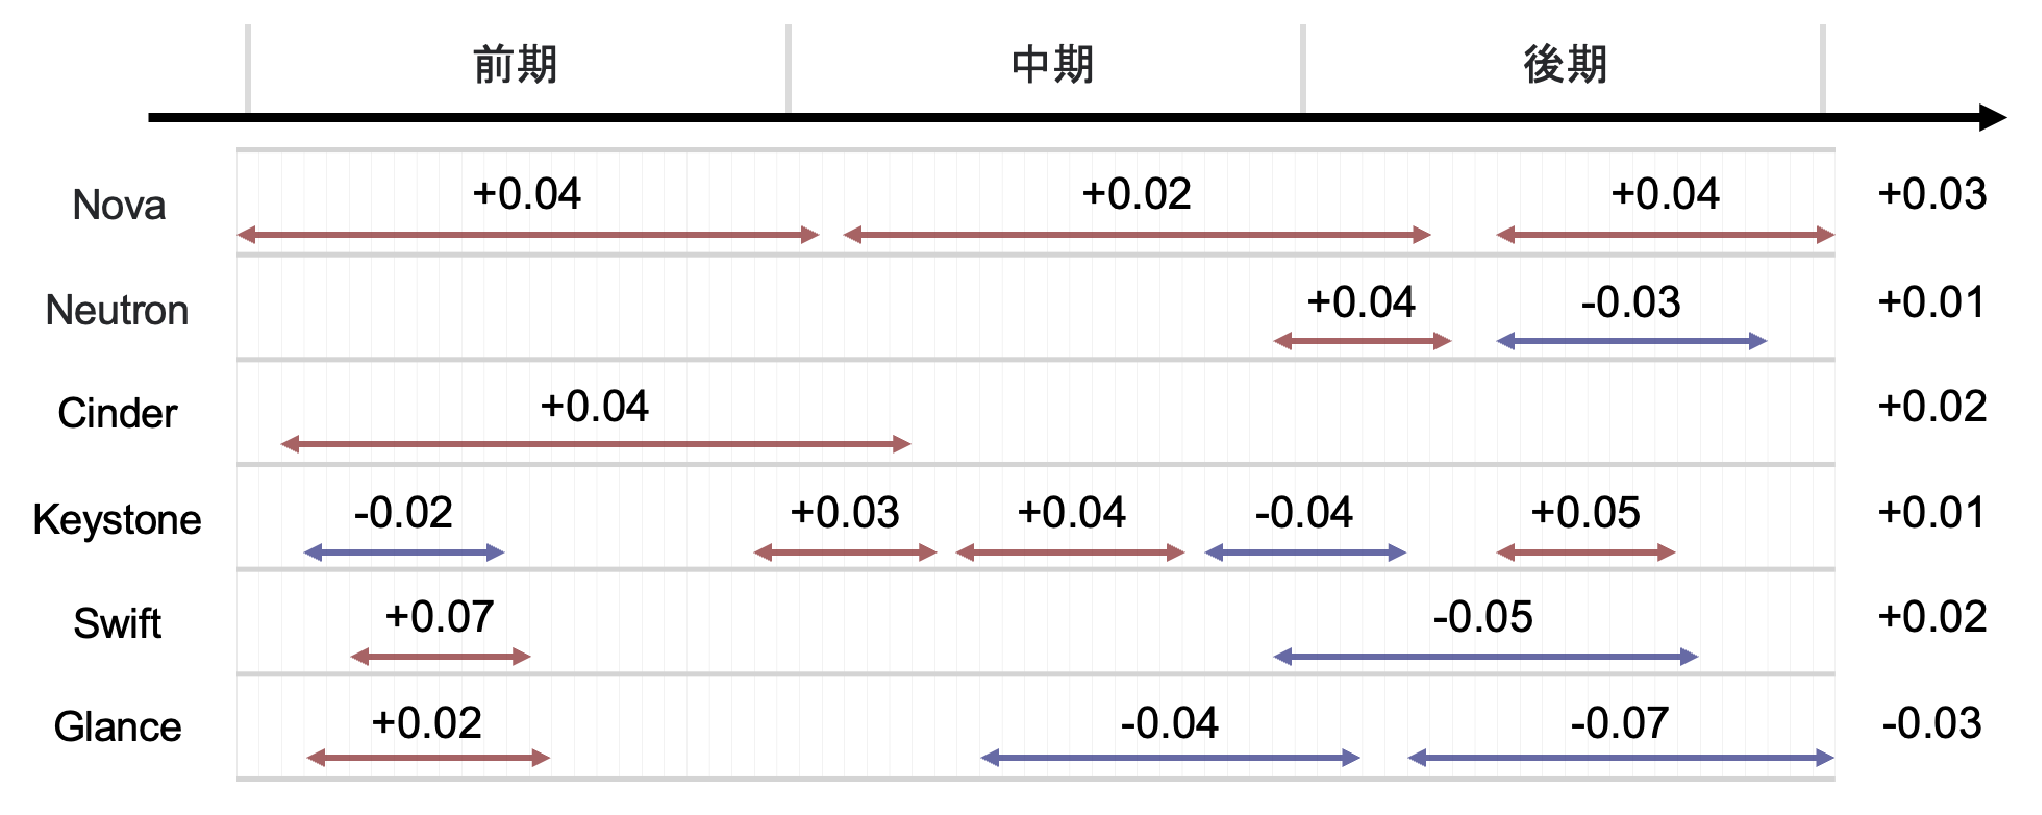
\includegraphics[width=1.0\textwidth]{Uenaka_fig/RQ2_result/review_P.pdf}
    \caption{向上期間,低下期間,リリースまでの全期間における適合率の差の平均値}
    \label{fig:review_prepare_P}
\end{center}
\end{figure}
%-----------------------

%-----------------------
\begin{figure}[t]
\begin{center}
    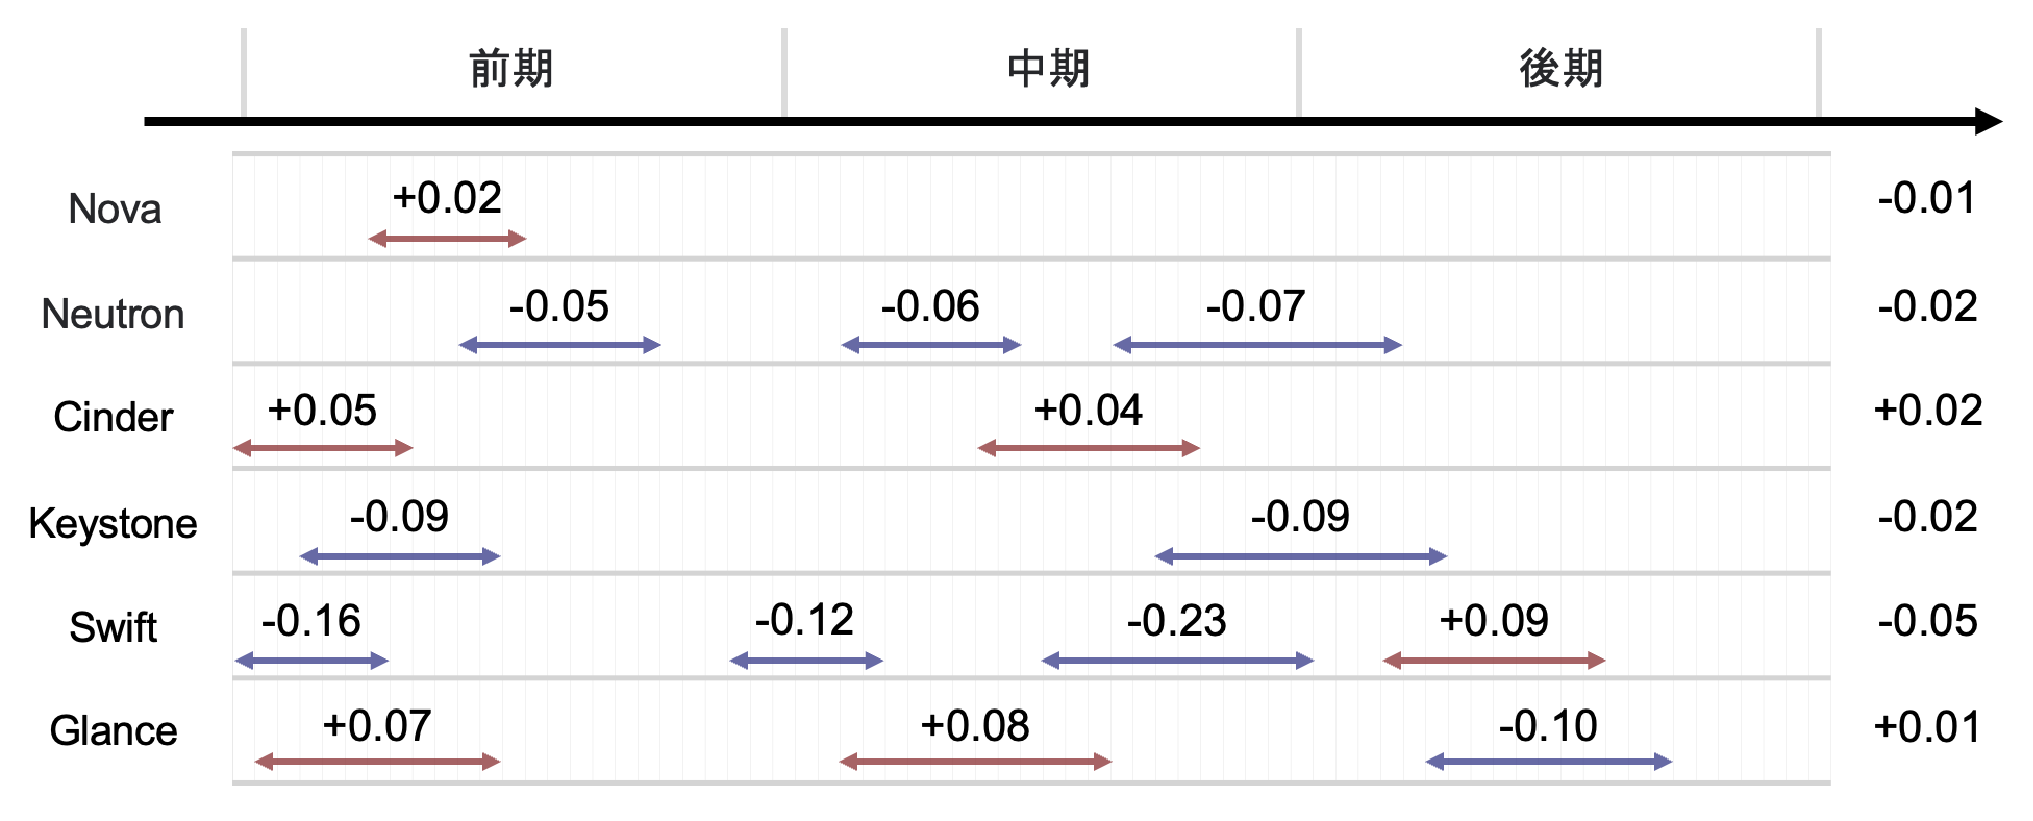
\includegraphics[width=1.0\textwidth]{Uenaka_fig/RQ2_result/review_R.pdf}
    \caption{向上期間,低下期間,リリースまでの全期間における再現率の差の平均値}
    \label{fig:review_prepare_R}
\end{center}
\end{figure}
%-----------------------

%-----------------------
\begin{figure}[t]
\begin{center}
    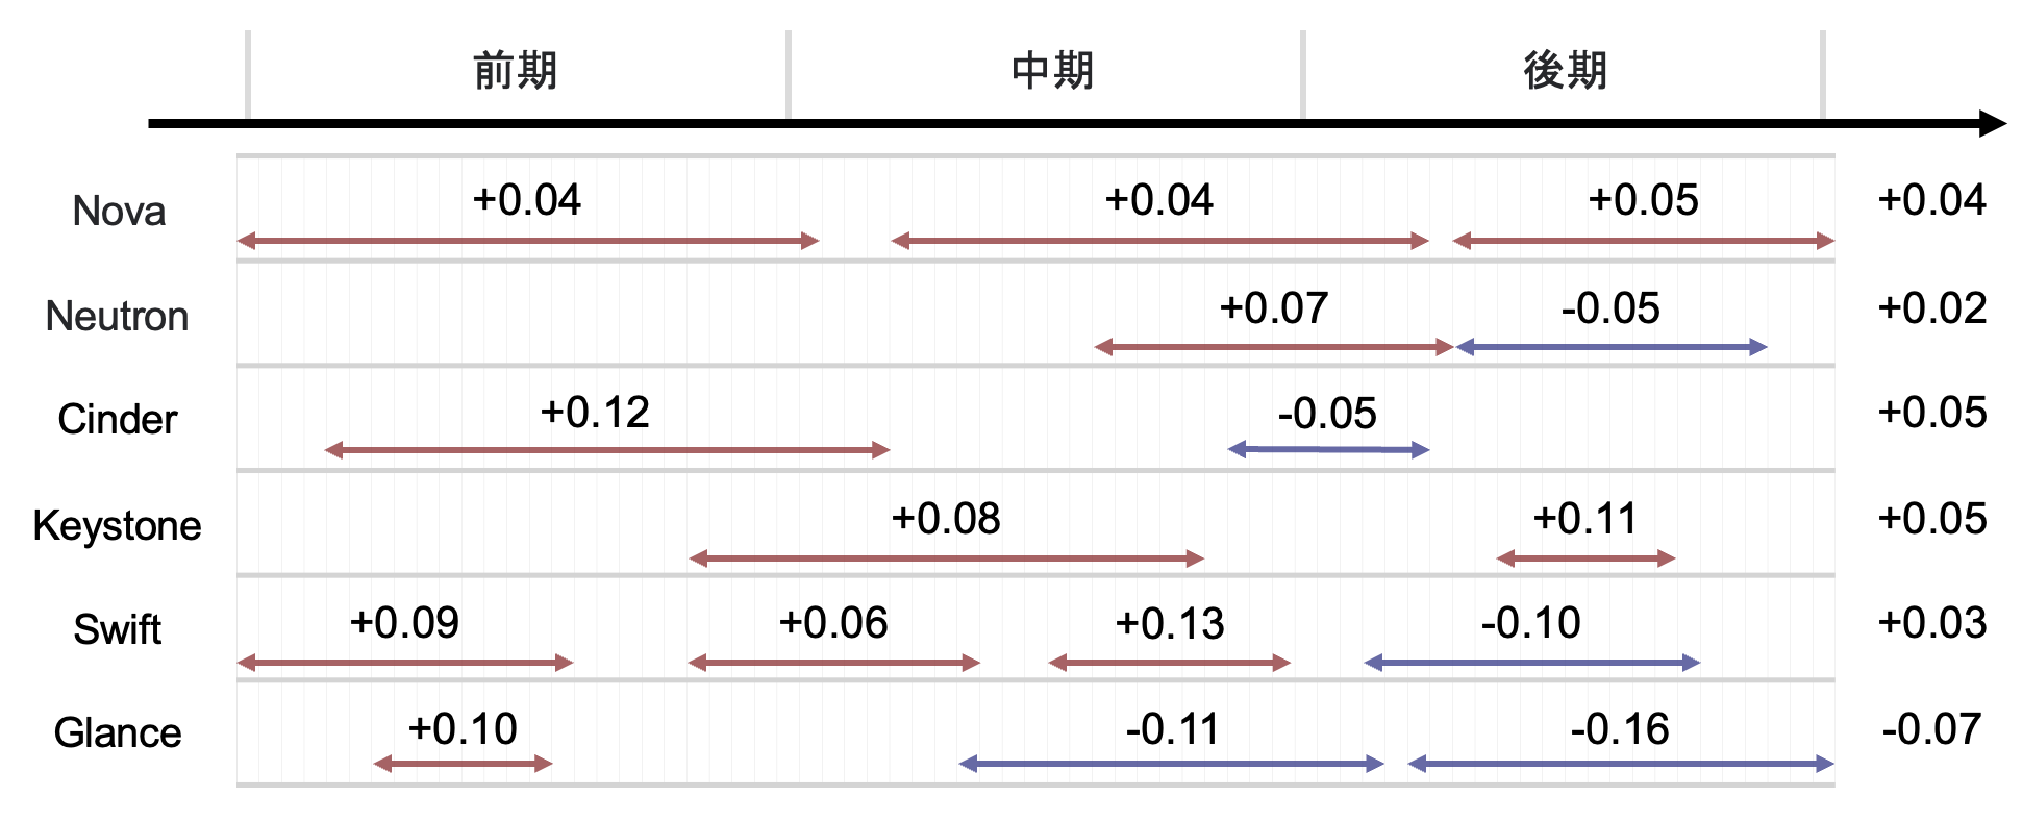
\includegraphics[width=1.0\textwidth]{Uenaka_fig/RQ2_result/review_S.pdf}
    \caption{向上期間,低下期間,リリースまでの全期間における特異度の差の平均値}
    \label{fig:review_prepare_S}
\end{center}
\end{figure}
%-----------------------

%-----------------------
\begin{figure}[t]
\begin{center}
    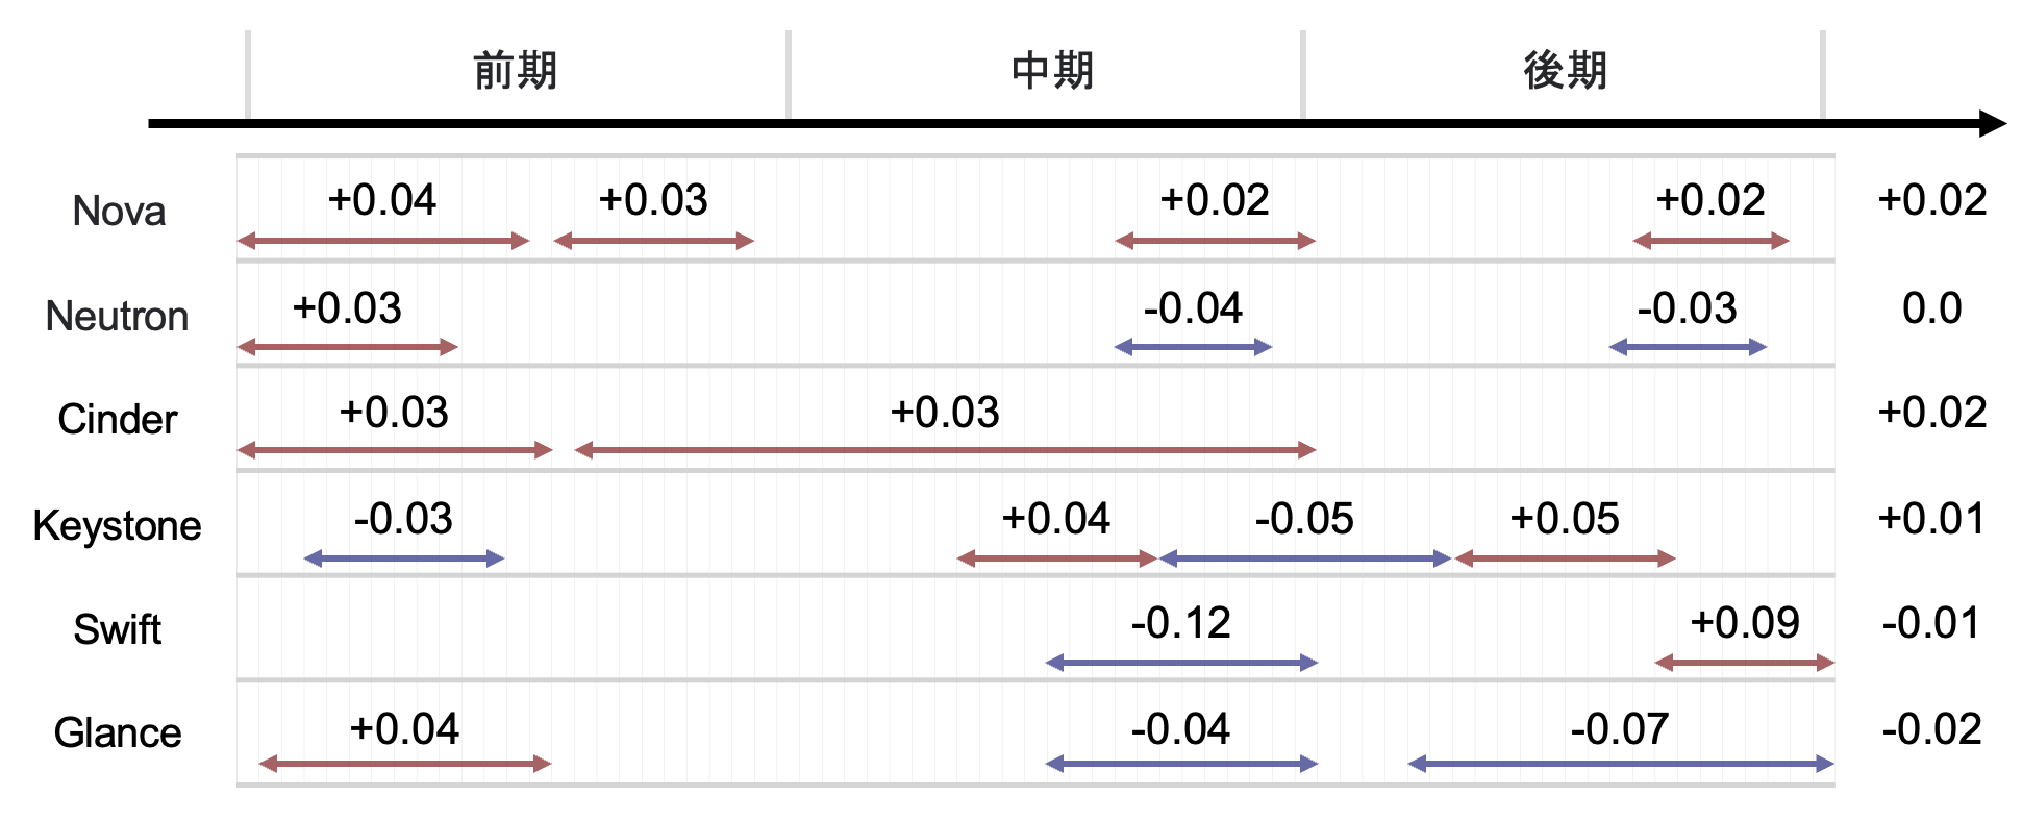
\includegraphics[width=1.0\textwidth]{Uenaka_fig/RQ2_result/review_F.pdf}
    \caption{向上期間,低下期間,リリースまでの全期間におけるF値の差の平均値}
    \label{fig:review_prepare_F}
\end{center}
\end{figure}
%-----------------------


%-----------------------
\clearpage
\begin{figure}[t]
\begin{minipage}{\textwidth}
\vspace{0.08\textheight}
\begin{center}
    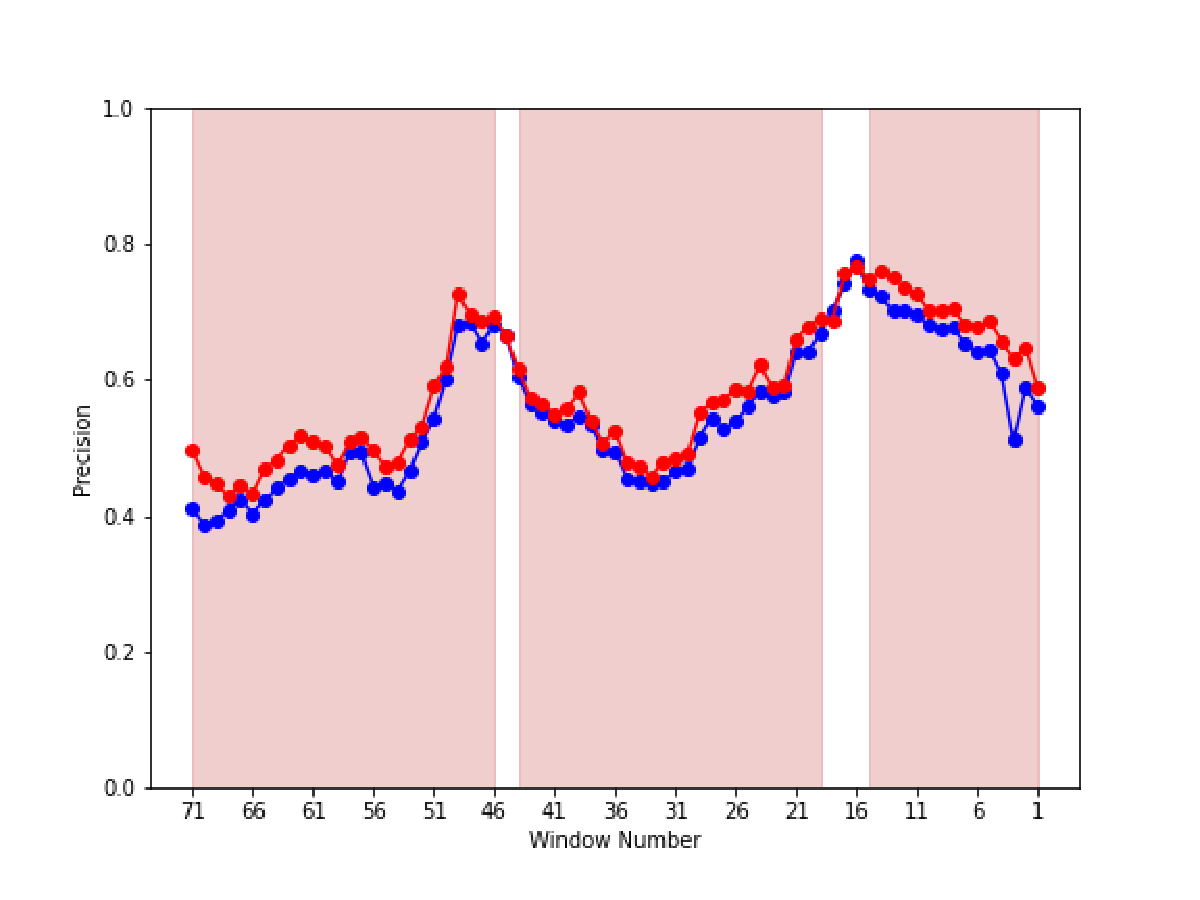
\includegraphics[width=0.495\textwidth]{Uenaka_fig/RQ2_result/Nova/Nova_review_Precision.pdf}
    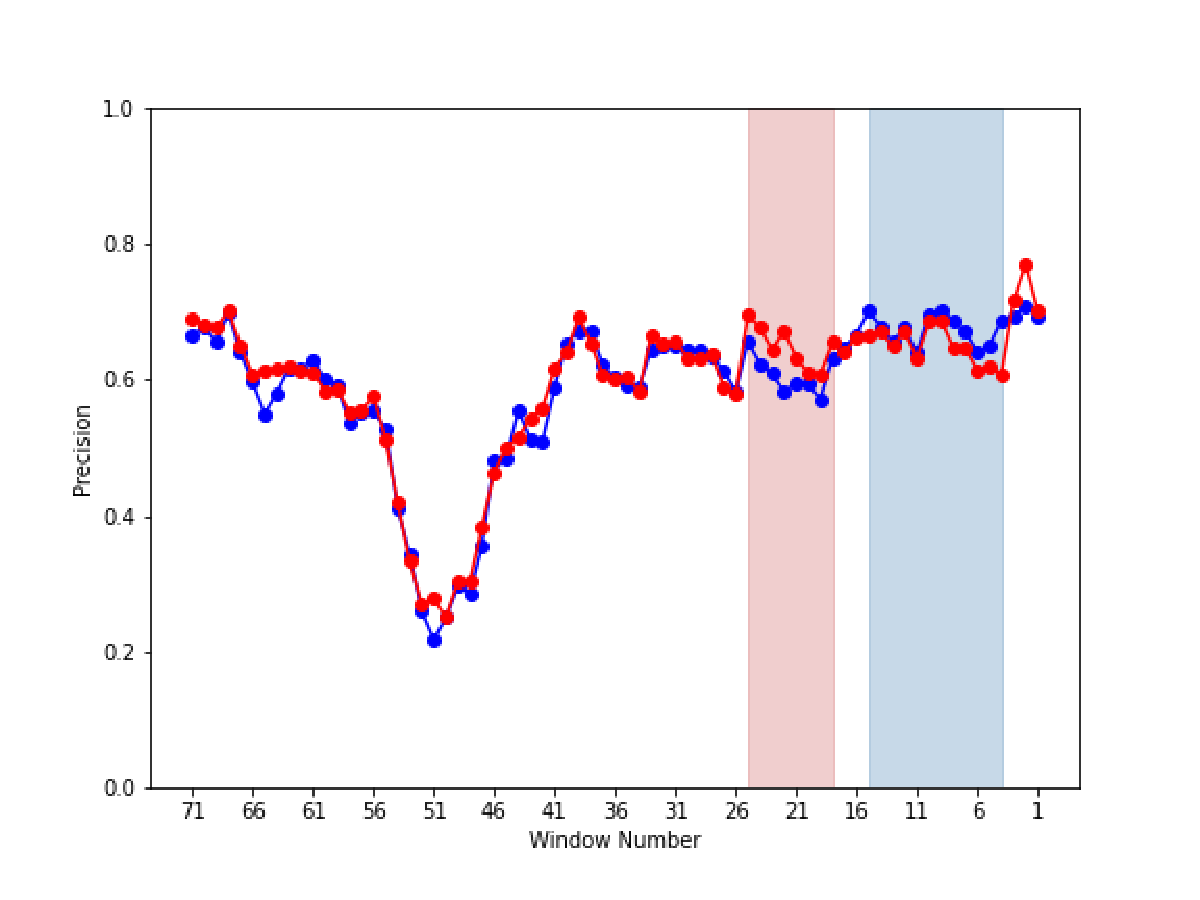
\includegraphics[width=0.495\textwidth]{Uenaka_fig/RQ2_result/Neutron/Neutron_review_Precision.pdf}
    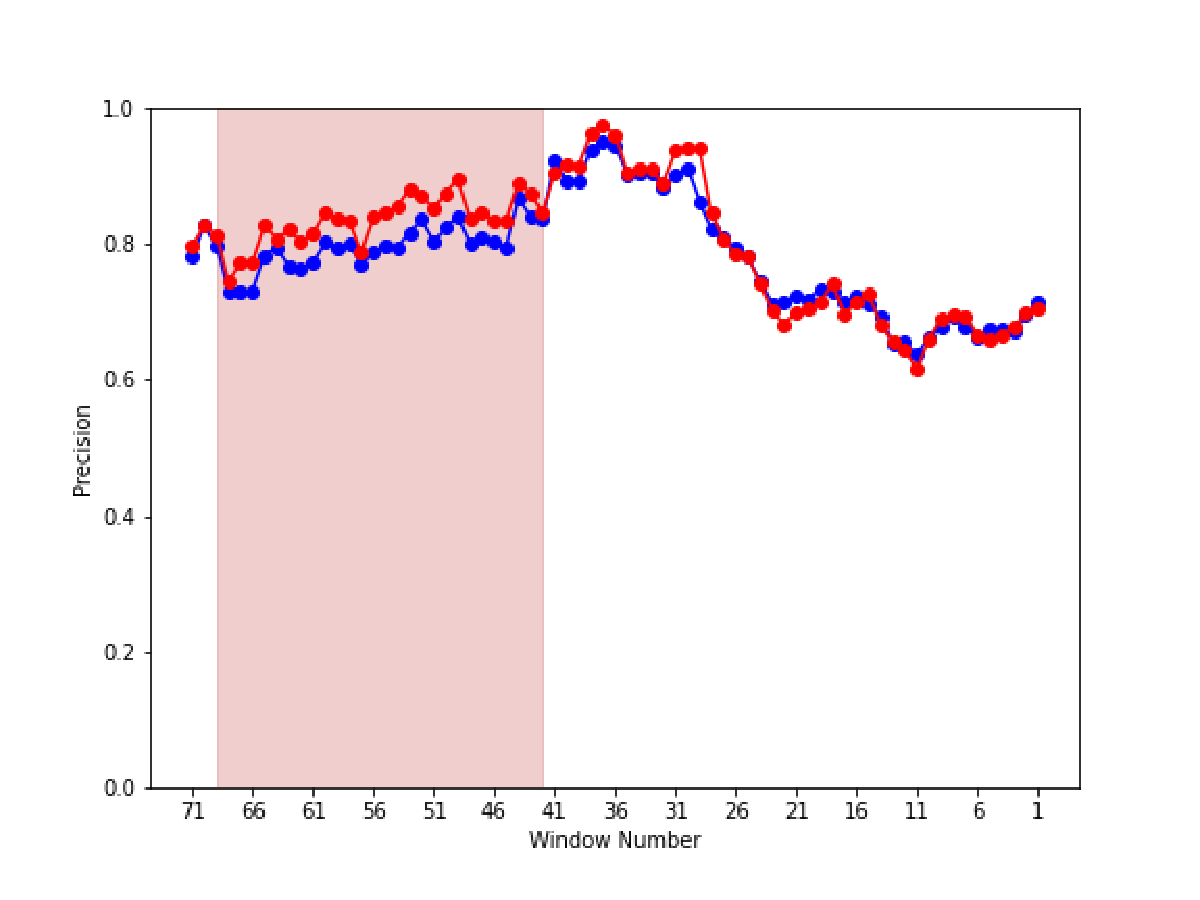
\includegraphics[width=0.495\textwidth]{Uenaka_fig/RQ2_result/Cinder/Cinder_review_Precision.pdf}
    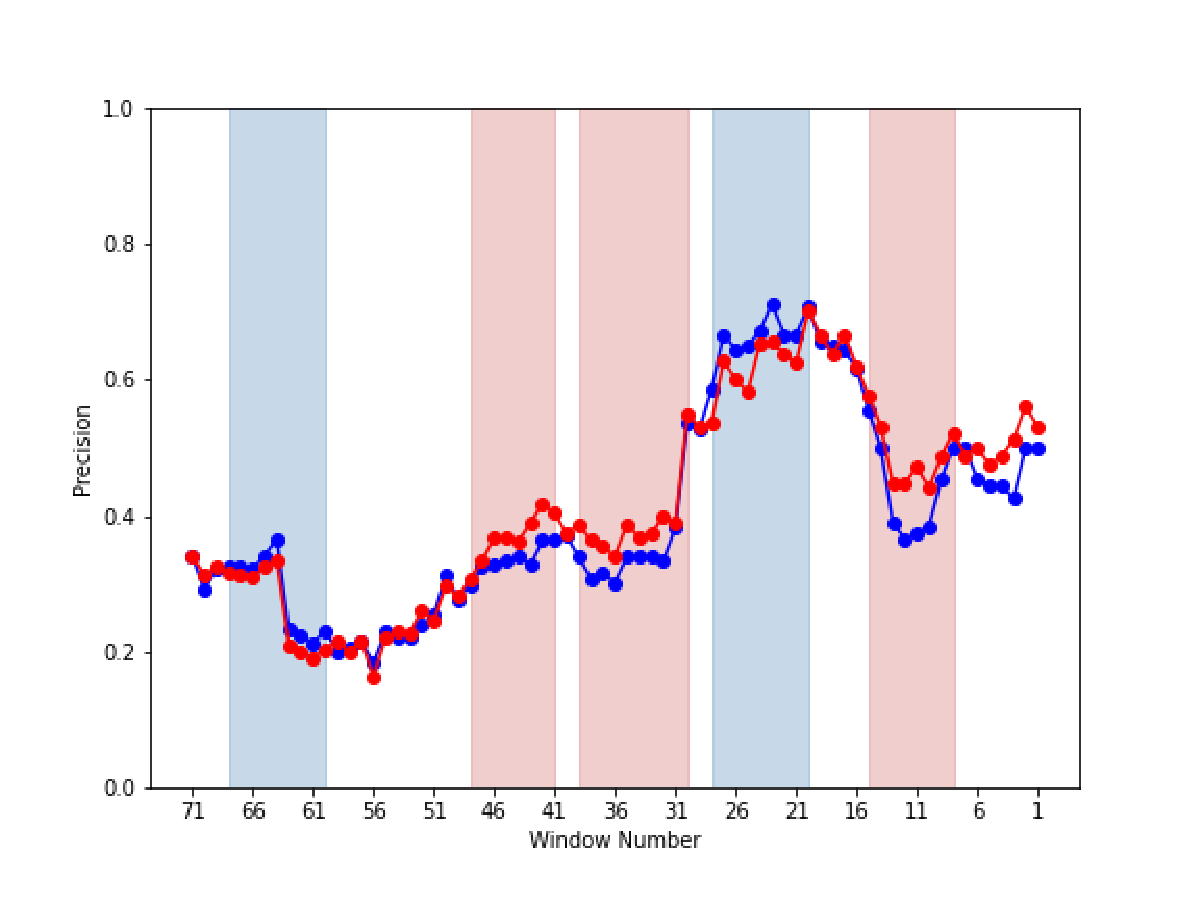
\includegraphics[width=0.495\textwidth]{Uenaka_fig/RQ2_result/Keystone/Keystone_review_Precision.pdf}
    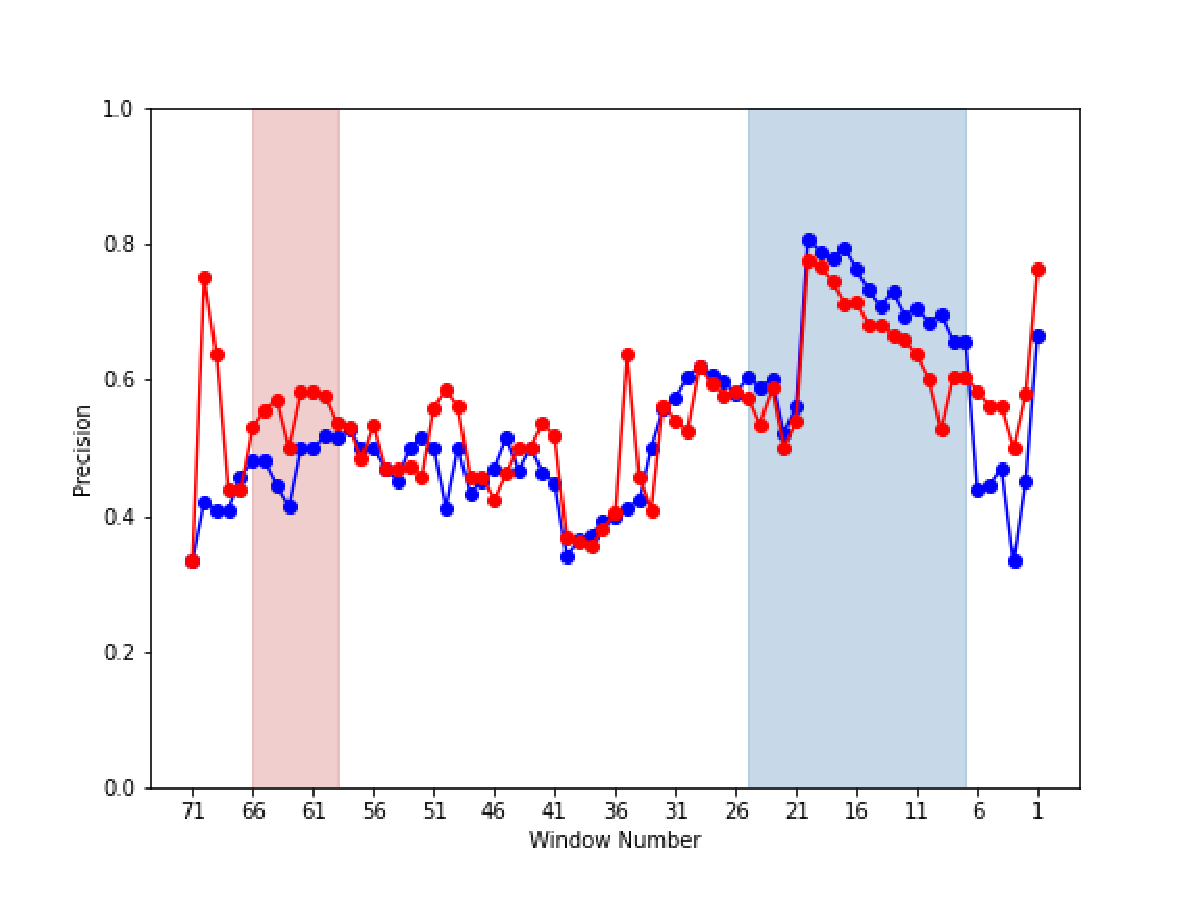
\includegraphics[width=0.495\textwidth]{Uenaka_fig/RQ2_result/Swift/Swift_review_Precision.pdf}
    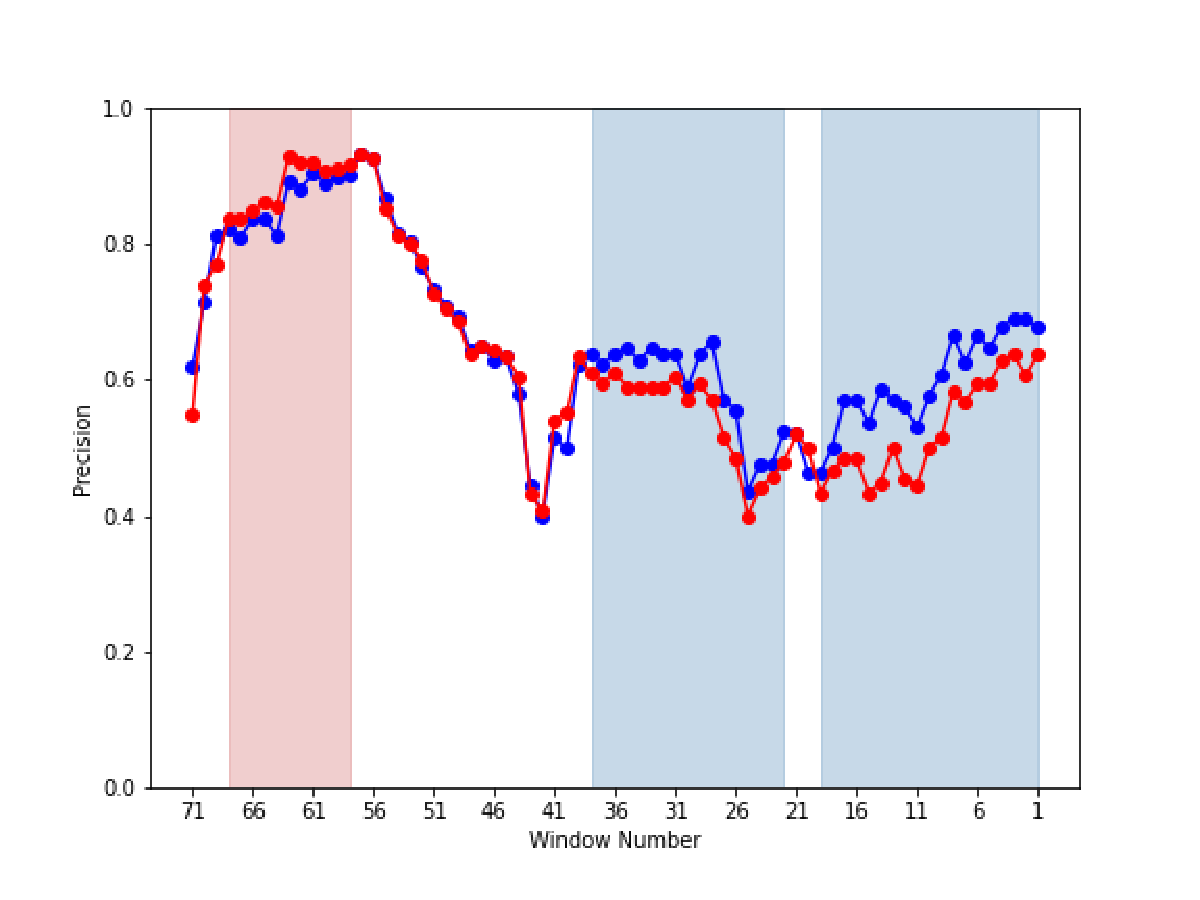
\includegraphics[width=0.495\textwidth]{Uenaka_fig/RQ2_result/Glance/Glance_review_Precision.pdf}
    \caption{レビュー予測モデルの適合率(上段左:Nova,上段右:Neutron,中段左:Cinder,\\ 中段右:Keystone,下段左:Swift,下段右:Glance)(赤:提案モデル,青:ベースラインモデル)}
    \label{fig:review_p}
\end{center}
\vspace{0.08\textheight}
\end{minipage}
\end{figure}
%-----------------------

%-----------------------
\begin{figure}[t]
\begin{minipage}{\textwidth}
\vspace{0.08\textheight}
\begin{center}
    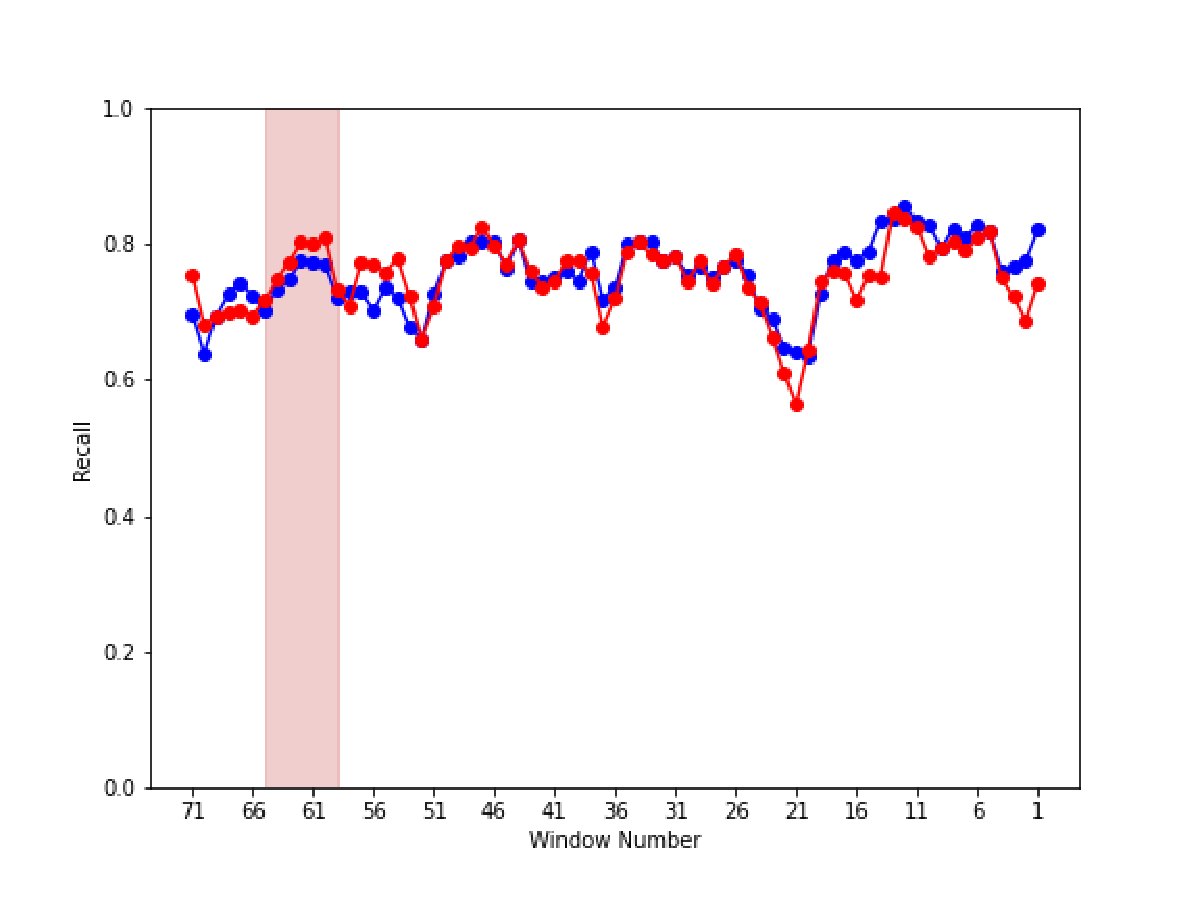
\includegraphics[width=0.495\textwidth]{Uenaka_fig/RQ2_result/Nova/Nova_review_Recall.pdf}
    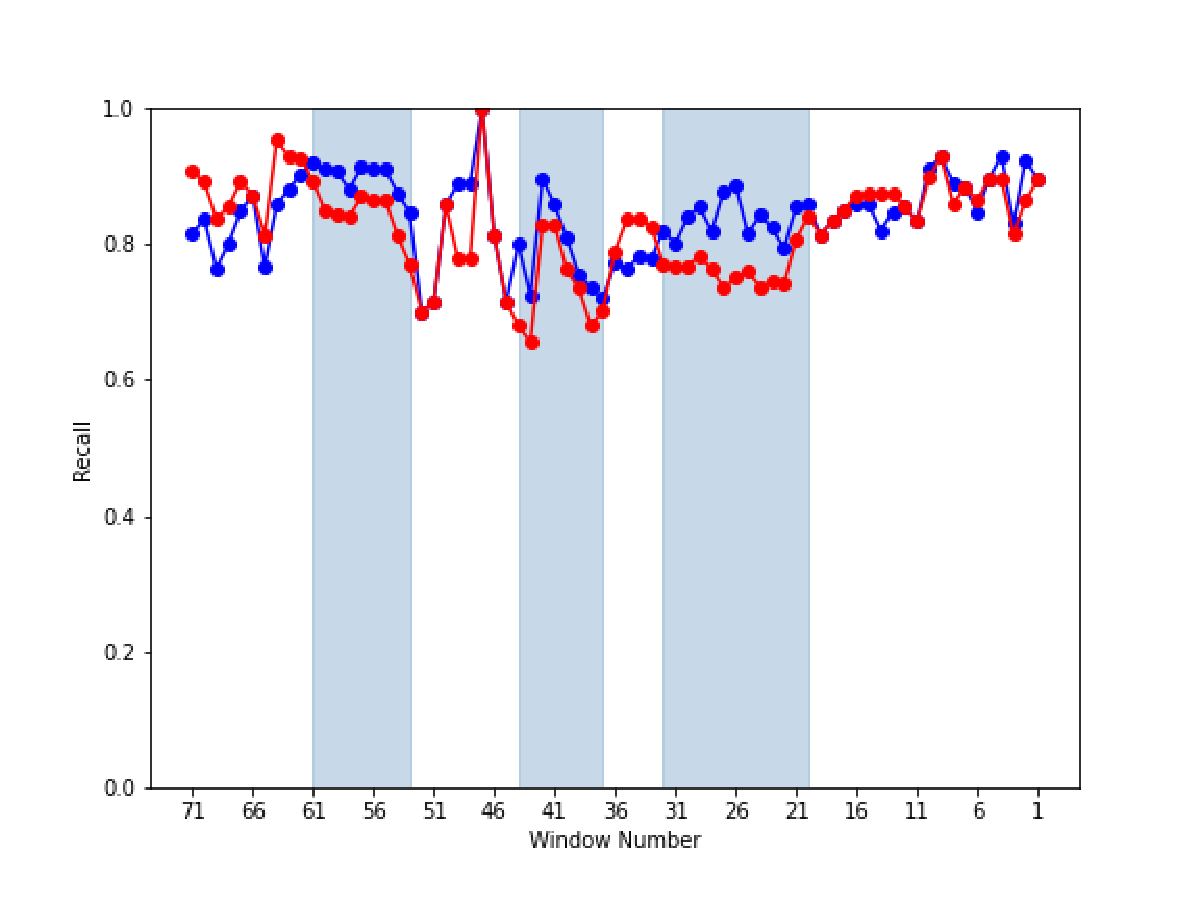
\includegraphics[width=0.495\textwidth]{Uenaka_fig/RQ2_result/Neutron/Neutron_review_Recall.pdf}
    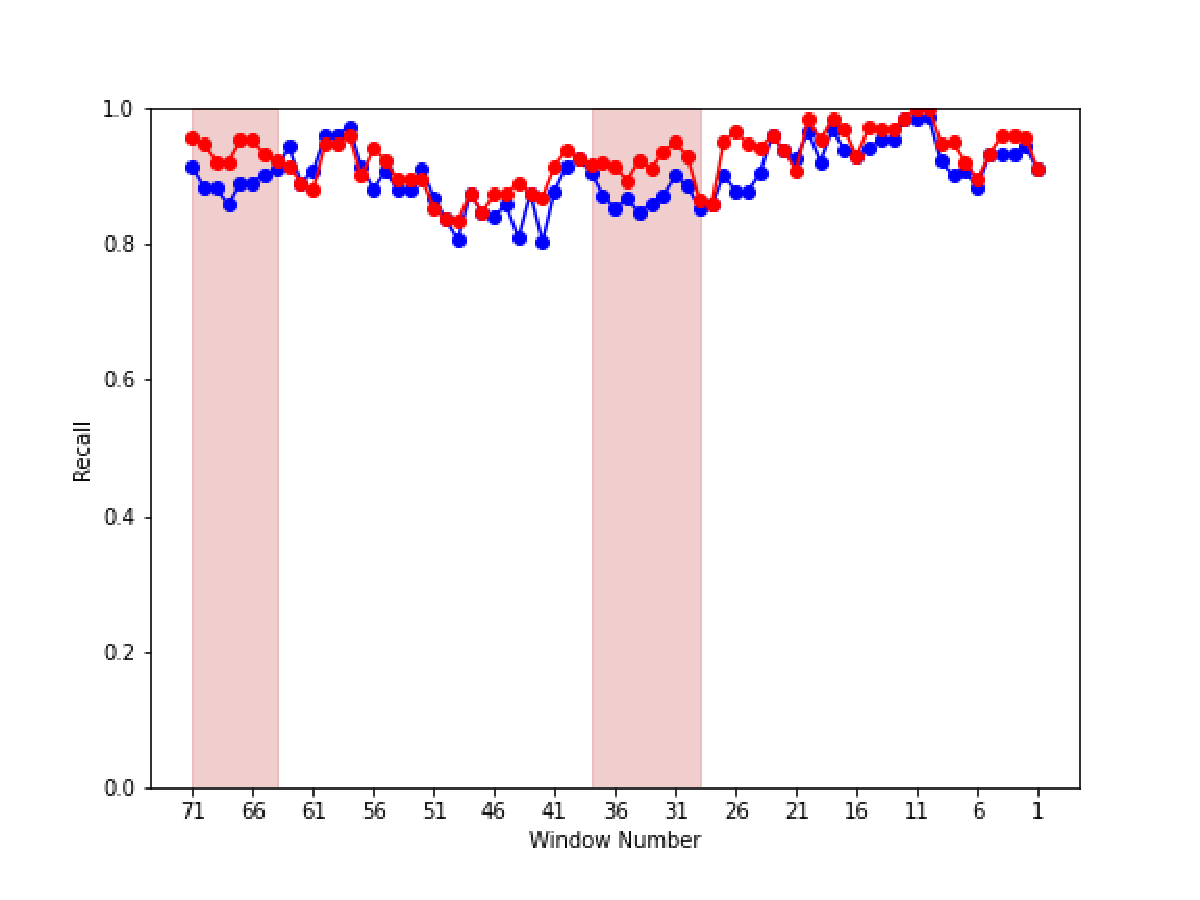
\includegraphics[width=0.495\textwidth]{Uenaka_fig/RQ2_result/Cinder/Cinder_review_Recall.pdf}
    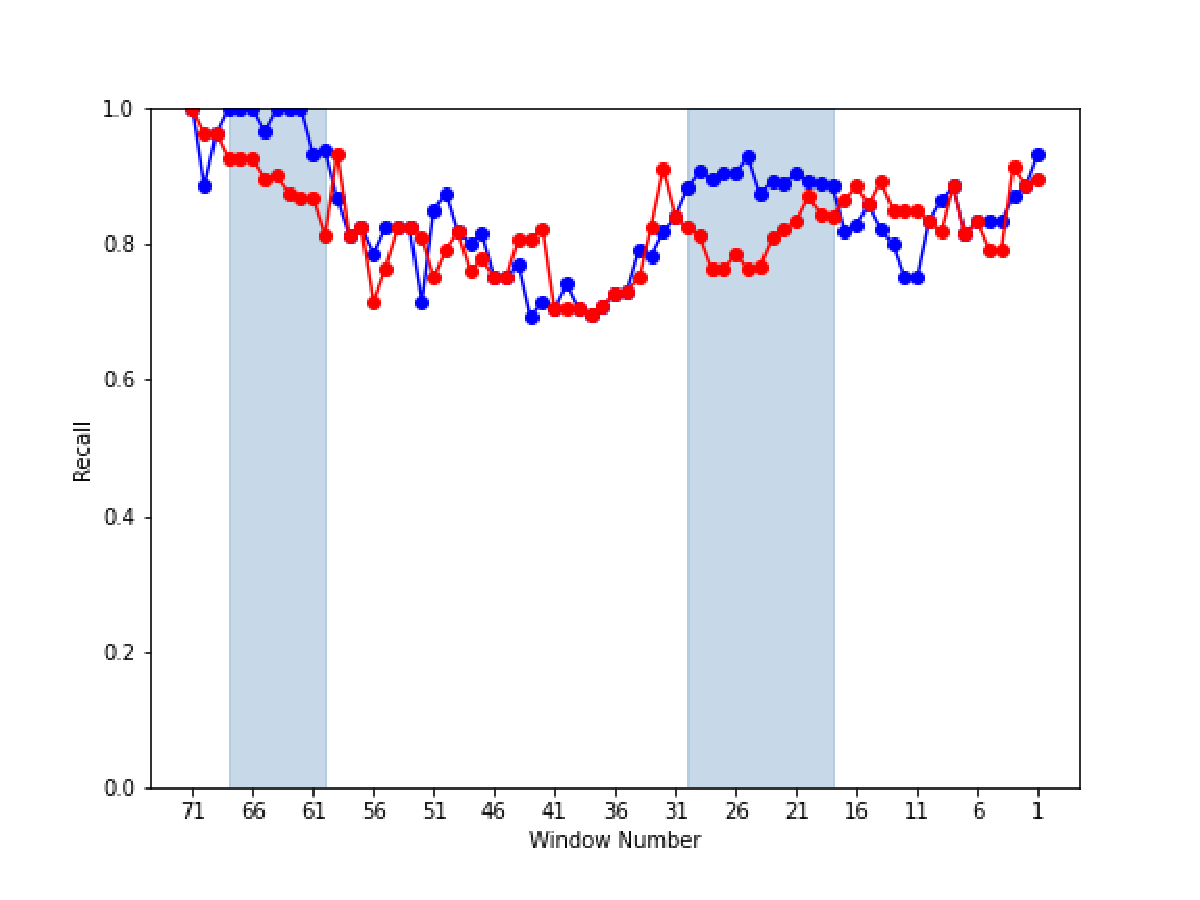
\includegraphics[width=0.495\textwidth]{Uenaka_fig/RQ2_result/Keystone/Keystone_review_Recall.pdf}
    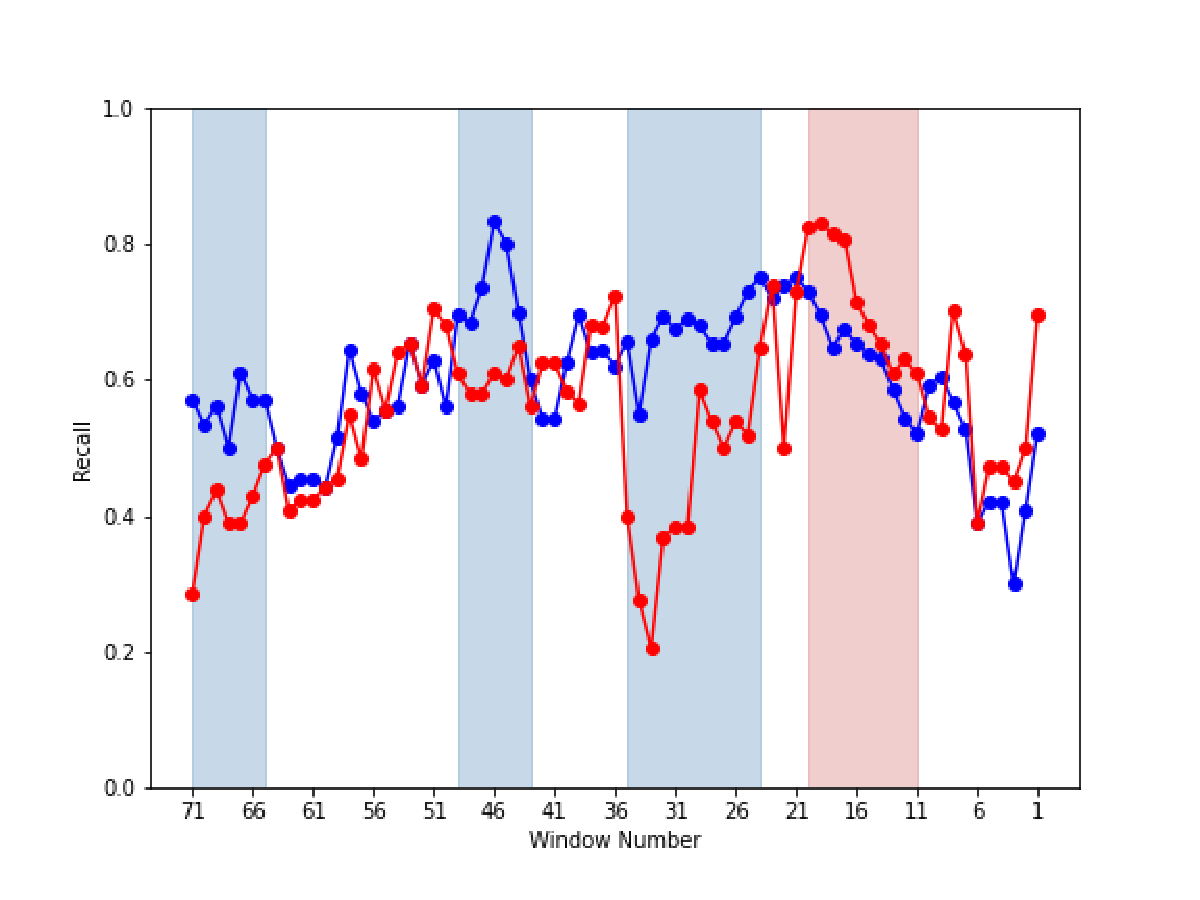
\includegraphics[width=0.495\textwidth]{Uenaka_fig/RQ2_result/Swift/Swift_review_Recall.pdf}
    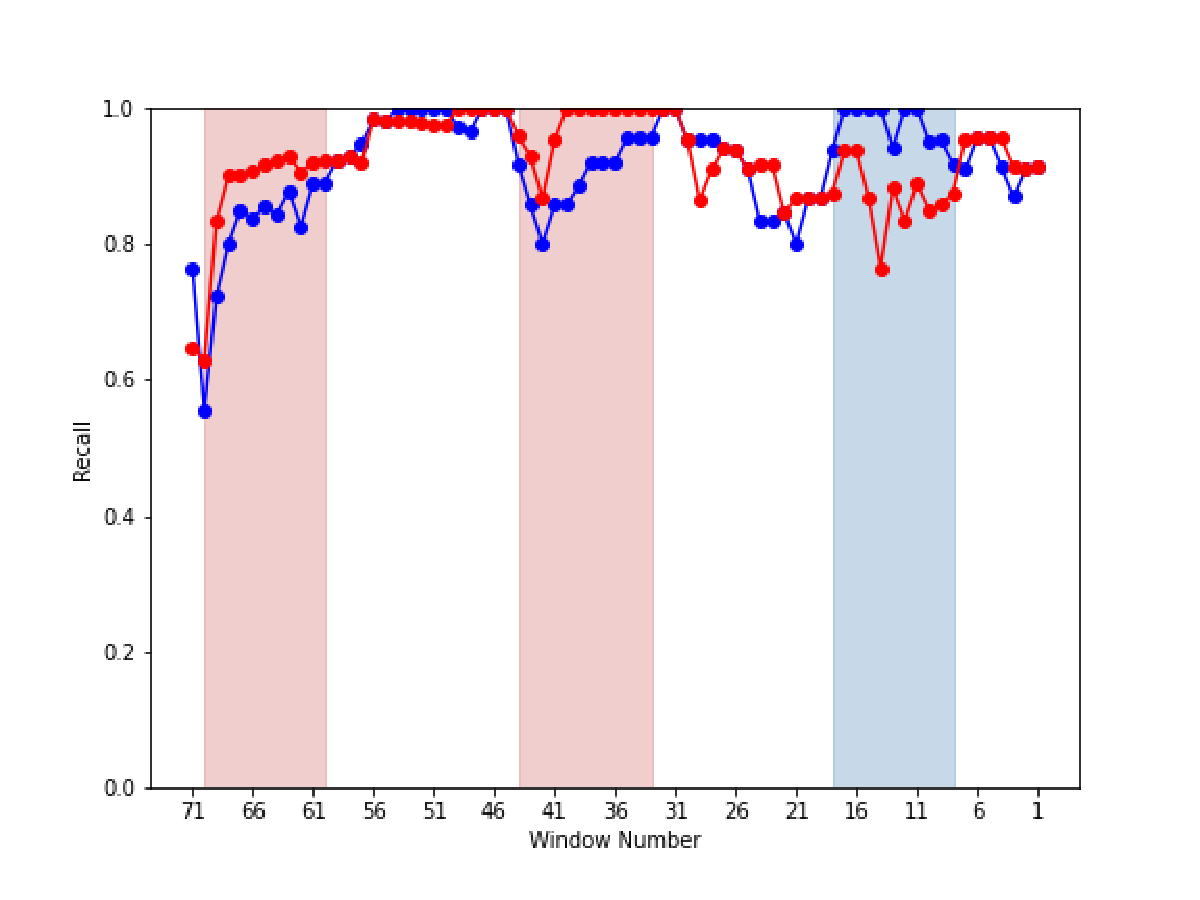
\includegraphics[width=0.495\textwidth]{Uenaka_fig/RQ2_result/Glance/Glance_review_Recall.pdf}
    \caption{レビュー予測モデルの再現率(上段左:Nova,上段右:Neutron,中段左:Cinder,\\ 中段右:Keystone,下段左:Swift,下段右:Glance)(赤:提案モデル,青:ベースラインモデル)}
    \label{fig:review_r}
\end{center}
\vspace{0.08\textheight}
\end{minipage}
\end{figure}
%-----------------------

%-----------------------
\begin{figure}[t]
\begin{minipage}{\textwidth}
\vspace{0.08\textheight}
\begin{center}
    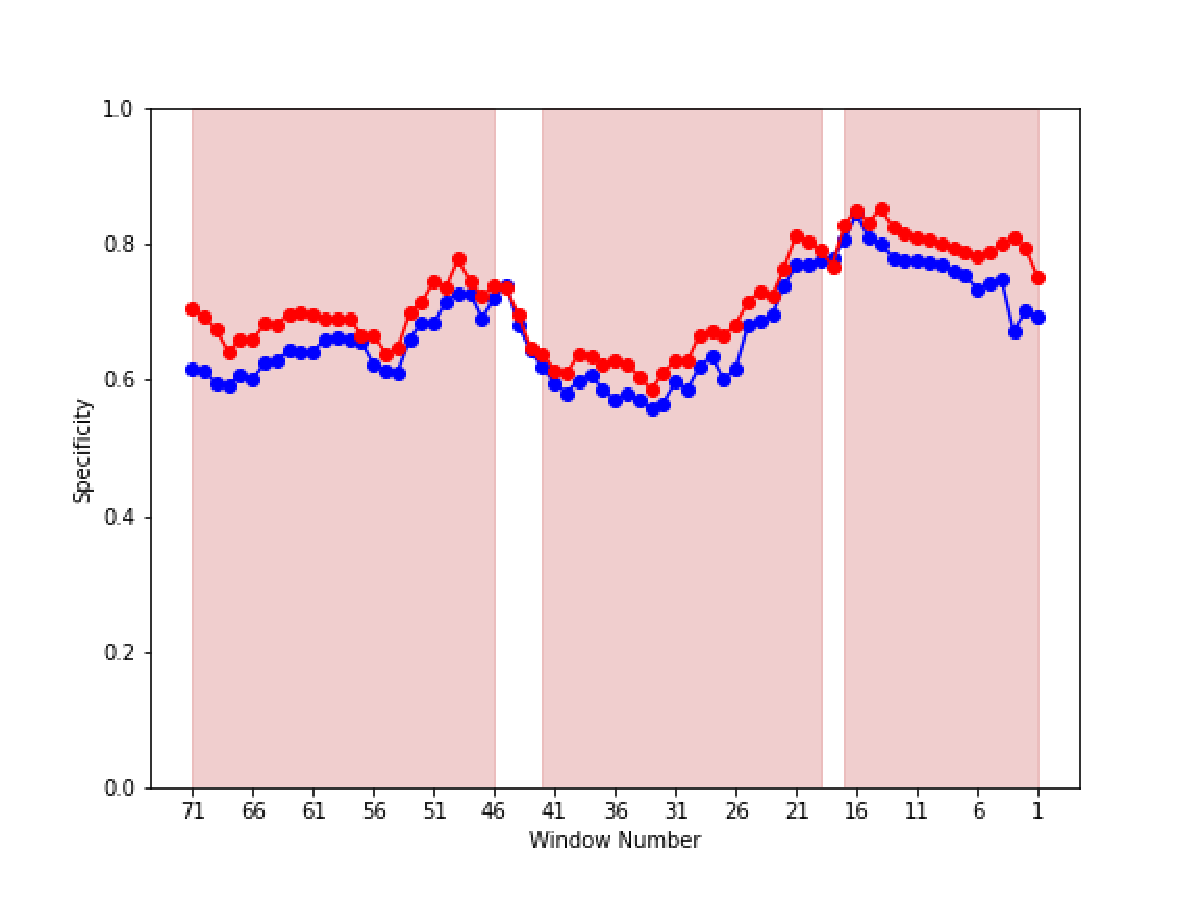
\includegraphics[width=0.495\textwidth]{Uenaka_fig/RQ2_result/Nova/Nova_review_Specificity.pdf}
    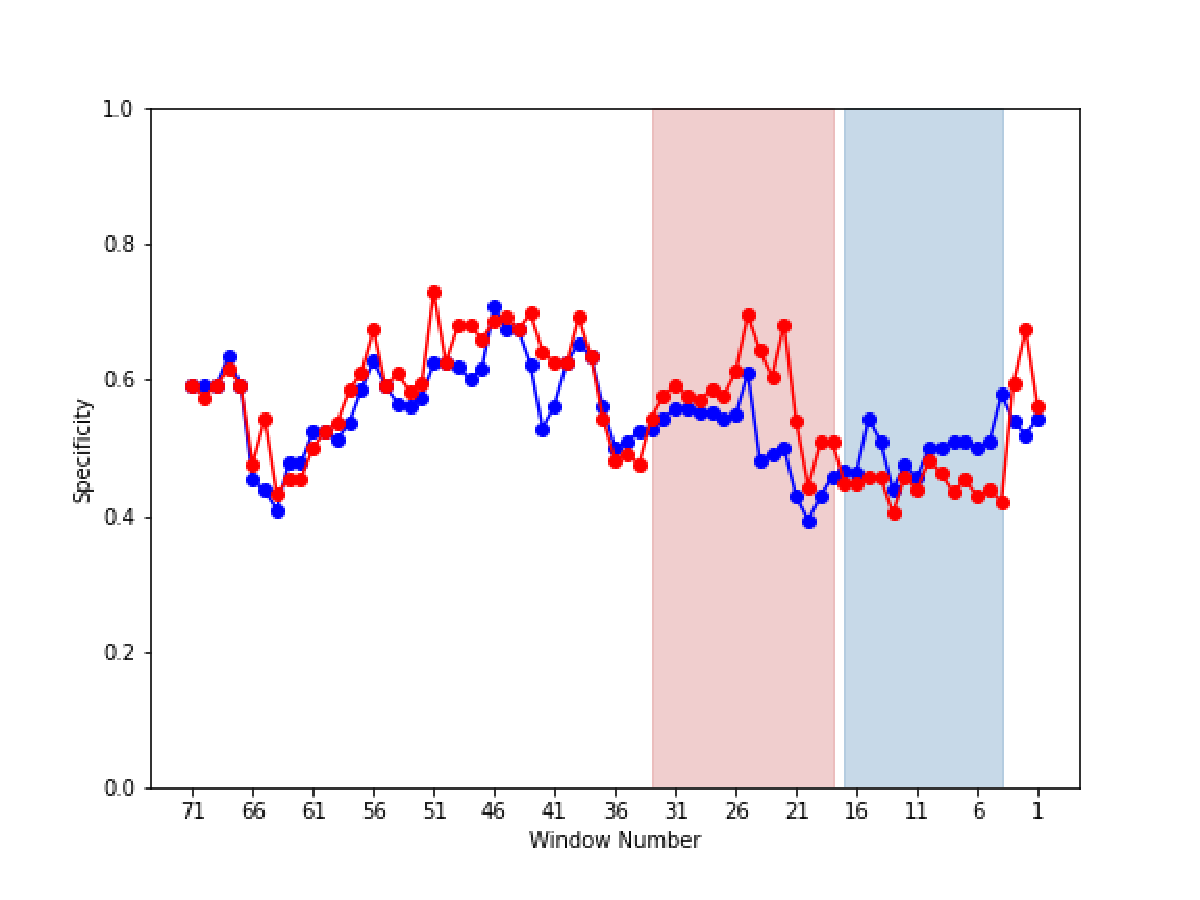
\includegraphics[width=0.495\textwidth]{Uenaka_fig/RQ2_result/Neutron/Neutron_review_Specificity.pdf}
    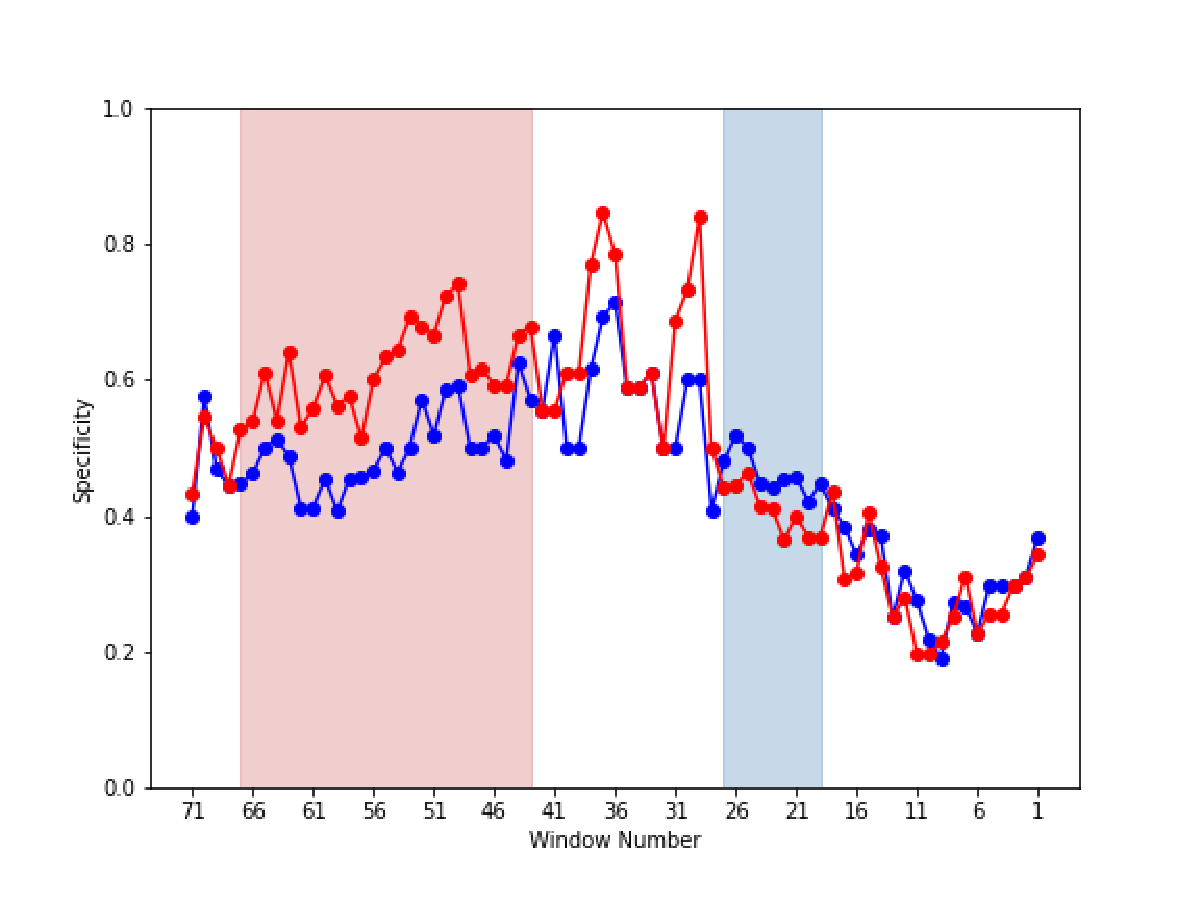
\includegraphics[width=0.495\textwidth]{Uenaka_fig/RQ2_result/Cinder/Cinder_review_Specificity.pdf}
    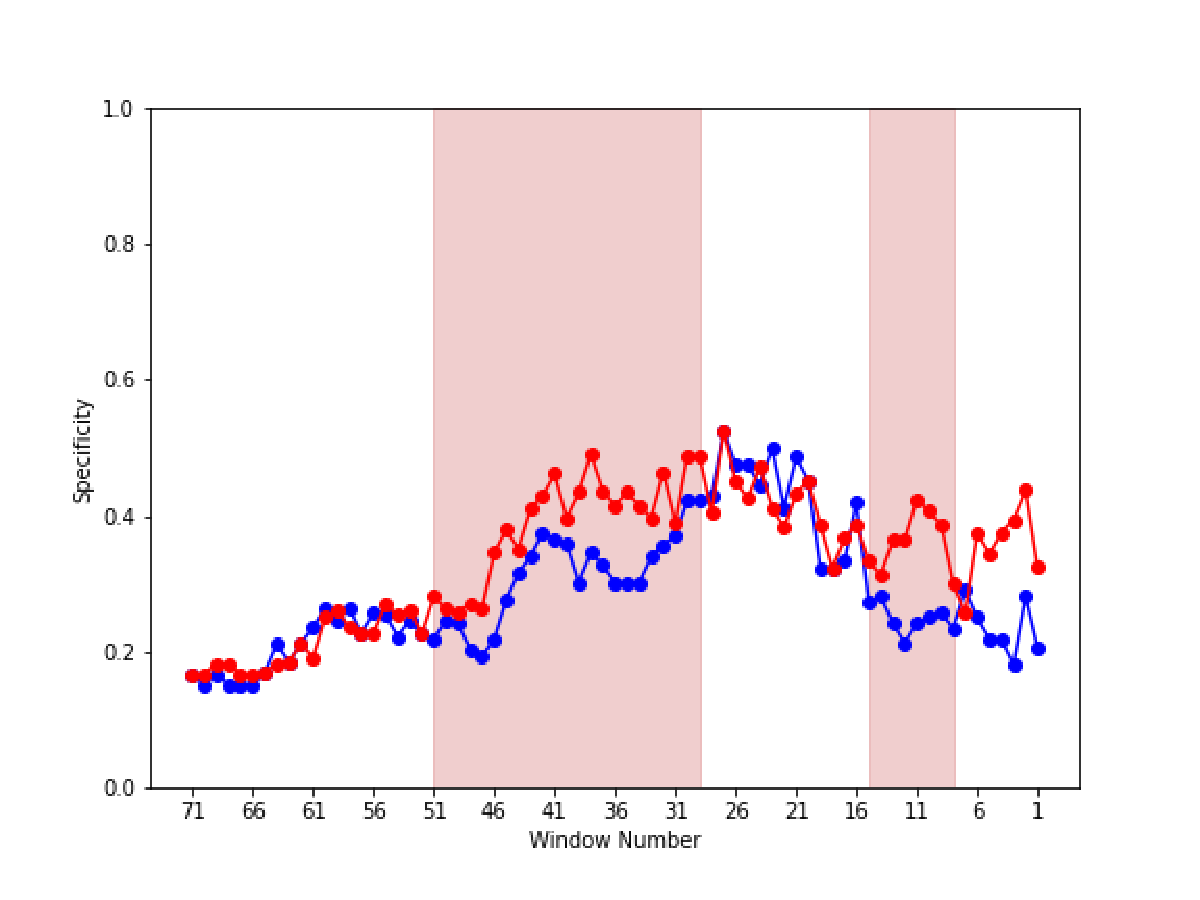
\includegraphics[width=0.495\textwidth]{Uenaka_fig/RQ2_result/Keystone/Keystone_review_Specificity.pdf}
    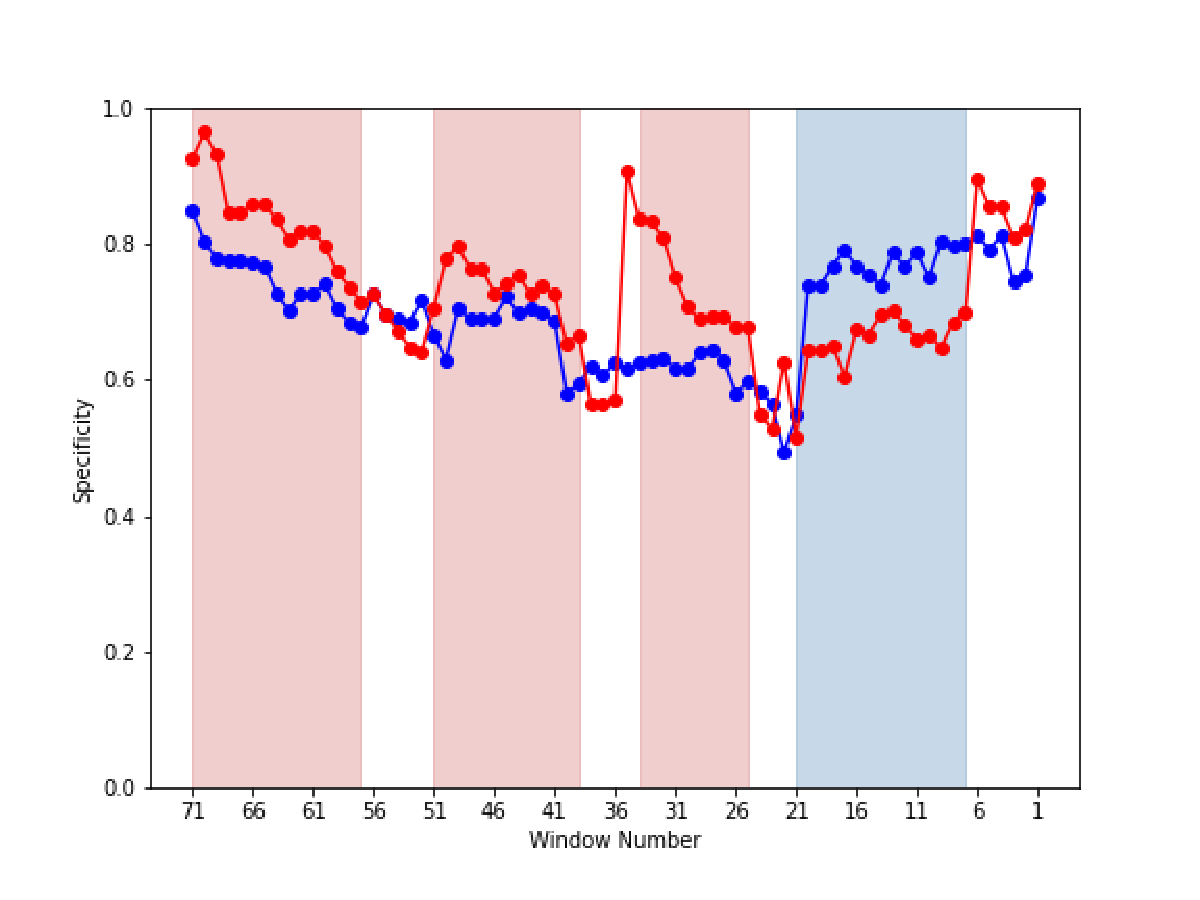
\includegraphics[width=0.495\textwidth]{Uenaka_fig/RQ2_result/Swift/Swift_review_Specificity.pdf}
    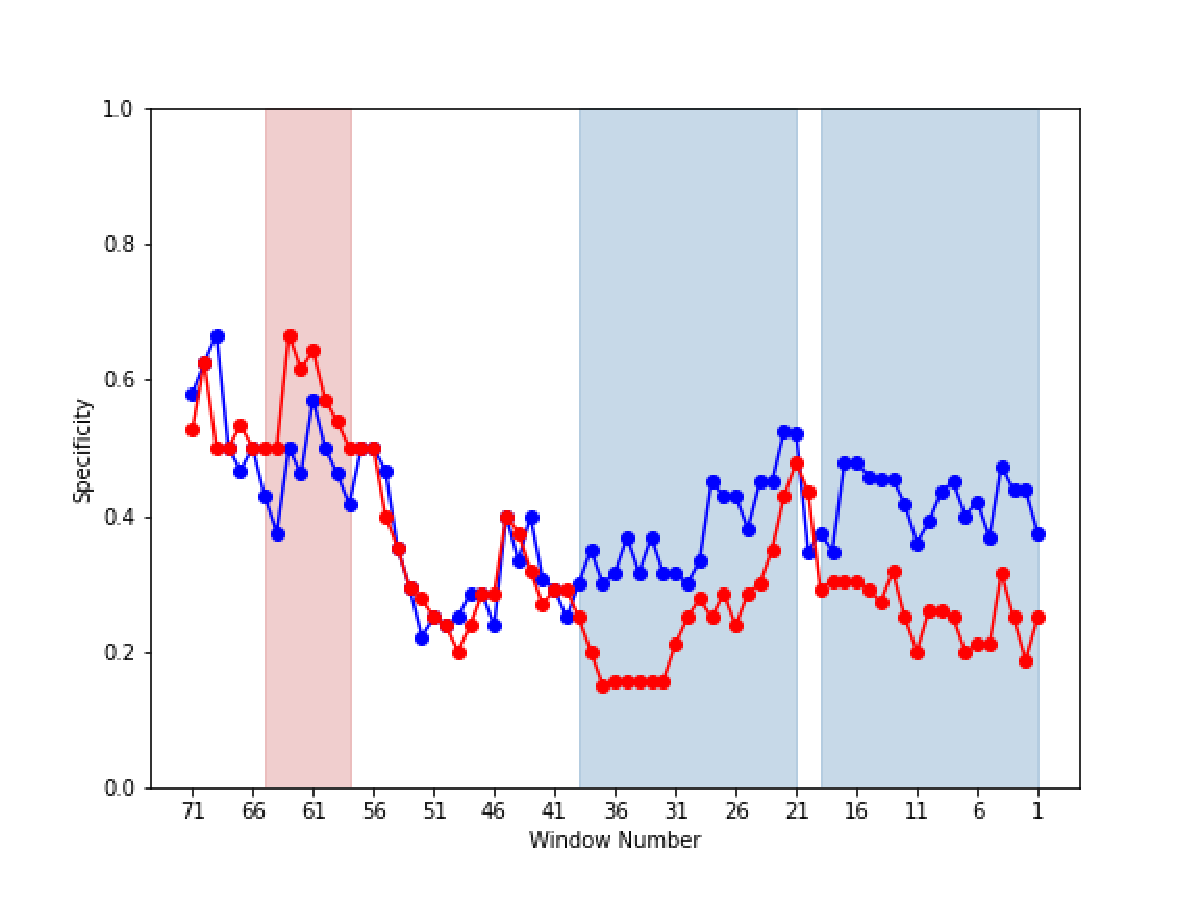
\includegraphics[width=0.495\textwidth]{Uenaka_fig/RQ2_result/Glance/Glance_review_Specificity.pdf}
    \caption{レビュー予測モデルの特異度(上段左:Nova,上段右:Neutron,中段左:Cinder,\\ 中段右:Keystone,下段左:Swift,下段右:Glance)(赤:提案モデル,青:ベースラインモデル)}
    \label{fig:review_spec}
\end{center}
\vspace{0.08\textheight}
\end{minipage}
\end{figure}
%-----------------------

%-----------------------
\begin{figure}[t]
\begin{center}
    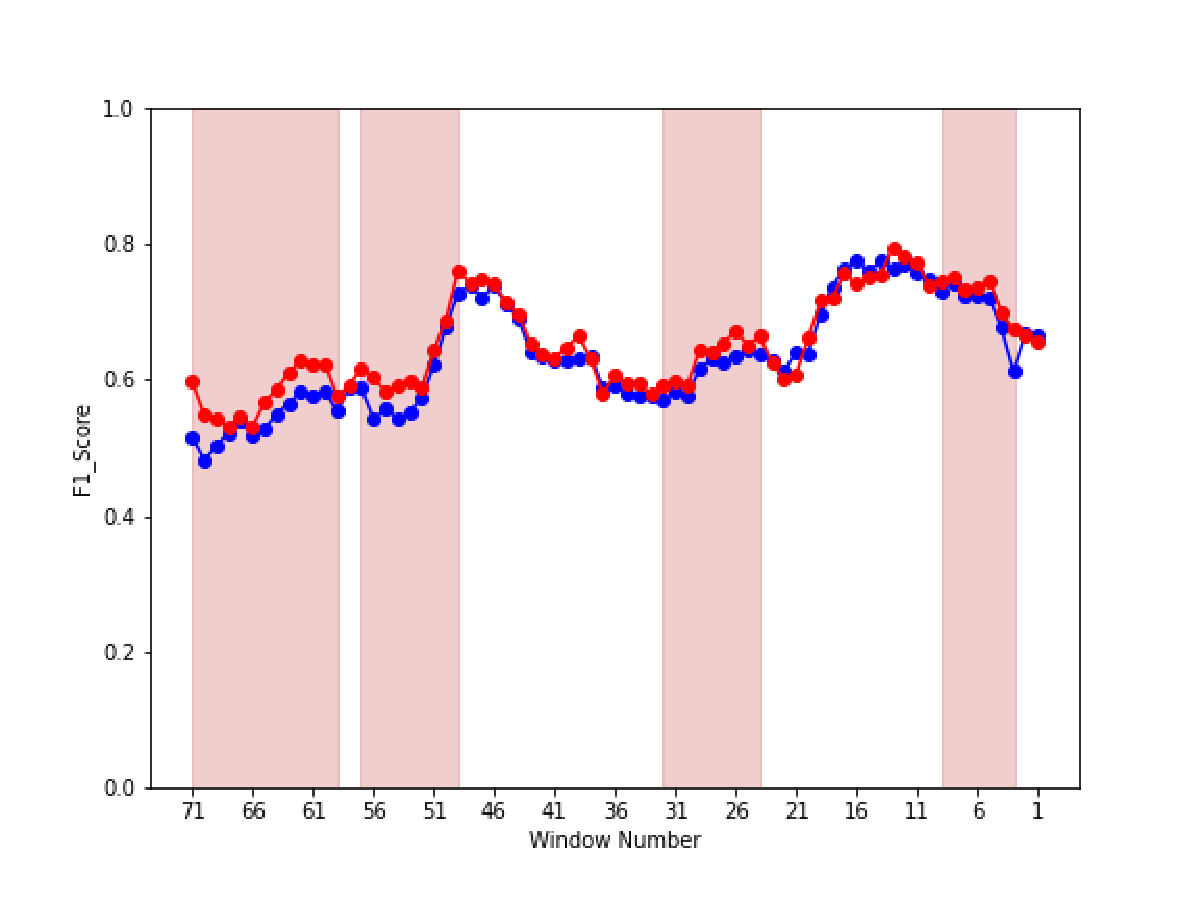
\includegraphics[width=0.495\textwidth]{Uenaka_fig/RQ2_result/Nova/Nova_review_F1.pdf}
    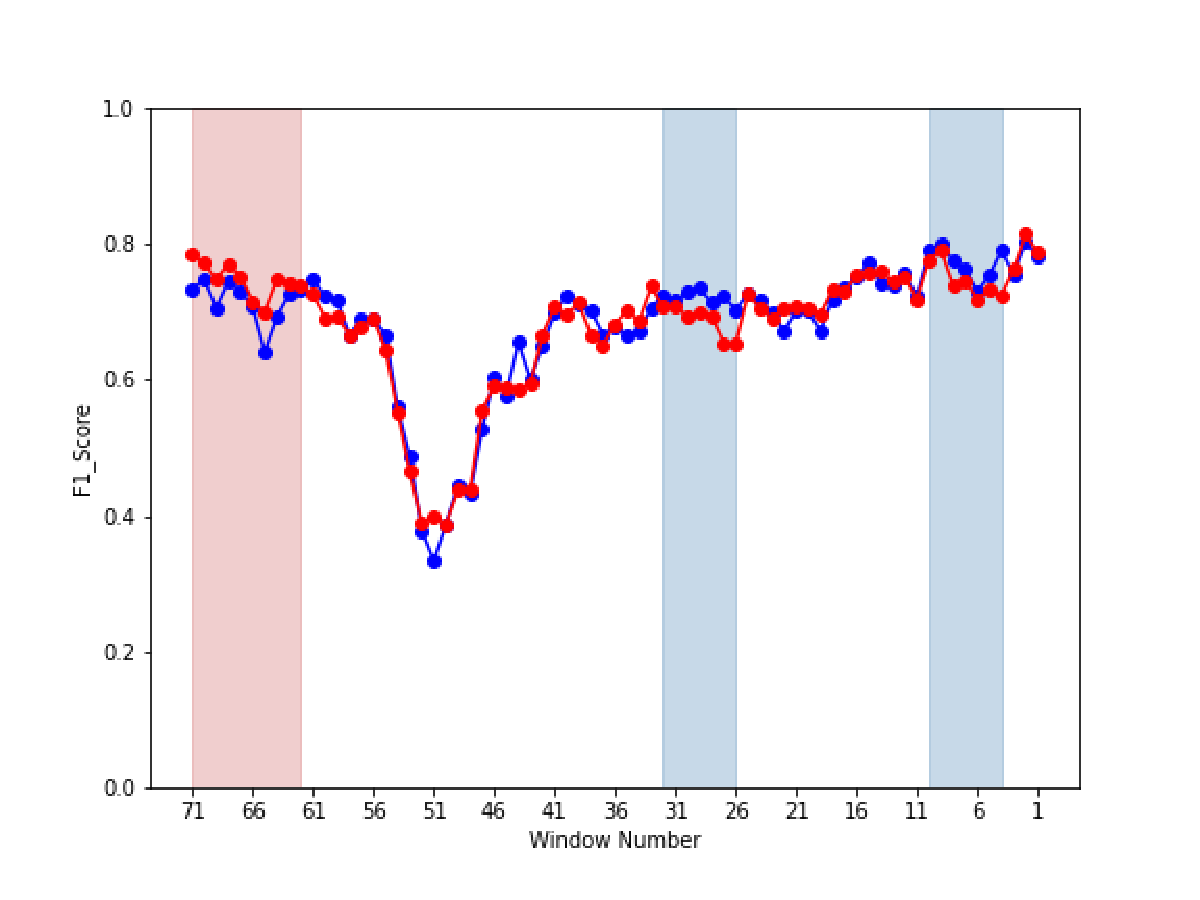
\includegraphics[width=0.495\textwidth]{Uenaka_fig/RQ2_result/Neutron/Neutron_review_F1.pdf}
    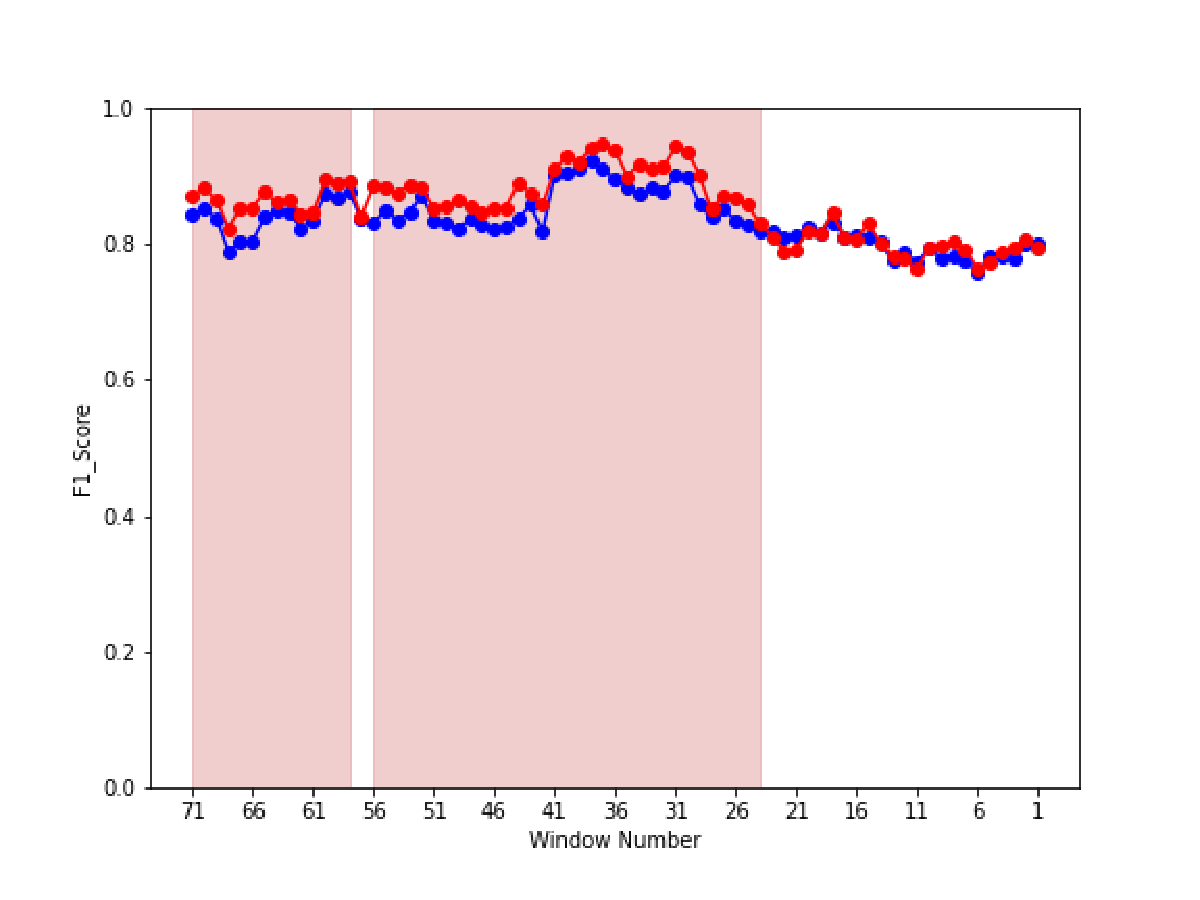
\includegraphics[width=0.495\textwidth]{Uenaka_fig/RQ2_result/Cinder/Cinder_review_F1.pdf}
    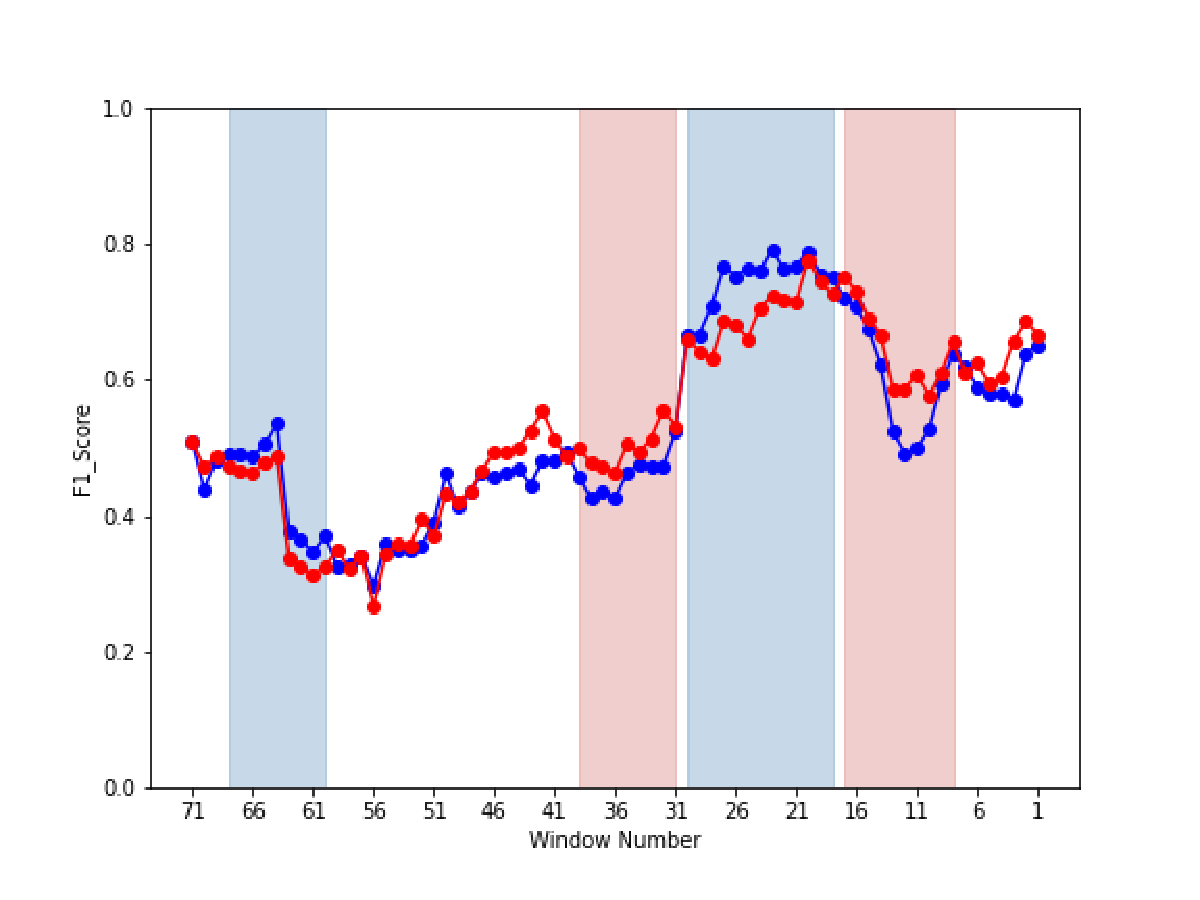
\includegraphics[width=0.495\textwidth]{Uenaka_fig/RQ2_result/Keystone/Keystone_review_F1.pdf}
    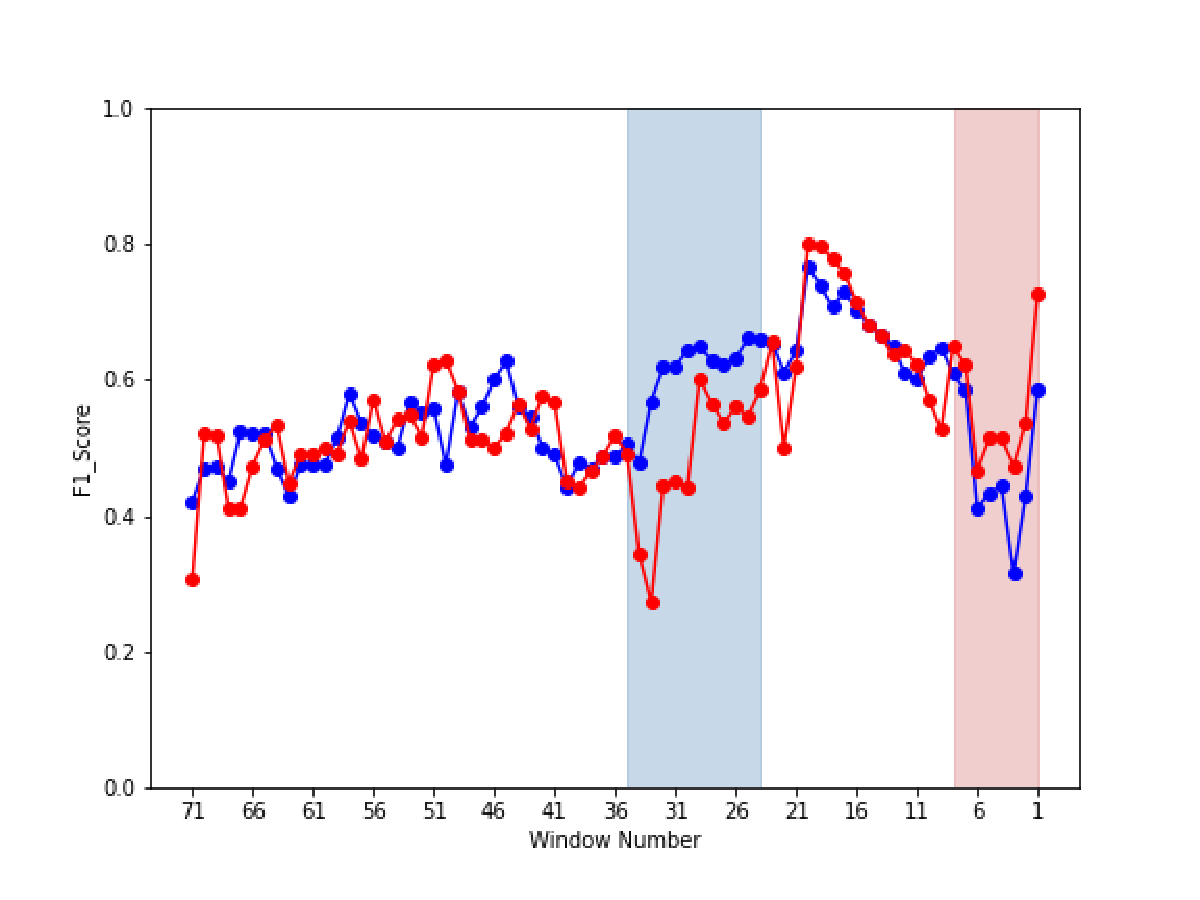
\includegraphics[width=0.495\textwidth]{Uenaka_fig/RQ2_result/Swift/Swift_review_F1.pdf}
    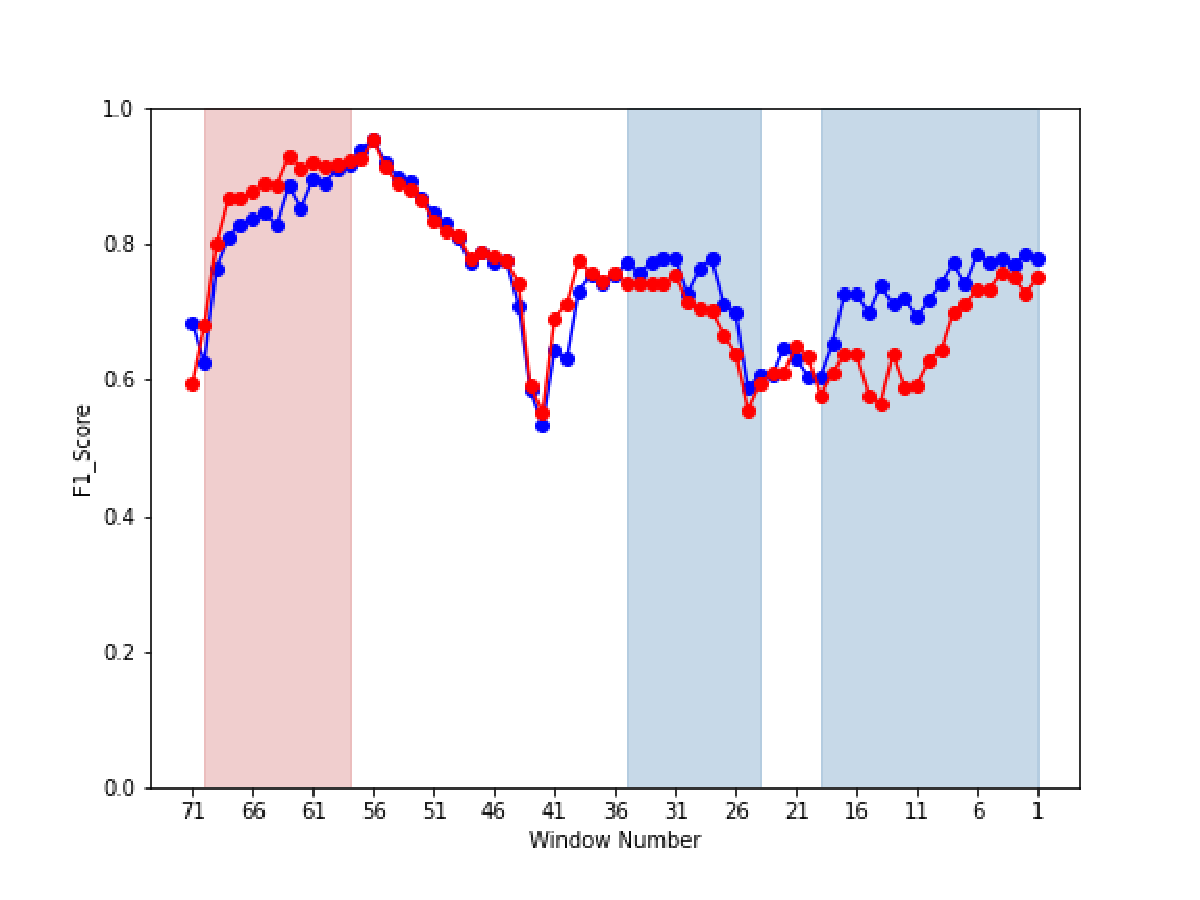
\includegraphics[width=0.495\textwidth]{Uenaka_fig/RQ2_result/Glance/Glance_review_F1.pdf}
    \caption{レビュー予測モデルのF値(上段左:Nova,上段右:Neutron,中段左:Cinder,\\ 中段右:Keystone,下段左:Swift,下段右:Glance)(赤:提案モデル,青:ベースラインモデル)}
    \label{fig:review_f}
\end{center}
\end{figure}
%-----------------------


\subsection{マージ予測モデル}
マージ予測モデルの予測結果として,図\ref{fig:merge_p}は適合率,図\ref{fig:merge_r}は再現率,図\ref{fig:merge_spec}は特異度,図\ref{fig:merge_f}はF値を示す.図は横軸,縦軸や折れ線,図の配置や色で表されている期間の定義は\ref{sec:rq2_review}項と同様である.また,図\ref{fig:merge_prepare_P}から図\ref{fig:merge_prepare_F}の定義に関しても\ref{sec:rq2_review}項と同様である.

図\ref{fig:merge_prepare_P}から図\ref{fig:merge_prepare_F}の結果から,開発状況に関する説明変数を用いることで,リリースまでの全期間における予測性能の差の平均はKeystoneプロジェクトを除き,適合率:-0.05〜+0.05,再現率:-0.05〜+0.02,特異度:-0.01〜+0.04,F値:-0.08〜+0.02程度の変化にとどまるという結果が得られた.この結果から,リリースまでの全期間においては,提案モデルの予測性能にはわずかな向上しか見られなかった.しかし,再現率以外の評価指標においては,全てのプロジェクトで向上期間が存在するため,ベースラインモデルよりも高い性能を示す期間を確認したが,性能が高くなる時期はプロジェクトによって異なる.そのため,プロジェクトごとに図\ref{fig:merge_prepare_P}から図\ref{fig:merge_prepare_F}における各評価指標の中でも特に特異度およびF値に着目し,向上期間の結果を解釈することで,各プロジェクトにおいて開発状況の説明変数が予測において有効に機能する時期を明らかにする.

\textbf{ (Nova) }特異度は前期において向上し,F値は中期および後期において向上するという結果が得られた.また,図\ref{fig:merge_prepare_R}から,F値の向上期間において再現率が向上したため,開発状況に関する説明変数を用いることで,正例と負例で異なる期間において網羅率が向上した.
また,図\ref{fig:merge_prepare_S},図\ref{fig:merge_prepare_F}における特異度およびF値の差の平均値から,開発状況に関する説明変数を用いることで,リリースまでの期間の中でも特に中期および後期ではレビュアによってマージすると判断されるチケットの予測性能が向上し,前期ではマージしないと判断されるチケットの予測性能が向上するという結果が得られた.
% 開発状況の説明変数はリリースまでの期間の中でも中期および後期ではマージされるチケットの予測において有効に機能し,前期ではマージされないチケットの予測において有効に機能するという結果が得られた.
% 提案モデルはリリースまでの期間の中でも中期および後期においてマージされるチケットの予測に有用であり,前期においてマージされないチケットの予測に有用であると考えられる.

\textbf{ (Neutron) }前期および中期において特異度が向上し,前期の一部期間においてF値が向上するという結果が得られた.また,図\ref{fig:merge_p},図\ref{fig:merge_r}から,F値の向上期間において適合率および再現率が向上したため,開発状況に関する説明変数を用いることで,前期において予測性能が向上した.
また,図\ref{fig:merge_prepare_S},図\ref{fig:merge_prepare_F}における特異度およびF値の差の平均値から,開発状況に関する説明変数を用いることで,リリースまでの期間の中でも特に前期ではレビュアによってマージする/しないと判断されるチケットの予測性能が向上するという結果が得られた.
% 開発状況の説明変数はリリースまでの期間の中でも前期において有効に機能するという結果が得られた.
% 提案モデルはリリースまでの期間の中でも前期において有用であると考えられる.

\textbf{ (Cinder) }前期および中期の一部期間において特異度が向上し,後期においてF値が向上するという結果が得られた.また,図\ref{fig:merge_prepare_R}から,F値の向上期間において再現率が向上したため,開発状況に関する説明変数を用いることで,正例と負例で異なる期間において網羅率が向上した.
また,図\ref{fig:merge_prepare_S},図\ref{fig:merge_prepare_F}における特異度およびF値の差の平均値から,開発状況に関する説明変数を用いることで,リリースまでの期間の中でも特に後期ではレビュアによってマージすると判断されるチケットの予測性能が向上し,前期ではマージしないと判断されるチケットの予測性能が向上するという結果が得られた.
% 開発状況の説明変数はリリースまでの期間の中でも後期ではマージされるチケットの予測において有効に機能し,前期ではマージされないチケットの予測において有効に機能するという結果が得られた.
% 提案モデルはリリースまでの期間の中でも後期においてマージされるチケットの予測に有用であり,前期においてマージされないチケットの予測に有用であると考えられる.

\textbf{ (Keystone) }前期および中期において特異度が向上し,中期の一部期間においてF値が向上するという結果が得られた.図\ref{fig:merge_prepare_P},図\ref{fig:merge_prepare_R}から,F値の向上期間において適合率および再現率が向上したため,開発状況に関する説明変数を用いることで,正例と負例で異なる期間において予測性能が向上した.
また,図\ref{fig:merge_prepare_S},図\ref{fig:merge_prepare_F}における特異度およびF値の差の平均値から,開発状況に関する説明変数を用いることで,リリースまでの期間の中でも特に中期ではレビュアによってマージすると判断されるチケットの予測性能が向上し,前期ではマージしないと判断されるチケットの予測性能が向上するという結果が得られた.
% 開発状況の説明変数はリリースまでの期間の中でも中期ではマージされるチケットの予測において有効に機能し,前期ではマージされないチケットの予測において有効に機能するという結果が得られた.
% 提案モデルはリリースまでの期間の中でも中期においてマージされるチケットの予測に有用であり,前期においてマージされないチケットの予測に有用であると考えられる.

\textbf{ (Swift) }前期および中期において特異度が向上し,後期においてF値が向上するという結果が得られた.また,図\ref{fig:merge_prepare_R}から,F値の向上期間において再現率が向上したため,開発状況に関する説明変数を用いることで,正例と負例で異なる期間において網羅率が向上した.
また,図\ref{fig:merge_prepare_S},図\ref{fig:merge_prepare_F}における特異度およびF値の差の平均値から,開発状況に関する説明変数を用いることで,リリースまでの期間の中でも特に後期ではレビュアによってマージすると判断されるチケットの予測性能が向上し,前期および中期ではマージしないと判断されるチケットの予測性能が向上するという結果が得られた.
% 開発状況の説明変数はリリースまでの期間の中でも後期ではマージされるチケットの予測において有効に機能し,前期および中期ではマージされないチケットの予測において有効に機能するという結果が得られた.
% 提案モデルはリリースまでの期間の中でも後期においてマージされるチケットの予測に有用であり,前期および中期においてマージされないチケットの予測に有用であると考えられる.

\textbf{ (Glance) }前期および中期において特異度が向上し,中期および後期の一部期間においてF値が向上するという結果が得られた.また,図\ref{fig:merge_prepare_P}から,F値の向上期間において適合率が向上したため,開発状況に関する説明変数を用いることで,中期および後期の一部期間において予測の正確性が向上した.
また,図\ref{fig:merge_prepare_S},図\ref{fig:merge_prepare_F}における特異度およびF値の差の平均値から,開発状況に関する説明変数を用いることで,リリースまでの期間の中でも特に中期ではレビュアによってマージすると判断されるチケットの予測性能が向上し,前期ではマージしないと判断されるチケットの予測性能が向上するという結果が得られた.
% 開発状況の説明変数はリリースまでの期間の中でも中期ではマージされるチケットの予測において有効に機能し,前期ではマージされないチケットの予測において有効に機能するという結果が得られた.
% 提案モデルはリリースまでの期間の中でも中期においてマージされるチケットの予測に有用であり,前期においてマージされないチケットの予測に有用であると考えられる.

これらの結果を踏まえ,\ref{sec:rq2_kousatu}節でマージされるチケットの予測において重要となった開発状況に関する説明変数を明らかにする.

\vskip\baselineskip
\fbox{\parbox{0.95\linewidth}{\textbf{(結果のまとめ)}マージされるチケットの予測において,Keystoneプロジェクトを除き,開発状況に関する説明変数を用いることで,リリースまでの期間全体では予測性能は平均で-0.08〜+0.05程度の変化にとどまった.また,プロジェクトごとに異なったリリースまでの期間において,特異度は平均で0.02〜0.10,F値は平均で0.07〜0.14程度,ベースラインモデルと比べて予測性能が向上する.}}

%-----------------------
\begin{figure}[t]
\begin{center}
    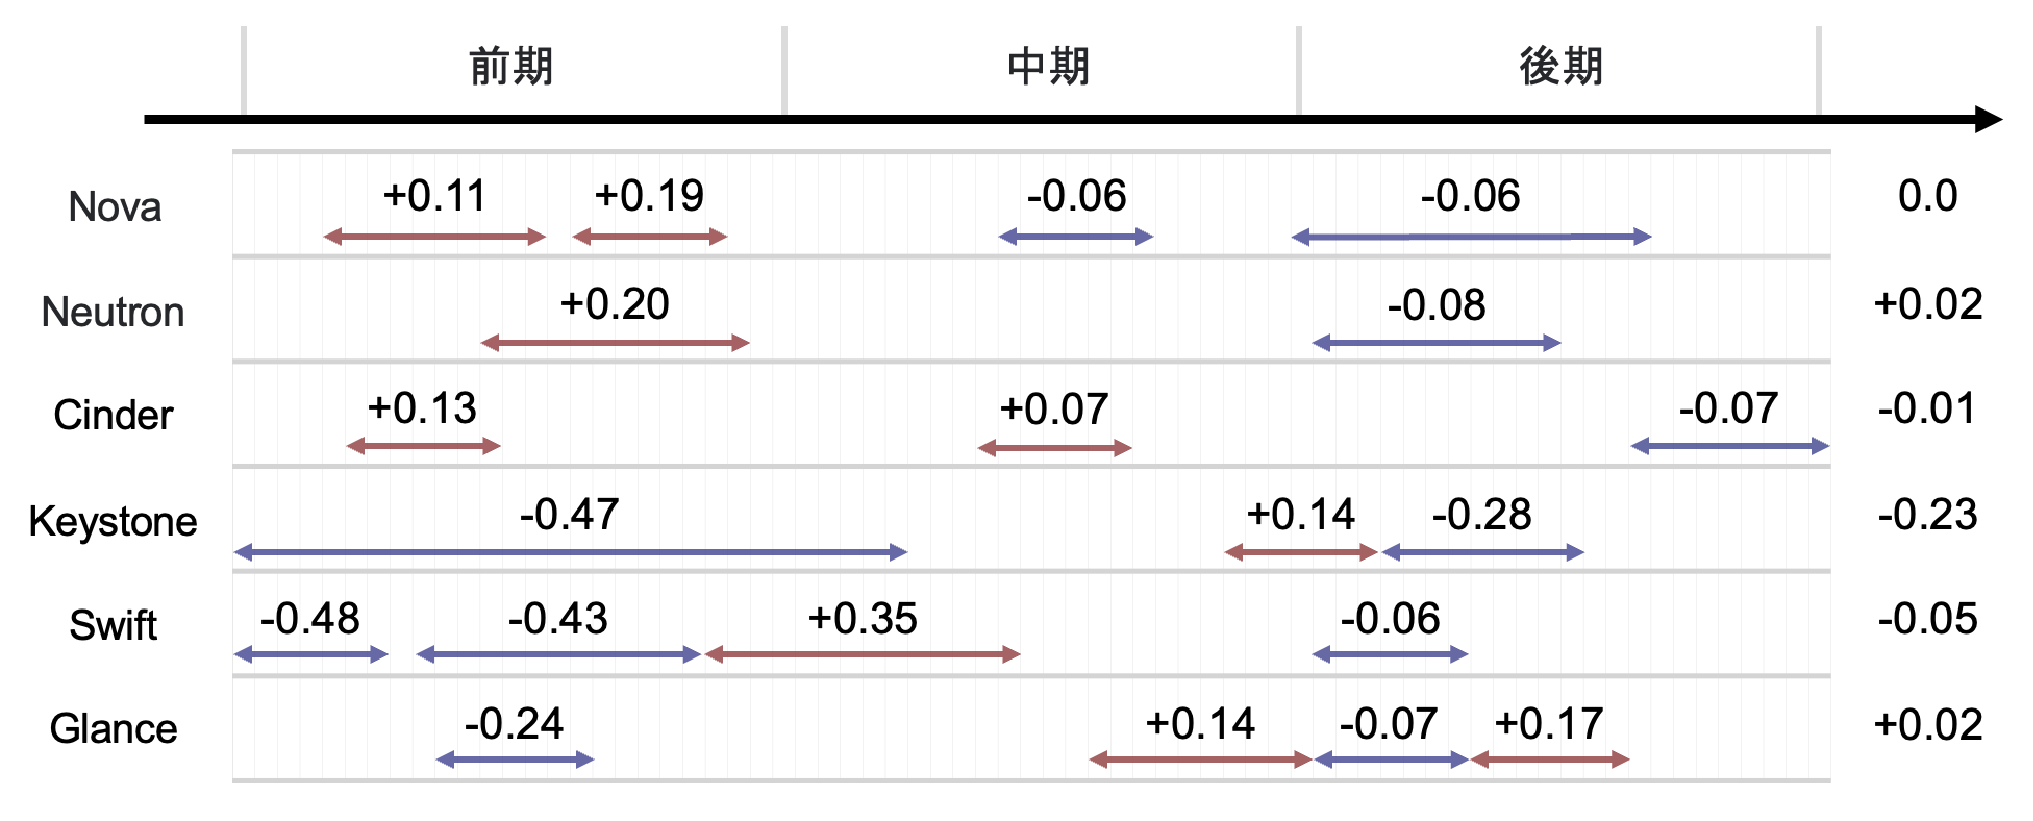
\includegraphics[width=1.0\textwidth]{Uenaka_fig/RQ2_result/merge_P.pdf}
    \caption{向上期間,低下期間,リリースまでの全期間における適合率の差の平均値}
    \label{fig:merge_prepare_P}
\end{center}
\end{figure}
%-----------------------

%-----------------------
\begin{figure}[t]
\begin{center}
    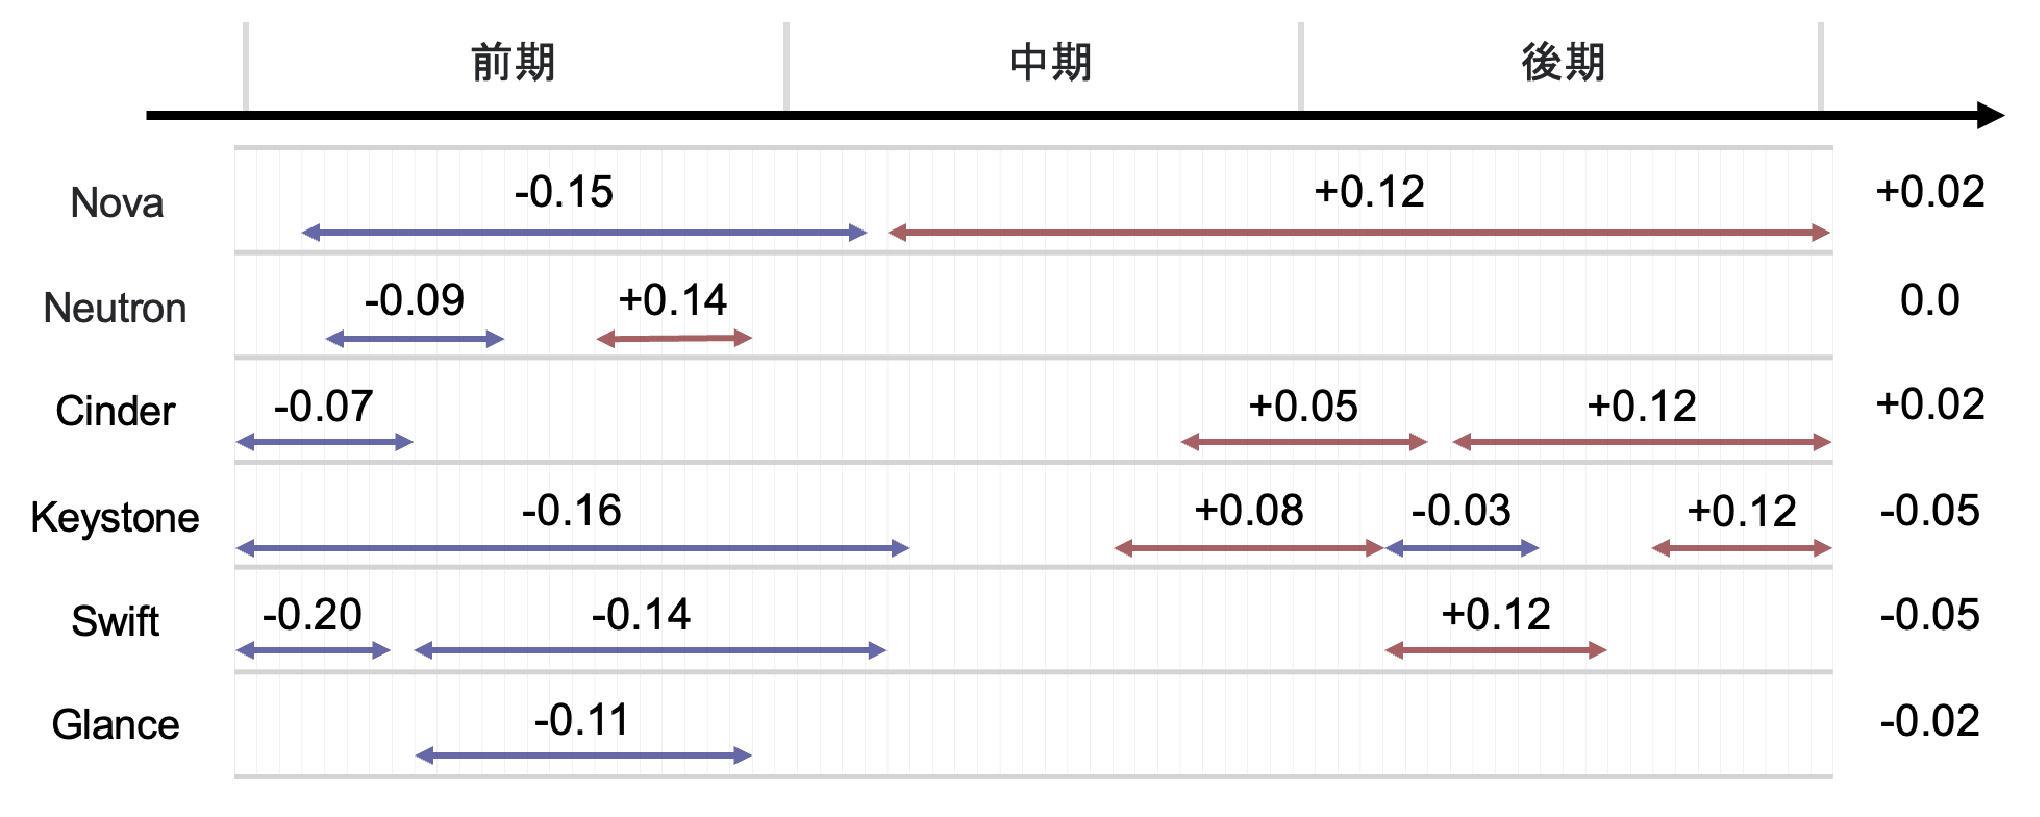
\includegraphics[width=1.0\textwidth]{Uenaka_fig/RQ2_result/merge_R.pdf}
    \caption{向上期間,低下期間,リリースまでの全期間における再現率の差の平均値}
    \label{fig:merge_prepare_R}
\end{center}
\end{figure}
%-----------------------

%-----------------------
\begin{figure}[t]
\begin{center}
    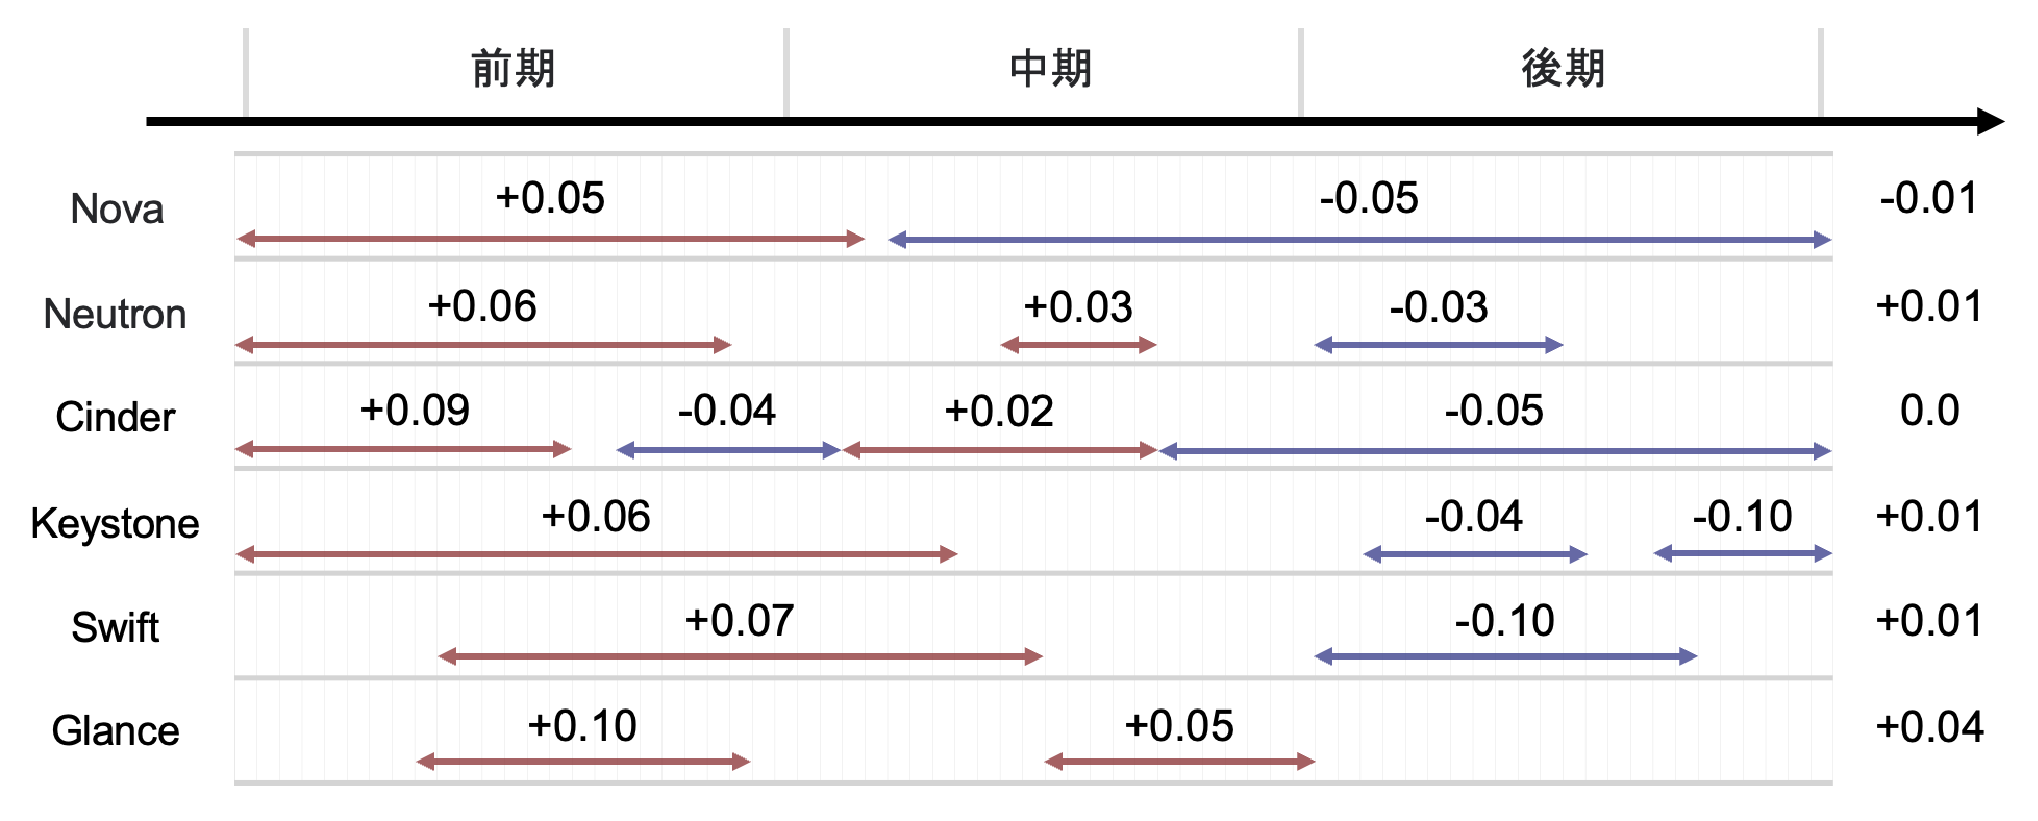
\includegraphics[width=1.0\textwidth]{Uenaka_fig/RQ2_result/merge_S.pdf}
    \caption{向上期間,低下期間,リリースまでの全期間における特異度の差の平均値}
    \label{fig:merge_prepare_S}
\end{center}
\end{figure}
%-----------------------

%-----------------------
\begin{figure}[t]
\begin{center}
    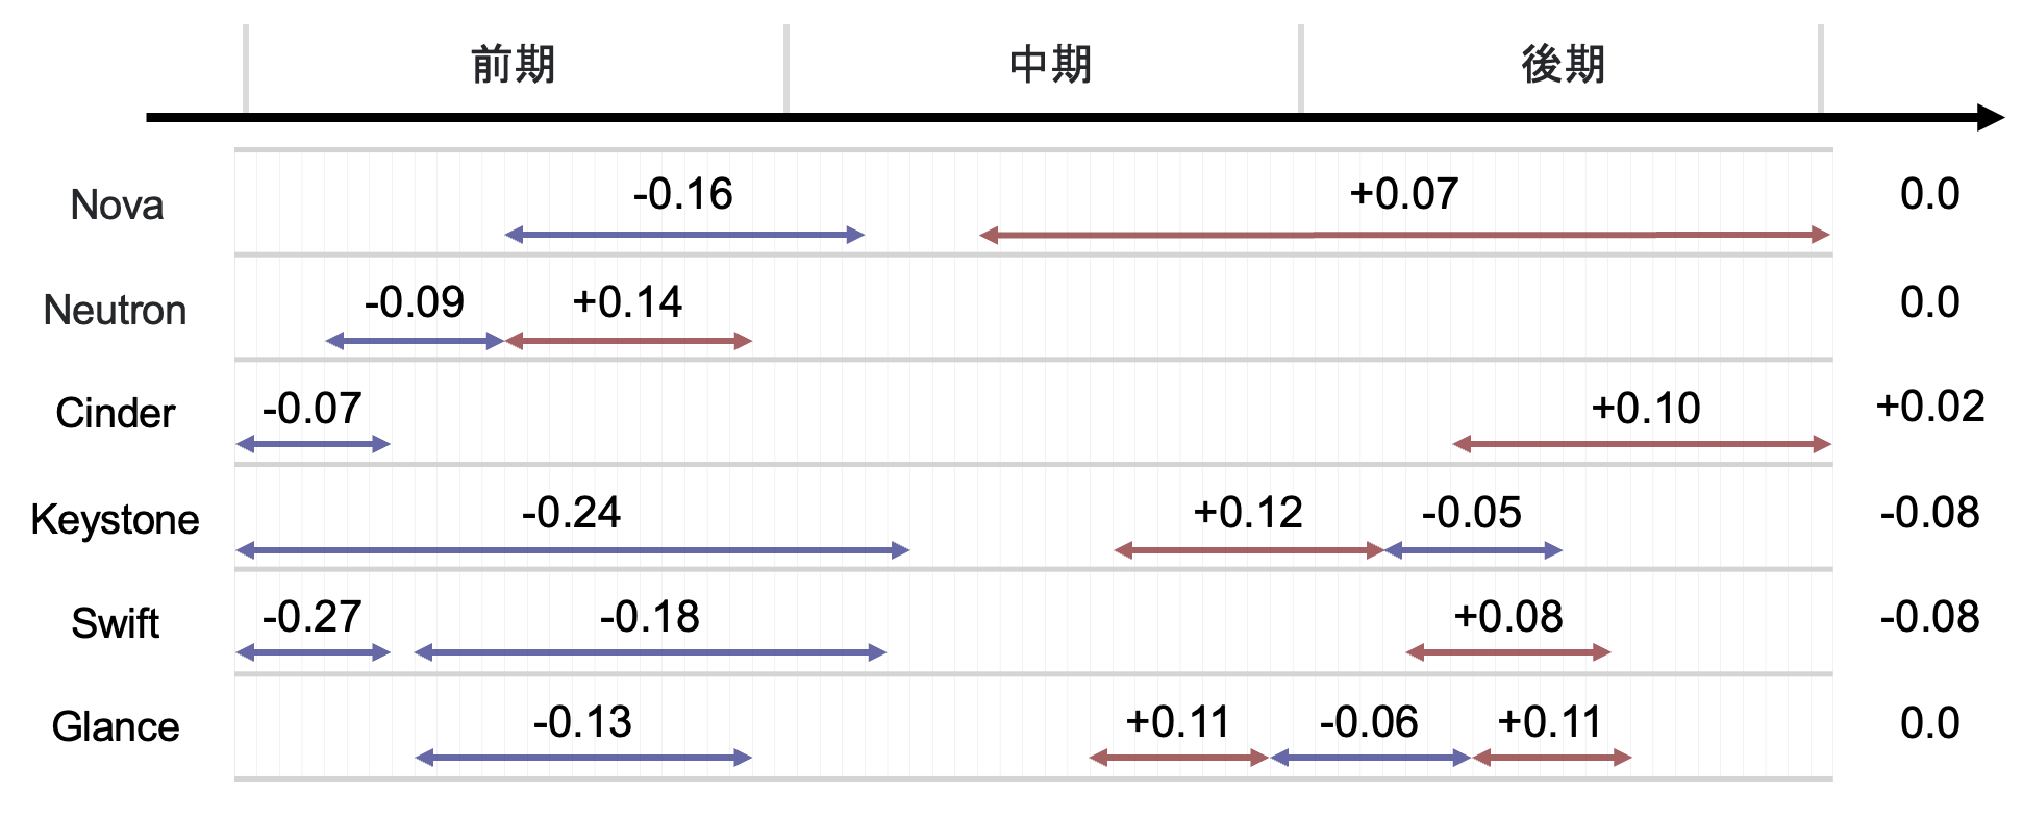
\includegraphics[width=1.0\textwidth]{Uenaka_fig/RQ2_result/merge_F.pdf}
    \caption{向上期間,低下期間,リリースまでの全期間におけるF値の差の平均値}
    \label{fig:merge_prepare_F}
\end{center}
\end{figure}
%-----------------------



%-----------------------
\clearpage
\begin{figure}[t]
\begin{minipage}{\textwidth}
\vspace{0.08\textheight}
\begin{center}
    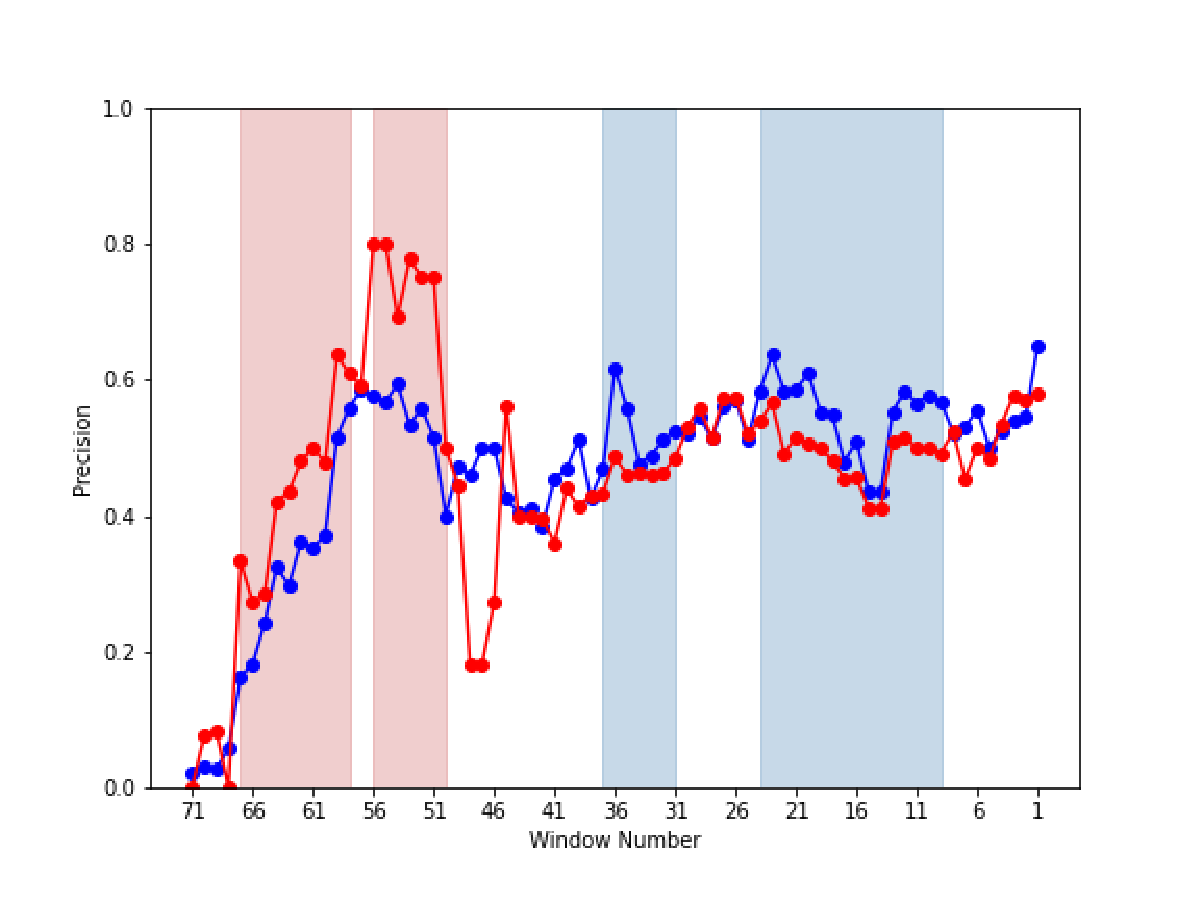
\includegraphics[width=0.495\textwidth]{Uenaka_fig/RQ2_result/Nova/Nova_merge_Precision.pdf}
    \includegraphics[width=0.495\textwidth]{Uenaka_fig/RQ2_result/Neutron/Neutron_merge_Precision.pdf}
    \includegraphics[width=0.495\textwidth]{Uenaka_fig/RQ2_result/Cinder/Cinder_merge_Precision.pdf}
    \includegraphics[width=0.495\textwidth]{Uenaka_fig/RQ2_result/Keystone/Keystone_merge_Precision.pdf}
    \includegraphics[width=0.495\textwidth]{Uenaka_fig/RQ2_result/Swift/Swift_merge_Precision.pdf}
    \includegraphics[width=0.495\textwidth]{Uenaka_fig/RQ2_result/Glance/Glance_merge_Precision.pdf}
    \caption{マージ予測モデルの適合率(上段左:Nova,上段右:Neutron,中段左:Cinder,\\ 中段右:Keystone,下段左:Swift,下段右:Glance)(赤:提案モデル,青:ベースラインモデル)}
    \label{fig:merge_p}
\end{center}
\vspace{0.08\textheight}
\end{minipage}
\end{figure}
%-----------------------

%-----------------------
\begin{figure}[t]
\begin{minipage}{\textwidth}
\vspace{0.08\textheight}
\begin{center}
    \includegraphics[width=0.495\textwidth]{Uenaka_fig/RQ2_result/Nova/Nova_merge_Recall.pdf}
    \includegraphics[width=0.495\textwidth]{Uenaka_fig/RQ2_result/Neutron/Neutron_merge_Recall.pdf}
    \includegraphics[width=0.495\textwidth]{Uenaka_fig/RQ2_result/Cinder/Cinder_merge_Recall.pdf}
    \includegraphics[width=0.495\textwidth]{Uenaka_fig/RQ2_result/Keystone/Keystone_merge_Recall.pdf}
    \includegraphics[width=0.495\textwidth]{Uenaka_fig/RQ2_result/Swift/Swift_merge_Recall.pdf}
    \includegraphics[width=0.495\textwidth]{Uenaka_fig/RQ2_result/Glance/Glance_merge_Recall.pdf}
    \caption{マージ予測モデルの再現率(上段左:Nova,上段右:Neutron,中段左:Cinder,\\ 中段右:Keystone,下段左:Swift,下段右:Glance)(赤:提案モデル,青:ベースラインモデル)}
    \label{fig:merge_r}
\end{center}
\vspace{0.08\textheight}
\end{minipage}
\end{figure}
%-----------------------

%-----------------------
\begin{figure}[t]
\begin{minipage}{\textwidth}
\vspace{0.08\textheight}
\begin{center}
    \includegraphics[width=0.495\textwidth]{Uenaka_fig/RQ2_result/Nova/Nova_merge_Specificity.pdf}
    \includegraphics[width=0.495\textwidth]{Uenaka_fig/RQ2_result/Neutron/Neutron_merge_Specificity.pdf}
    \includegraphics[width=0.495\textwidth]{Uenaka_fig/RQ2_result/Cinder/Cinder_merge_Specificity.pdf}
    \includegraphics[width=0.495\textwidth]{Uenaka_fig/RQ2_result/Keystone/Keystone_merge_Specificity.pdf}
    \includegraphics[width=0.495\textwidth]{Uenaka_fig/RQ2_result/Swift/Swift_merge_Specificity.pdf}
    \includegraphics[width=0.495\textwidth]{Uenaka_fig/RQ2_result/Glance/Glance_merge_Specificity.pdf}
    \caption{マージ予測モデルの特異度(上段左:Nova,上段右:Neutron,中段左:Cinder,\\ 中段右:Keystone,下段左:Swift,下段右:Glance)(赤:提案モデル,青:ベースラインモデル)}
    \label{fig:merge_spec}
\end{center}
\vspace{0.08\textheight}
\end{minipage}
\end{figure}
%-----------------------

%-----------------------
\begin{figure}[t]
\begin{center}
    \includegraphics[width=0.495\textwidth]{Uenaka_fig/RQ2_result/Nova/Nova_merge_F1.pdf}
    \includegraphics[width=0.495\textwidth]{Uenaka_fig/RQ2_result/Neutron/Neutron_merge_F1.pdf}
    \includegraphics[width=0.495\textwidth]{Uenaka_fig/RQ2_result/Cinder/Cinder_merge_F1.pdf}
    \includegraphics[width=0.495\textwidth]{Uenaka_fig/RQ2_result/Keystone/Keystone_merge_F1.pdf}
    \includegraphics[width=0.495\textwidth]{Uenaka_fig/RQ2_result/Swift/Swift_merge_F1.pdf}
    \includegraphics[width=0.495\textwidth]{Uenaka_fig/RQ2_result/Glance/Glance_merge_F1.pdf}
    \caption{マージ予測モデルのF値(上段左:Nova,上段右:Neutron,中段左:Cinder,\\ 中段右:Keystone,下段左:Swift,下段右:Glance)(赤:提案モデル,青:ベースラインモデル)}
    \label{fig:merge_f}
\end{center}
\end{figure}
%-----------------------


\section{考察:予測において重要となった開発状況に関する説明変数}\label{sec:rq2_kousatu}
RQ2ではレビューが開始される/マージされるチケットの予測において,開発状況を学習することで,リリースまでの一部の期間で予測性能が向上することを明らかにした.本節では,リリースまでの期間内で提案モデルのみで正しく判別したチケットの特徴量を分析することで,予測において重要となった開発状況に関する説明変数を明らかにする.具体的には,\ref{sec:rq1_kousatu2}節で用いたTree SHAPを用いて各ウィンドウでのテスト時の説明変数の重要度を算出する.また,\ref{sec:rq2_result}節の図\ref{fig:review_prepare_S},図\ref{fig:review_prepare_F},図\ref{fig:merge_prepare_S},図\ref{fig:merge_prepare_F}におけるF値および特異度の結果を元に,各プロジェクトにおいてF値および特異度が最も向上した期間のウィンドウ(最も向上した期間が複数存在した場合はより長い期間のウィンドウ)を抽出する.そして,各ウィンドウにおいて提案モデルのみで正しく判別したチケットの説明変数の重要度から,提案モデルのみで正しく判別したチケットの予測において重要となった開発状況に関する説明変数を明らかにする.

\subsection{レビュー予測モデル}\label{sec:rq2_kousatu_review}
表\ref{table:review_importance_propose_only_p}は,各プロジェクトで抽出したウィンドウにおいて,レビューが開始されるチケットの予測で重要度の高い説明変数と重要度を示す.また,表\ref{table:review_importance_propose_only_n}は,レビューが開始されないチケットの予測で重要度の高い説明変数と重要度を示す.表\ref{table:review_importance_propose_only_p}および表\ref{table:review_importance_propose_only_n}において,開発状況に関する説明変数は太字で表す.
また,図\ref{fig:review_review_num}および図\ref{fig:review_ticket_num}は,それぞれ提案モデルでレビュアのレビュー行数が重要度の高いプロジェクトにおけるレビュアのレビュー行数,提案モデルで予測対象チケット数が重要度の高いプロジェクトにおける予測対象チケット数を示す.図\ref{fig:review_review_num}および図\ref{fig:review_ticket_num}では,表\ref{table:review_importance_propose_only_p}および表\ref{table:review_importance_propose_only_n}におけるウィンドウの期間を赤色で表している.

表\ref{table:review_importance_propose_only_p}および表\ref{table:review_importance_propose_only_n}から,レビュー予測モデルでは,Novaプロジェクト以外の全てのプロジェクトにおいて開発状況に関する説明変数は重要度が高いという結果が得られた.具体的には,表\ref{table:review_importance_propose_only_p}から,レビューが開始されるチケットの予測においては,リリースまでの残り日数は1プロジェクト (Keystone) ,予測対象チケット数は3プロジェクト (Cinder, Swift, Glance) ,レビュアのレビュー行数は2プロジェクト (Neutron, Glance) で重要度が高いという結果が得られた.また,表\ref{table:review_importance_propose_only_n}から,レビューが開始されないチケットの予測においては,リリースまでの残り日数は1プロジェクト (Keystone) ,予測対象チケット数は1プロジェクト (Neutron) ,レビュアのレビュー行数は2プロジェクト (Swift, Glance) で重要度が高いという結果が得られた.

表\ref{table:review_importance_propose_only_p},表\ref{table:review_importance_propose_only_n}および図\ref{fig:review_review_num},図\ref{fig:review_ticket_num}の結果から,開発状況に関する各説明変数の結果を考察する.

\textbf{(リリースまでの残り日数)}表\ref{table:review_importance_propose_only_p}および表\ref{table:review_importance_propose_only_n}から,リリースまでの残り日数の重要度が高いウィンドウにおいて,リリースまでの残り日数は少ないという結果が得られた.この結果から,Keystoneプロジェクトでは,リリースまでの残り日数が少ない時期において,バージョン間で共通の優先基準が存在することが示唆される.

\textbf{(レビュアのレビュー行数)}図\ref{fig:review_review_num}から,レビュアのレビュー行数の重要度が高いウィンドウにおいて,レビュアのレビュー行数はNeutron,Glanceプロジェクトでは一貫した傾向がない一方,Swiftプロジェクトでは中程度であるという結果が得られた.この結果から,Swiftプロジェクトでは,レビュアのレビュー行数が中程度の時期において,バージョン間で共通の優先基準が存在することが示唆される.

\textbf{(予測対象チケット数)}図\ref{fig:review_ticket_num}から,予測対象チケット数の重要度が高いウィンドウにおいて,予測対象チケット数はNeutron,Glanceプロジェクトでは多い一方,Cinder,Swiftプロジェクトでは少ないという結果が得られた.この結果から,Neutron,Glanceプロジェクトでは,予測対象チケット数が多い時期においてバージョン間で共通の優先基準が存在することが示唆され,Cinder,Swiftプロジェクトでは予測対象チケット数が少ない時期においてバージョン間で共通の優先基準が存在することが示唆される.

これらの結果から,多数のプロジェクトにおいて,特定の開発状況下では,異なるバージョン間でレビューが開始されるチケットについて共通の優先基準が存在することが示唆される.


\begin{table}[t]
\caption{提案モデルのみで正例と正しく判別したチケットの予測で重要度の高い説明変数と重要度}
\label{table:review_importance_propose_only_p}
\centering
\vspace{0.5zh}
\scalebox{0.68}{
\begin{tabular}{l|c|cc|cc|cc}
    \hline \hline
    \multirow{2}{*}{プロジェクト}   & \multicolumn{1}{l|}{\multirow{2}{*}{ウィンドウ}} & \multicolumn{2}{c|}{1位} & \multicolumn{2}{c|}{2位} & \multicolumn{2}{c}{3位}  \\ \cline{3-8}
    & \multicolumn{1}{c|}{}  & 説明変数名 & \multicolumn{1}{c|}{重要度} & 説明変数名 & \multicolumn{1}{c|}{重要度} & 説明変数名 & \multicolumn{1}{c}{重要度} \\ \hline
    Nova  & 59〜71 & 経過時間  & 0.09 & ファイル数  & 0.00  & リビジョン数 & 0.00  \\
    Neutron  & 62〜71 & \textbf{レビュアのレビュー行数}  & 0.02  & 経過時間  & 0.02 & 削除行数 & 0.02  \\
    Cinder   & 24〜56 & \textbf{予測対象チケット数}  & 0.04  & マージ実績  & 0.03  & 報告実績 & 0.02  \\
    Keystone & 8〜17 & 直近報告実績  & 0.05  & バグ修正確信度  & 0.04  & \textbf{リリースまでの残り日数} & 0.03  \\
    Swift    & 1〜8 & 経過時間  & 0.05  & \textbf{予測対象チケット数}  & 0.02  & 削除行数 & 0.01  \\
    Glance   & 58〜70 & マージ実績  & 0.03  & \textbf{レビュアのレビュー行数}  & 0.02  & \textbf{予測対象チケット数}  & 0.02  \\ \hline
\end{tabular}}
\end{table}

\begin{table}[t]
\caption{提案モデルのみで負例と正しく判別したチケットの予測で重要度の高い説明変数と重要度}
\label{table:review_importance_propose_only_n}
\centering
\vspace{0.5zh}
\scalebox{0.72}{
\begin{tabular}{l|c|cc|cc|cc}
    \hline \hline
    \multirow{2}{*}{プロジェクト}   & \multicolumn{1}{l|}{\multirow{2}{*}{ウィンドウ}} & \multicolumn{2}{c|}{1位} & \multicolumn{2}{c|}{2位} & \multicolumn{2}{c}{3位}  \\ \cline{3-8}
    & \multicolumn{1}{c|}{}  & 説明変数名 & \multicolumn{1}{c|}{重要度} & 説明変数名 & \multicolumn{1}{c|}{重要度} & 説明変数名 & \multicolumn{1}{c}{重要度} \\ \hline
    Nova  & 1〜17 & 報告実績  & -0.01 & 直近報告実績  & -0.01  & 削除行数 & -0.01  \\
    Neutron  & 18〜33 & \textbf{予測対象チケット数}  & -0.02  & 報告実績  & -0.01 & 削除行数 & -0.01  \\
    Cinder   & 43〜67 & 報告実績  & -0.03  & 追加行数 & -0.02  & 直近報告実績  & -0.02  \\
    Keystone & 8〜15 & 報告実績  & -0.04  & \textbf{リリースまでの残り日数} & -0.03  & バグ修正確信度  & -0.03  \\
    Swift    & 25〜35 & \textbf{レビュアのレビュー行数}  & -0.04  & 経過時間  & -0.04  & 追加行数 & -0.02  \\
    Glance   & 58〜65 & \textbf{レビュアのレビュー行数}  & -0.02  & \textbf{予測対象チケット数}  & -0.02  & リビジョン数  & -0.02  \\ \hline
\end{tabular}}
\end{table}



%-----------------------
\begin{figure}[t]
\begin{center}
    \includegraphics[width=0.495\textwidth]{Uenaka_fig/RQ2_kousatu/Neutron_review_num.pdf}
    \includegraphics[width=0.495\textwidth]{Uenaka_fig/RQ2_kousatu/Swift_review_num.pdf}
    \includegraphics[width=0.495\textwidth]{Uenaka_fig/RQ2_kousatu/Glance_review_num.pdf}
    \caption{提案モデルでレビュアのレビュー行数が重要度の高いプロジェクトにおけるレビュアのレビュー行数(上段左:Neutron,上段右:Swift,下段:Glance)}
    \label{fig:review_review_num}
\end{center}
\end{figure}
%-----------------------

%-----------------------
\begin{figure}[t]
\begin{center}
    \includegraphics[width=0.495\textwidth]{Uenaka_fig/RQ2_kousatu/Neutron_ticket_num.pdf}
    \includegraphics[width=0.495\textwidth]{Uenaka_fig/RQ2_kousatu/Cinder_ticket_num.pdf}
    \includegraphics[width=0.495\textwidth]{Uenaka_fig/RQ2_kousatu/Swift_ticket_num.pdf}
    \includegraphics[width=0.495\textwidth]{Uenaka_fig/RQ2_kousatu/Glance_ticket_num.pdf}
    \caption{提案モデルで予測対象チケット数が重要度の高いプロジェクトにおける予測対象チケット数(上段左:Neutron,上段右:Cinder,下段左:Swift,下段右:Glance)}
    \label{fig:review_ticket_num}
\end{center}
\end{figure}
%-----------------------



\subsection{マージ予測モデル}
表\ref{table:merge_importance_propose_only_p}は,各プロジェクトで抽出したウィンドウにおいて,マージされるチケットの予測で重要度の高い説明変数と重要度を示す.また,表\ref{table:merge_importance_propose_only_n}は,マージされないチケットの予測で重要度の高い説明変数と重要度を示す.表\ref{table:merge_importance_propose_only_p}および表\ref{table:merge_importance_propose_only_n}においても,\ref{sec:rq2_kousatu_review}節と同様に,開発状況に関する説明変数は太字で表す.
また,図\ref{fig:merge_ticket_num}は,提案モデルで予測対象チケット数が重要度の高いプロジェクトにおける予測対象チケット数を示す.図\ref{fig:merge_ticket_num}において,表\ref{table:merge_importance_propose_only_n}における色で表されている期間の定義は\ref{sec:rq2_kousatu_review}節と同様である.
表\ref{table:merge_importance_propose_only_p}および表\ref{table:merge_importance_propose_only_n}から,マージ予測モデルでは,\ref{sec:rq1_kousatu2}節と同様に経過時間が最も重要度が高い説明変数であるという結果が得られた.一方で,マージされるチケットの予測においては,リリースまでの残り日数が4プロジェクト (Nova, Cinder, Keystone, Swift) で重要度が高いという結果が得られた.また,マージされないチケットの予測においては,予測対象チケット数が2プロジェクト (Nova, Swift) で重要度が高いという結果が得られた.

表\ref{table:merge_importance_propose_only_p},表\ref{table:merge_importance_propose_only_n}および図\ref{fig:merge_ticket_num}の結果から,開発状況に関する各説明変数の結果を考察する.

\textbf{(リリースまでの残り日数)}表\ref{table:merge_importance_propose_only_p}から,リリースまでの残り日数の重要度が高いウィンドウにおいて,リリースまでの残り日数は少ないという結果が得られた.この結果から,4プロジェクト (Nova, Cinder, Keystone, Swift) では,リリースまでの残り日数が少ない時期において,バージョン間で共通の優先基準が存在することが示唆される.

\textbf{(予測対象チケット数)}図\ref{fig:merge_ticket_num}から,予測対象チケット数の重要度が高いウィンドウにおいて,予測対象チケット数はNovaプロジェクトでは一貫した傾向がない一方,Glanceプロジェクトでは少ないという結果が得られた.この結果から,Glanceプロジェクトでは,予測対象チケット数が少ない時期において,バージョン間で共通の優先基準が存在することが示唆される.

これらの結果から,多数のプロジェクトにおいて,特定の開発状況下では,異なるバージョン間でマージされるチケットについて共通の優先基準が存在することが示唆される.


\begin{table}[t]
\caption{提案モデルのみで正例と正しく判別したチケットの予測で重要度の高い説明変数と重要度}
\label{table:merge_importance_propose_only_p}
\centering
\vspace{0.5zh}
\scalebox{0.78}{
\begin{tabular}{l|c|cc|cc|cc}
    \hline \hline
    \multirow{2}{*}{プロジェクト}   & \multicolumn{1}{l|}{\multirow{2}{*}{ウィンドウ}} & \multicolumn{2}{c|}{1位} & \multicolumn{2}{c|}{2位} & \multicolumn{2}{c}{3位}  \\ \cline{3-8}
    & \multicolumn{1}{c|}{}  & 説明変数名 & \multicolumn{1}{c|}{重要度} & 説明変数名 & \multicolumn{1}{c|}{重要度} & 説明変数名 & \multicolumn{1}{c}{重要度} \\ \hline
    Nova  & 1〜38 & 経過時間  & 0.10 & \textbf{リリースまでの残り日数} & 0.04  & 直近マージ実績  & 0.02  \\
    Neutron  & 49〜59 & 経過時間  & 0.06  & 追加行数 & 0.05 & ファイル数 & 0.02  \\
    Cinder   & 1〜17 & 経過時間  & 0.07  & \textbf{リリースまでの残り日数} & 0.06  & 報告実績  & 0.01  \\
    Keystone & 21〜32 & 経過時間  & 0.10  & \textbf{リリースまでの残り日数} & 0.10  & 直近マージ実績  & 0.02  \\
    Swift    & 11〜19 & 経過時間  & 0.09  & \textbf{リリースまでの残り日数} & 0.03  & ファイル数 & 0.01  \\
    Glance   & 26〜32 & 経過時間  & 0.13  & バグ修正確信度  & 0.03  & 直近マージ実績  & 0.02  \\ \hline
\end{tabular}}
\end{table}

\begin{table}[t]
\caption{提案モデルのみで負例と正しく判別したチケットの予測で重要度の高い説明変数と重要度}
\label{table:merge_importance_propose_only_n}
\centering
\vspace{0.5zh}
\scalebox{0.8}{
\begin{tabular}{l|c|cc|cc|cc}
    \hline \hline
    \multirow{2}{*}{プロジェクト}   & \multicolumn{1}{l|}{\multirow{2}{*}{ウィンドウ}} & \multicolumn{2}{c|}{1位} & \multicolumn{2}{c|}{2位} & \multicolumn{2}{c}{3位}  \\ \cline{3-8}
    & \multicolumn{1}{c|}{}  & 説明変数名 & \multicolumn{1}{c|}{重要度} & 説明変数名 & \multicolumn{1}{c|}{重要度} & 説明変数名 & \multicolumn{1}{c}{重要度} \\ \hline
    Nova  & 44〜71 & 経過時間  & -0.04 & \textbf{予測対象チケット数}  & -0.04  & 直近マージ実績  & 0.00  \\
    Neutron  & 50〜71 & 経過時間  & -0.05  & 追加行数  & -0.04 & マージ実績  & -0.01  \\
    Cinder   & 57〜71 & 経過時間  & -0.04  & 追加行数  & -0.01  & 直近報告実績 & -0.01  \\
    Keystone & 40〜71 & 経過時間  & -0.03  & テストコード含有  & -0.01  & 直近報告実績 & -0.01  \\
    Swift    & 36〜62 & 経過時間  & -0.03  & \textbf{予測対象チケット数}  & -0.02  & バグ修正確信度  & -0.01  \\
    Glance   & 49〜63 & 経過時間  & -0.06  & バグ修正確信度  & -0.03  & 追加行数  & -0.03  \\ \hline
\end{tabular}}
\end{table}


%-----------------------
\begin{figure}[t]
\begin{center}
    \includegraphics[width=0.495\textwidth]{Uenaka_fig/RQ2_kousatu/Nova_ticket_num.pdf}
    \includegraphics[width=0.495\textwidth]{Uenaka_fig/RQ2_kousatu/Swift_ticket_num_merge.pdf}
    \caption{提案モデルで予測対象チケット数が重要度の高いプロジェクトにおける予測対象チケット数(左:Nova,右:Swift)}
    \label{fig:merge_ticket_num}
\end{center}
\end{figure}
%-----------------------


%%%%%%%%%%%%%%%%%%%%%%
\section{妥当性の脅威}\label{sec:disc}
%%%%%%%%%%%%%%%%%%%%%%

\section{内的妥当性}
本研究で取り扱うレビュー予測モデルでは,ウィンドウ内の2週間より前にレビューが開始されたチケットは既に優先されたチケットとみなし分析対象外としている.しかし,開発者がレビュアからの修正要求に基づき改修したソースコードを再報告した場合,レビュアはレビューが開始されていないチケットだけでなく再報告されたチケットも含めて,優先してレビューするチケットを選択していることが示唆される.ただし,本研究では,レビューが開始されていないチケットの中で,優先的にレビューされるチケットがリリースまでの期間によってどのように変化するのかに焦点を当てている.そのため,再報告されたチケットが分析結果のノイズとなることを防ぐことで,レビューが開始されていないチケットについての十分な知見を得ることができたと考える.

本研究では,従来研究\cite{prioritizer}で提案されているチケットおよび開発者の特徴(7種類)と従来研究\cite{release_merge}\cite{review1}の知見から有用と示唆される開発者や変更内容の特徴(5種類)を説明変数に用いてベースラインモデルを構築したため,チケットのソースコード変更に関する特徴量(例えば,複雑度)など,より詳細なソースコードレベルの特徴量を説明変数に用いることで予測性能が向上することが示唆される.ただし,本研究でデータセットとして用いたOpenStackプロジェクトのコアコンポーネント6プロジェクトが利用するGerritでは,コードレビューチケットのリストを閲覧できる機能が提供されている.本研究では主に上記のリストから取得可能な情報をもとに特徴量を収集することで,脅威を削減する.

\section{外的妥当性}
本研究では,ケーススタディとしてOpenStackプロジェクトのコアコンポーネント6プロジェクトのコードレビューチケットを対象とした.対象とするプロジェクトやリリースバージョンを変更した場合に分析結果および予測精度が変化することが示唆される.しかし,本研究ではGerritを利用するプロジェクトの中でもコードレビューチケットが多く提案されているOpenStackプロジェクトのコアコンポーネントプロジェクトを対象としている.また,その中でもマージされたチケットの多いバージョンを対象とすることで,脅威を削減する.


%%%%%%%%%%%%%%%%%%%%%%
\section{おわりに}\label{sec:fig-tab-exp}
%%%%%%%%%%%%%%%%%%%%%%
本論文では,時期ごとにバージョン間で共通の優先基準が存在し,その基準に応じてチケットが優先される場合と優先されなくなる場合があると考え,リリースまでの期間に焦点を当てた研究を行った.従来手法と同様にチケットおよび開発者の特徴を説明変数とする予測モデルと,追加で開発状況を説明変数として用いる予測モデルの2種類のモデルを構築し,1日ごとに学習またはテストを行うことで,両モデルの予測性能を算出した.リリースまでの期間における予測性能の変化を分析することで,2つのリサーチクエスチョン (RQ) を検証した.

RQ1では,チケットおよび開発者の特徴を説明変数とする予測モデルの予測性能がリリースまでの期間内でどの程度変化するかを分析した.4種類の評価指標を用いてモデルの予測性能を評価した結果,チケットおよび開発者の特徴を説明変数とする予測モデルの予測性能の変動幅は,レビューが開始されるチケットの予測において0.16〜0.53,マージされるチケットの予測において0.11〜0.95であり,リリースまでの期間内で大きく変化することを明らかにした.また,全てのプロジェクトにおいて,チケットおよび開発者の特徴の中でもチケットが報告されてからの経過時間が最も重要度が高く,負例のチケットと比べ,正例のチケットの経過時間が短いことを明らかにした.この結果から,全てのプロジェクトにおいて,レビュアは経過時間の短いチケットの優先順位を高く見積もる傾向にあることが示唆される.

また,RQ2では,開発状況に関する説明変数を用いることで,予測性能はリリースまでの期間によってどの程度変化するかを分析した.結果として,提案モデルのF値はベースラインモデルと比べて,プロジェクトごとに異なったリリースまでの期間において,レビューが開始されるチケットの予測で0.02〜0.09程度,マージされるチケットの予測で0.07〜0.14向上した.また,提案モデルで予測性能が向上した期間において,提案モデルのみで正しく判別できたチケットの特徴量重要度を分析した結果,多数のプロジェクトにおいて開発状況に関する説明変数は予測における重要度が高いことを明らかにした.この結果から,多数のプロジェクトにおいて,特定の開発状況下では,異なるバージョン間で共通の優先基準が存在することが示唆される.

今後の研究として,プロジェクトごとにモデルを適応させるアプローチが重要な検討課題となる.本論文では,全てのプロジェクトに対して同一のモデルを用いて優先されるチケットを予測した.しかし,本論文で得られた知見から,チケットの優先基準はプロジェクトごとに異なると考えられる.そのため,今後は各プロジェクトに適したチューニングを施すことで,予測性能の向上が期待される.今後の研究において,この点を探究することが求められる.

本論文で明らかにしたリリースまでの期間などの開発状況による予測性能への影響より,優先度が日々変動するチケットの優先順位の決定に将来的に寄与できると考える.




\bibliographystyle{ipsjunsrt}
\bibliography{bibfile_IPSJjournal_Uenaka}

\vspace{-4mm}

\begin{biography}
\profile{m}{伊原 彰紀}{2009年奈良先端科学技術大学院大学情報科学研究科博士前期課程修了.2012年同大学博士後期課程修了.2012年同大学情報科学研究科助教.2018年和歌山大学システム工学部講師.博士(工学).ソフトウェア工学,特にオープンソースソフトウェア開発・利用支援の研究に従事.電子情報通信学会,IEEE各会員.}
%
\profile{n}{上中 瑞稀}{2024年和歌山大学システム工学部在学中,ソフトウェア工学,特にプログラム検証の研究に従事.}
\end{biography}



\end{document}
